% Capitolul 4: Sezonalitate și prognoză: SARIMA, TBATS, Prophet
% Serii de timp -- Programele de licență Informatică economică și Cibernetică economică, Academia de Studii Economice din București
% GENERAT de latex/build_chapter4.py -- modificați generatorul, nu acest fișier.

\newcommand{\coursename}{Serii de timp}
\def\tsalang{ro}
% Preambul comun TSA -- Serii de timp / Time Series Analysis (Beamer, 16:9)
% Același design ca MFM și SFM (preluat din SFM, 5 octombrie 2026). Înainte de % Preambul comun TSA -- Serii de timp / Time Series Analysis (Beamer, 16:9)
% Același design ca MFM și SFM (preluat din SFM, 5 octombrie 2026). Înainte de % Preambul comun TSA -- Serii de timp / Time Series Analysis (Beamer, 16:9)
% Același design ca MFM și SFM (preluat din SFM, 5 octombrie 2026). Înainte de \input{../../latex/preamble} se definește
%   \newcommand{\coursename}{Time Series Analysis}      (EN)
%   \newcommand{\coursename}{Serii de timp}       (RO)  și  \def\tsalang{ro}
% Fișierele .tex se află în EN/Courses, EN/Seminars, RO/Cursuri, RO/Seminarii (două niveluri sub rădăcină).
% Deck-urile sînt generate de latex/build_chapterN.py / build_seminarN.py (vezi latex/tsa_build.py).

\documentclass[9pt, aspectratio=169, t]{beamer}
\providecommand{\coursename}{Time Series Analysis}

% Ensure content fits on slides
\setbeamersize{text margin left=8mm, text margin right=8mm}
% Smaller institute font (title page)
\setbeamerfont{institute}{size=\footnotesize}

%=============================================================================
% THEME AND STYLE CONFIGURATION
%=============================================================================
\usetheme{default}
% Using default theme for clean header/footer control

% Color Palette (matching Redispatch PDF)
\definecolor{MainBlue}{RGB}{26, 58, 110}
\definecolor{AccentBlue}{RGB}{26, 58, 110}
\definecolor{IDAred}{RGB}{205, 0, 0}
\definecolor{DarkGray}{RGB}{51, 51, 51}
\definecolor{MediumGray}{RGB}{128, 128, 128}
\definecolor{LightGray}{RGB}{248, 248, 248}
\definecolor{VeryLightGray}{RGB}{235, 235, 235}
\definecolor{KeynoteGray}{RGB}{218, 218, 218}
\definecolor{SectionGray}{RGB}{120, 120, 120}
\definecolor{FooterGray}{RGB}{100, 100, 100}
\definecolor{Crimson}{RGB}{220, 53, 69}
\definecolor{Forest}{RGB}{46, 125, 50}
\definecolor{Amber}{RGB}{181, 133, 63}
\definecolor{Orange}{RGB}{230, 126, 34}
\definecolor{Purple}{RGB}{142, 68, 173}

% Gradient background (exact Keynote 315° gradient: white to RGB 218,218,218)
\setbeamertemplate{background}{%
    \begin{tikzpicture}[remember picture, overlay]
        \shade[shading=axis, shading angle=315,
        top color=white, bottom color=KeynoteGray]
        (current page.south west) rectangle (current page.north east);
    \end{tikzpicture}%
}
% Fallback solid color for compatibility
\setbeamercolor{background canvas}{bg=}

\setbeamercolor{palette primary}{bg=MainBlue, fg=white}
\setbeamercolor{palette secondary}{bg=MainBlue!85, fg=white}
\setbeamercolor{palette tertiary}{bg=MainBlue!70, fg=white}
\setbeamercolor{structure}{fg=MainBlue}
\setbeamercolor{title}{fg=IDAred}
\setbeamercolor{frametitle}{fg=IDAred, bg=}
\setbeamercolor{block title}{bg=MainBlue, fg=white}
\setbeamercolor{block body}{bg=VeryLightGray, fg=DarkGray}
\setbeamercolor{block title alerted}{bg=Crimson, fg=white}
\setbeamercolor{block body alerted}{bg=Crimson!8, fg=DarkGray}
\setbeamercolor{block title example}{bg=Forest, fg=white}
\setbeamercolor{block body example}{bg=Forest!8, fg=DarkGray}
\setbeamercolor{item}{fg=MainBlue}

% Footer colors (override Madrid theme blue)
\setbeamercolor{author in head/foot}{fg=FooterGray, bg=}
\setbeamercolor{title in head/foot}{fg=FooterGray, bg=}
\setbeamercolor{date in head/foot}{fg=FooterGray, bg=}
\setbeamercolor{section in head/foot}{fg=FooterGray, bg=}
\setbeamercolor{subsection in head/foot}{fg=FooterGray, bg=}

% Bullet styles (apply everywhere including blocks)
\setbeamertemplate{itemize item}{\color{MainBlue}$\boxdot$}
\setbeamertemplate{itemize subitem}{\color{MainBlue}$\blacktriangleright$}
\setbeamertemplate{itemize subsubitem}{\color{MainBlue}\tiny$\bullet$}
\setbeamertemplate{itemize/enumerate body begin}{\normalsize}
\setbeamertemplate{itemize/enumerate subbody begin}{\normalsize}

% Item spacing - compact style
\setlength{\leftmargini}{10pt}       % Level 1: minimal indent
\setlength{\leftmarginii}{10pt}      % Level 2: minimal additional indent
% Compact list spacing (zero extra space before/after lists in blocks)
\makeatletter
\def\@listi{\leftmargin\leftmargini \topsep 0pt \parsep 0pt \itemsep 0pt}
\def\@listii{\leftmargin\leftmarginii \topsep 0pt \parsep 0pt \itemsep 0pt}
\makeatother

\setbeamertemplate{navigation symbols}{}

%=============================================================================
% CUSTOM HEADLINE
%=============================================================================
\setbeamertemplate{headline}{%
    \vskip10pt%
    \hbox to \paperwidth{%
        \hskip0.5cm%
        {\small\color{FooterGray}\renewcommand{\hyperlink}[2]{##2}\insertsectionhead}%
        \hfill%
        \textcolor{FooterGray}{\small\insertframenumber}%
        \hskip0.5cm%
    }%
    \vskip4pt%
    {\color{FooterGray}\hrule height 0.4pt}%
}

%=============================================================================
% CUSTOM FOOTER
%=============================================================================
\usepackage{fontawesome5}

\setbeamertemplate{footline}{%
    {\color{FooterGray}\hrule height 0.4pt}%
    \vskip4pt%
    \hbox to \paperwidth{%
        \hskip0.5cm%
        \textcolor{FooterGray}{\small\coursename}%
        \hfill%
        \raisebox{-0.1em}{%
            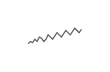
\begin{tikzpicture}[x=0.08em, y=0.08em, line width=0.4pt]
                \draw[FooterGray] (0,3) -- (1,4) -- (2,3.5) -- (3,5) -- (4,4) -- (5,6) -- (6,5.5) -- (7,4) -- (8,5) -- (9,7) -- (10,6) -- (11,5) -- (12,6.5) -- (13,8) -- (14,7) -- (15,6) -- (16,7.5) -- (17,9) -- (18,8) -- (19,7) -- (20,8.5) -- (21,10) -- (22,9) -- (23,8) -- (24,9.5);
            \end{tikzpicture}%
        }%
        \hskip0.5cm%
    }%
    \vskip6pt%
}

%=============================================================================
% PACKAGES
%=============================================================================
\usepackage[utf8]{inputenc}
\DeclareUnicodeCharacter{03B1}{\ensuremath{\alpha}}
\usepackage[T1]{fontenc}
\usepackage{amsmath, amssymb, amsthm}
\usepackage{mathtools}
\usepackage{bm}
\usepackage{tikz}
\usetikzlibrary{arrows.meta, positioning, shapes, calc, decorations.pathreplacing, shadings}
\usepackage{booktabs}
\usepackage{multirow}
\usepackage{array}
\usepackage{graphicx}
\usepackage{animate}
\usepackage{hyperref}
\usepackage{colortbl}
\usepackage{listings}
\lstset{language=Python, basicstyle=\ttfamily\scriptsize, keywordstyle=\color{MainBlue}\bfseries,
  commentstyle=\color{Forest}, stringstyle=\color{Crimson}, breaklines=true,
  frame=none, backgroundcolor=\color{VeryLightGray}, xleftmargin=2mm}
\hypersetup{colorlinks=true, linkcolor=MainBlue, urlcolor=MainBlue}
\graphicspath{{../../logos/}{../../charts/}{../../photos/}}
\usepackage{xcolor}
\hfuzz=2pt  % Suppress tiny overfull warnings (<2pt)
\vfuzz=2pt  % Suppress tiny vertical overfull warnings (<2pt)
% \mathrm in the sans-serif family of the slides (beamer resets \mathrm to the serif family at \begin{document};
% this hook runs after beamer's, so WN, Var, RMSE, ... in formulas match the surrounding text)
% Bold vectors and matrices in the same sans-serif family: \mathbf{A} in sans bold (beamer's own \mathbf came out in
% medium weight), and the bold upright Greek capitals of \boldsymbol / \bm (\bSigma, \bPhi, \boldsymbol{\Theta}) in
% cmss bold: bm.sty fixes its "boldoperators" font when it is loaded (serif cmbx), before beamer switches the
% operators to cmss, so it is reset here.
\AtBeginDocument{%
  \SetMathAlphabet{\mathrm}{normal}{\encodingdefault}{\sfdefault}{\mddefault}{n}%
  \SetMathAlphabet{\mathrm}{bold}{\encodingdefault}{\sfdefault}{bx}{n}%
  \SetMathAlphabet{\mathbf}{normal}{\encodingdefault}{\sfdefault}{bx}{n}%
  \SetMathAlphabet{\mathbf}{bold}{\encodingdefault}{\sfdefault}{bx}{n}%
  \SetSymbolFont{boldoperators}{normal}{OT1}{cmss}{bx}{n}%
  \SetSymbolFont{boldoperators}{bold}{OT1}{cmss}{bx}{n}}

%=============================================================================
% QUANTLET COMMANDS
%   \quantlet{<displayed name>}{<url>}       (generic, compatible with the older TSA decks)
%   \tsaquantlet{Ch_05}{TSA_ch5_garch}       -> https://github.com/danpele/Time-Series-Analysis/tree/main/Quantlets/Ch_05/TSA_ch5_garch
%   \qlurl{<folder>} is defined per chapter by the generator (Quantlets/Ch_NN/<folder>)
%=============================================================================
\newcommand{\tsarepo}{https://github.com/danpele/Time-Series-Analysis}
\newcommand{\tsaqlbase}{https://github.com/danpele/Time-Series-Analysis/tree/main/Quantlets}
\newcommand{\quantlet}[2]{%
    \hfill\href{#2}{%
        \raisebox{-0.15em}{
\includegraphics[height=0.7em]{ql_logo.png}}%
        \textcolor{MainBlue}{\tiny\ #1}%
    }%
}
\newcommand{\tsaquantlet}[2]{\quantlet{\detokenize{#2}}{\tsaqlbase/#1/#2}}

%=============================================================================
% NOTEBOOKS (Google Colab)
%   \colaburl{notebooks/EN/chapter5_seminar_notebook.ipynb} -> the Colab link of a file in the TSA repo
%   \nb: the chapter notebook (each seminar deck redefines it with \renewcommand)
%=============================================================================
\newcommand{\colaburl}[1]{https://colab.research.google.com/github/danpele/Time-Series-Analysis/blob/main/#1}
\newcommand{\nb}{https://colab.research.google.com/github/danpele/Time-Series-Analysis/tree/main/notebooks/EN}
\newcommand{\nbname}{notebooks/EN}

%=============================================================================
% SLIDE HELPERS (used by the generators; the same as in MFM)
%=============================================================================
% local font size for list bodies (the preamble forces \normalsize)
\newcommand{\itemsize}[1]{\setbeamertemplate{itemize/enumerate body begin}{#1}\setbeamertemplate{itemize/enumerate subbody begin}{#1}}
\newcommand{\intitle}[1]{{\hypersetup{urlcolor=white}#1}}   % white links inside coloured title bars
\newcommand{\imgcap}[1]{{\scriptsize #1}\\[0.5mm]}          % caption under a photo
\newcommand{\imgcredit}[2]{{\tiny\color{FooterGray}\href{#1}{#2}}}   % image credit: source URL, author/licence
\newcommand{\aiprompt}[1]{{\ttfamily\color{MainBlue}#1}}     % a prompt to an AI assistant

%=============================================================================
% SEMINARS: student version by default; the instructor wrapper *_solutions.tex sets \solutionstrue
%=============================================================================
\makeatletter\@ifundefined{ifsolutions}{\expandafter\newif\csname ifsolutions\endcsname}{}\makeatother
\newcommand{\solonly}[1]{\ifsolutions #1\fi}
\newcommand{\propsub}{\ifsolutions\else\framesubtitle{\ifdefined\tsalang Rezolvarea se discută la seminar\else Solution discussed in class\fi}\fi}

%=============================================================================
% APPENDIX AND CHAPTER LINKS (latex/appendix_links.py writes the calls; it also re-declares these
% macros before \begin{document}, so the decks compile with or without this preamble block)
%=============================================================================
\providecommand{\tsaapplink}[3]{\hypertarget{#2}{}\hyperlink{#1}{\beamergotobutton{#3}}}
\providecommand{\tsaappback}[2]{\begin{tikzpicture}[remember picture,overlay]\node[anchor=south east] at ([xshift=-3mm,yshift=7mm]current page.south east){\hyperlink{#1}{\beamerreturnbutton{#2}}};\end{tikzpicture}}
\providecommand{\tsachlink}[2]{\href{#1}{#2}}
\providecommand{\tsachlinkt}[2]{\href{#1}{\usebeamercolor[fg]{frametitle}#2}}

%=============================================================================
% QUANTINAR COMMAND: link către un curs Quantinar (subiecte avansate)
%=============================================================================
\newcommand{\quantinar}[2]{%
    \href{#2}{%
        \raisebox{-0.15em}{
\includegraphics[height=0.8em]{qr_logo.png}}%
        \textcolor{MainBlue}{\scriptsize\ #1}%
    }%
}

%=============================================================================
% CUSTOM TITLE PAGE
%=============================================================================
\defbeamertemplate*{title page}{hybrid}[1][]
{
    \vspace{0.2cm}
    % Logos row - top header (with clickable links)
    \begin{center}
        \href{https://www.ase.ro}{
\includegraphics[height=1.0cm]{ase_logo.png}}\hspace{0.3cm}%
        \href{https://theida.net}{
\includegraphics[height=1.0cm]{ida_logo.png}}\hspace{0.3cm}%
        \href{https://blockchain-research-center.com}{
\includegraphics[height=1.0cm]{brc_logo.png}}\hspace{0.3cm}%
        \href{https://www.ai4efin.ase.ro}{
\includegraphics[height=1.0cm]{ai4efin_logo.png}}\hspace{0.3cm}%
        \href{https://ipe.ro/new}{
\includegraphics[height=1.0cm]{acad_logo.png}}\hspace{0.3cm}%
        \href{https://www.digital-finance-msca.com}{
\includegraphics[height=1.0cm]{msca_logo.png}}%
    \end{center}

    \vspace{0.6cm}

    % Main title with Q logos on sides (with clickable links)
    \begin{center}
        \begin{minipage}{0.1\textwidth}
            \centering
            \href{https://quantlet.com}{
\includegraphics[height=1.1cm]{ql_logo.png}}
        \end{minipage}%
        \begin{minipage}{0.78\textwidth}
            \centering
            {\LARGE\bfseries\usebeamercolor[fg]{title}\inserttitle}

            \vspace{0.3cm}

            {\usebeamerfont{subtitle}\usebeamercolor[fg]{title}\insertsubtitle}
        \end{minipage}%
        \begin{minipage}{0.1\textwidth}
            \centering
            \href{https://quantinar.com}{
\includegraphics[height=1.1cm]{qr_logo.png}}
        \end{minipage}
    \end{center}

    \vspace{0.6cm}

    % Authors (left aligned)
    \hspace{0.5cm}{\usebeamerfont{author}\insertauthor}

    \vspace{0.3cm}

    % Institute/Affiliations (left aligned)
    \hspace{0.5cm}\begin{minipage}[t]{0.9\textwidth}
        \raggedright\small\insertinstitute
    \end{minipage}
}

%=============================================================================
% THEOREM ENVIRONMENTS
%=============================================================================
\theoremstyle{definition}
\setbeamertemplate{theorems}[numbered]
\ifdefined\tsalang
\newtheorem{defn}{Definiție}
\newtheorem{thm}{Teoremă}
\newtheorem{prop}{Propoziție}
\newtheorem{rmk}{Observație}
\else
\newtheorem{defn}{Definition}
\newtheorem{thm}{Theorem}
\newtheorem{prop}{Proposition}
\newtheorem{rmk}{Remark}
\fi

%=============================================================================
% CENTRED MINIPAGE (no extra vertical space)
%=============================================================================
\newenvironment{cminipage}[1]{%
    \par\noindent\hfill\begin{minipage}{#1}\ignorespaces
}{%
    \end{minipage}\hfill\null\par
}

%=============================================================================
% CUSTOM COMMANDS
%=============================================================================
\newcommand{\E}{\mathbb{E}}
\newcommand{\Var}{\text{Var}}
\newcommand{\Cov}{\text{Cov}}
\newcommand{\Corr}{\text{Corr}}
\newcommand{\R}{\mathbb{R}}
\newcommand{\N}{\mathbb{N}}
\newcommand{\Z}{\mathbb{Z}}
\newcommand{\B}{\mathbf{B}}
\newcommand{\imark}{\textcolor{MainBlue}{\textbullet}}
\newcommand{\RMSE}{\text{RMSE}}
\newcommand{\MAE}{\text{MAE}}
\newcommand{\MAPE}{\text{MAPE}}

% Boldface vector/matrix commands (VAR, VECM, state space; also used by the older TSA decks)
\newcommand{\bY}{\mathbf{Y}}
\newcommand{\bX}{\mathbf{X}}
\newcommand{\bA}{\mathbf{A}}
\newcommand{\bB}{\mathbf{B}}
\newcommand{\bepsilon}{\boldsymbol{\varepsilon}}
\newcommand{\bSigma}{\boldsymbol{\Sigma}}
\newcommand{\bPhi}{\boldsymbol{\Phi}}
\newcommand{\bGamma}{\boldsymbol{\Gamma}}
\newcommand{\bPi}{\boldsymbol{\Pi}}
\newcommand{\bc}{\mathbf{c}}
\newcommand{\balpha}{\boldsymbol{\alpha}}
\newcommand{\bbeta}{\boldsymbol{\beta}}
\newcommand{\bvarepsilon}{\boldsymbol{\varepsilon}}

% Legacy seminar marks (older TSA seminar decks)
\newcommand{\correct}{\textcolor{Forest}{\checkmark}}
\newcommand{\incorrect}{\textcolor{Crimson}{\texttimes}}
 se definește
%   \newcommand{\coursename}{Time Series Analysis}      (EN)
%   \newcommand{\coursename}{Serii de timp}       (RO)  și  \def\tsalang{ro}
% Fișierele .tex se află în EN/Courses, EN/Seminars, RO/Cursuri, RO/Seminarii (două niveluri sub rădăcină).
% Deck-urile sînt generate de latex/build_chapterN.py / build_seminarN.py (vezi latex/tsa_build.py).

\documentclass[9pt, aspectratio=169, t]{beamer}
\providecommand{\coursename}{Time Series Analysis}

% Ensure content fits on slides
\setbeamersize{text margin left=8mm, text margin right=8mm}
% Smaller institute font (title page)
\setbeamerfont{institute}{size=\footnotesize}

%=============================================================================
% THEME AND STYLE CONFIGURATION
%=============================================================================
\usetheme{default}
% Using default theme for clean header/footer control

% Color Palette (matching Redispatch PDF)
\definecolor{MainBlue}{RGB}{26, 58, 110}
\definecolor{AccentBlue}{RGB}{26, 58, 110}
\definecolor{IDAred}{RGB}{205, 0, 0}
\definecolor{DarkGray}{RGB}{51, 51, 51}
\definecolor{MediumGray}{RGB}{128, 128, 128}
\definecolor{LightGray}{RGB}{248, 248, 248}
\definecolor{VeryLightGray}{RGB}{235, 235, 235}
\definecolor{KeynoteGray}{RGB}{218, 218, 218}
\definecolor{SectionGray}{RGB}{120, 120, 120}
\definecolor{FooterGray}{RGB}{100, 100, 100}
\definecolor{Crimson}{RGB}{220, 53, 69}
\definecolor{Forest}{RGB}{46, 125, 50}
\definecolor{Amber}{RGB}{181, 133, 63}
\definecolor{Orange}{RGB}{230, 126, 34}
\definecolor{Purple}{RGB}{142, 68, 173}

% Gradient background (exact Keynote 315° gradient: white to RGB 218,218,218)
\setbeamertemplate{background}{%
    \begin{tikzpicture}[remember picture, overlay]
        \shade[shading=axis, shading angle=315,
        top color=white, bottom color=KeynoteGray]
        (current page.south west) rectangle (current page.north east);
    \end{tikzpicture}%
}
% Fallback solid color for compatibility
\setbeamercolor{background canvas}{bg=}

\setbeamercolor{palette primary}{bg=MainBlue, fg=white}
\setbeamercolor{palette secondary}{bg=MainBlue!85, fg=white}
\setbeamercolor{palette tertiary}{bg=MainBlue!70, fg=white}
\setbeamercolor{structure}{fg=MainBlue}
\setbeamercolor{title}{fg=IDAred}
\setbeamercolor{frametitle}{fg=IDAred, bg=}
\setbeamercolor{block title}{bg=MainBlue, fg=white}
\setbeamercolor{block body}{bg=VeryLightGray, fg=DarkGray}
\setbeamercolor{block title alerted}{bg=Crimson, fg=white}
\setbeamercolor{block body alerted}{bg=Crimson!8, fg=DarkGray}
\setbeamercolor{block title example}{bg=Forest, fg=white}
\setbeamercolor{block body example}{bg=Forest!8, fg=DarkGray}
\setbeamercolor{item}{fg=MainBlue}

% Footer colors (override Madrid theme blue)
\setbeamercolor{author in head/foot}{fg=FooterGray, bg=}
\setbeamercolor{title in head/foot}{fg=FooterGray, bg=}
\setbeamercolor{date in head/foot}{fg=FooterGray, bg=}
\setbeamercolor{section in head/foot}{fg=FooterGray, bg=}
\setbeamercolor{subsection in head/foot}{fg=FooterGray, bg=}

% Bullet styles (apply everywhere including blocks)
\setbeamertemplate{itemize item}{\color{MainBlue}$\boxdot$}
\setbeamertemplate{itemize subitem}{\color{MainBlue}$\blacktriangleright$}
\setbeamertemplate{itemize subsubitem}{\color{MainBlue}\tiny$\bullet$}
\setbeamertemplate{itemize/enumerate body begin}{\normalsize}
\setbeamertemplate{itemize/enumerate subbody begin}{\normalsize}

% Item spacing - compact style
\setlength{\leftmargini}{10pt}       % Level 1: minimal indent
\setlength{\leftmarginii}{10pt}      % Level 2: minimal additional indent
% Compact list spacing (zero extra space before/after lists in blocks)
\makeatletter
\def\@listi{\leftmargin\leftmargini \topsep 0pt \parsep 0pt \itemsep 0pt}
\def\@listii{\leftmargin\leftmarginii \topsep 0pt \parsep 0pt \itemsep 0pt}
\makeatother

\setbeamertemplate{navigation symbols}{}

%=============================================================================
% CUSTOM HEADLINE
%=============================================================================
\setbeamertemplate{headline}{%
    \vskip10pt%
    \hbox to \paperwidth{%
        \hskip0.5cm%
        {\small\color{FooterGray}\renewcommand{\hyperlink}[2]{##2}\insertsectionhead}%
        \hfill%
        \textcolor{FooterGray}{\small\insertframenumber}%
        \hskip0.5cm%
    }%
    \vskip4pt%
    {\color{FooterGray}\hrule height 0.4pt}%
}

%=============================================================================
% CUSTOM FOOTER
%=============================================================================
\usepackage{fontawesome5}

\setbeamertemplate{footline}{%
    {\color{FooterGray}\hrule height 0.4pt}%
    \vskip4pt%
    \hbox to \paperwidth{%
        \hskip0.5cm%
        \textcolor{FooterGray}{\small\coursename}%
        \hfill%
        \raisebox{-0.1em}{%
            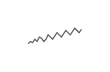
\begin{tikzpicture}[x=0.08em, y=0.08em, line width=0.4pt]
                \draw[FooterGray] (0,3) -- (1,4) -- (2,3.5) -- (3,5) -- (4,4) -- (5,6) -- (6,5.5) -- (7,4) -- (8,5) -- (9,7) -- (10,6) -- (11,5) -- (12,6.5) -- (13,8) -- (14,7) -- (15,6) -- (16,7.5) -- (17,9) -- (18,8) -- (19,7) -- (20,8.5) -- (21,10) -- (22,9) -- (23,8) -- (24,9.5);
            \end{tikzpicture}%
        }%
        \hskip0.5cm%
    }%
    \vskip6pt%
}

%=============================================================================
% PACKAGES
%=============================================================================
\usepackage[utf8]{inputenc}
\DeclareUnicodeCharacter{03B1}{\ensuremath{\alpha}}
\usepackage[T1]{fontenc}
\usepackage{amsmath, amssymb, amsthm}
\usepackage{mathtools}
\usepackage{bm}
\usepackage{tikz}
\usetikzlibrary{arrows.meta, positioning, shapes, calc, decorations.pathreplacing, shadings}
\usepackage{booktabs}
\usepackage{multirow}
\usepackage{array}
\usepackage{graphicx}
\usepackage{animate}
\usepackage{hyperref}
\usepackage{colortbl}
\usepackage{listings}
\lstset{language=Python, basicstyle=\ttfamily\scriptsize, keywordstyle=\color{MainBlue}\bfseries,
  commentstyle=\color{Forest}, stringstyle=\color{Crimson}, breaklines=true,
  frame=none, backgroundcolor=\color{VeryLightGray}, xleftmargin=2mm}
\hypersetup{colorlinks=true, linkcolor=MainBlue, urlcolor=MainBlue}
\graphicspath{{../../logos/}{../../charts/}{../../photos/}}
\usepackage{xcolor}
\hfuzz=2pt  % Suppress tiny overfull warnings (<2pt)
\vfuzz=2pt  % Suppress tiny vertical overfull warnings (<2pt)
% \mathrm in the sans-serif family of the slides (beamer resets \mathrm to the serif family at \begin{document};
% this hook runs after beamer's, so WN, Var, RMSE, ... in formulas match the surrounding text)
% Bold vectors and matrices in the same sans-serif family: \mathbf{A} in sans bold (beamer's own \mathbf came out in
% medium weight), and the bold upright Greek capitals of \boldsymbol / \bm (\bSigma, \bPhi, \boldsymbol{\Theta}) in
% cmss bold: bm.sty fixes its "boldoperators" font when it is loaded (serif cmbx), before beamer switches the
% operators to cmss, so it is reset here.
\AtBeginDocument{%
  \SetMathAlphabet{\mathrm}{normal}{\encodingdefault}{\sfdefault}{\mddefault}{n}%
  \SetMathAlphabet{\mathrm}{bold}{\encodingdefault}{\sfdefault}{bx}{n}%
  \SetMathAlphabet{\mathbf}{normal}{\encodingdefault}{\sfdefault}{bx}{n}%
  \SetMathAlphabet{\mathbf}{bold}{\encodingdefault}{\sfdefault}{bx}{n}%
  \SetSymbolFont{boldoperators}{normal}{OT1}{cmss}{bx}{n}%
  \SetSymbolFont{boldoperators}{bold}{OT1}{cmss}{bx}{n}}

%=============================================================================
% QUANTLET COMMANDS
%   \quantlet{<displayed name>}{<url>}       (generic, compatible with the older TSA decks)
%   \tsaquantlet{Ch_05}{TSA_ch5_garch}       -> https://github.com/danpele/Time-Series-Analysis/tree/main/Quantlets/Ch_05/TSA_ch5_garch
%   \qlurl{<folder>} is defined per chapter by the generator (Quantlets/Ch_NN/<folder>)
%=============================================================================
\newcommand{\tsarepo}{https://github.com/danpele/Time-Series-Analysis}
\newcommand{\tsaqlbase}{https://github.com/danpele/Time-Series-Analysis/tree/main/Quantlets}
\newcommand{\quantlet}[2]{%
    \hfill\href{#2}{%
        \raisebox{-0.15em}{
\includegraphics[height=0.7em]{ql_logo.png}}%
        \textcolor{MainBlue}{\tiny\ #1}%
    }%
}
\newcommand{\tsaquantlet}[2]{\quantlet{\detokenize{#2}}{\tsaqlbase/#1/#2}}

%=============================================================================
% NOTEBOOKS (Google Colab)
%   \colaburl{notebooks/EN/chapter5_seminar_notebook.ipynb} -> the Colab link of a file in the TSA repo
%   \nb: the chapter notebook (each seminar deck redefines it with \renewcommand)
%=============================================================================
\newcommand{\colaburl}[1]{https://colab.research.google.com/github/danpele/Time-Series-Analysis/blob/main/#1}
\newcommand{\nb}{https://colab.research.google.com/github/danpele/Time-Series-Analysis/tree/main/notebooks/EN}
\newcommand{\nbname}{notebooks/EN}

%=============================================================================
% SLIDE HELPERS (used by the generators; the same as in MFM)
%=============================================================================
% local font size for list bodies (the preamble forces \normalsize)
\newcommand{\itemsize}[1]{\setbeamertemplate{itemize/enumerate body begin}{#1}\setbeamertemplate{itemize/enumerate subbody begin}{#1}}
\newcommand{\intitle}[1]{{\hypersetup{urlcolor=white}#1}}   % white links inside coloured title bars
\newcommand{\imgcap}[1]{{\scriptsize #1}\\[0.5mm]}          % caption under a photo
\newcommand{\imgcredit}[2]{{\tiny\color{FooterGray}\href{#1}{#2}}}   % image credit: source URL, author/licence
\newcommand{\aiprompt}[1]{{\ttfamily\color{MainBlue}#1}}     % a prompt to an AI assistant

%=============================================================================
% SEMINARS: student version by default; the instructor wrapper *_solutions.tex sets \solutionstrue
%=============================================================================
\makeatletter\@ifundefined{ifsolutions}{\expandafter\newif\csname ifsolutions\endcsname}{}\makeatother
\newcommand{\solonly}[1]{\ifsolutions #1\fi}
\newcommand{\propsub}{\ifsolutions\else\framesubtitle{\ifdefined\tsalang Rezolvarea se discută la seminar\else Solution discussed in class\fi}\fi}

%=============================================================================
% APPENDIX AND CHAPTER LINKS (latex/appendix_links.py writes the calls; it also re-declares these
% macros before \begin{document}, so the decks compile with or without this preamble block)
%=============================================================================
\providecommand{\tsaapplink}[3]{\hypertarget{#2}{}\hyperlink{#1}{\beamergotobutton{#3}}}
\providecommand{\tsaappback}[2]{\begin{tikzpicture}[remember picture,overlay]\node[anchor=south east] at ([xshift=-3mm,yshift=7mm]current page.south east){\hyperlink{#1}{\beamerreturnbutton{#2}}};\end{tikzpicture}}
\providecommand{\tsachlink}[2]{\href{#1}{#2}}
\providecommand{\tsachlinkt}[2]{\href{#1}{\usebeamercolor[fg]{frametitle}#2}}

%=============================================================================
% QUANTINAR COMMAND: link către un curs Quantinar (subiecte avansate)
%=============================================================================
\newcommand{\quantinar}[2]{%
    \href{#2}{%
        \raisebox{-0.15em}{
\includegraphics[height=0.8em]{qr_logo.png}}%
        \textcolor{MainBlue}{\scriptsize\ #1}%
    }%
}

%=============================================================================
% CUSTOM TITLE PAGE
%=============================================================================
\defbeamertemplate*{title page}{hybrid}[1][]
{
    \vspace{0.2cm}
    % Logos row - top header (with clickable links)
    \begin{center}
        \href{https://www.ase.ro}{
\includegraphics[height=1.0cm]{ase_logo.png}}\hspace{0.3cm}%
        \href{https://theida.net}{
\includegraphics[height=1.0cm]{ida_logo.png}}\hspace{0.3cm}%
        \href{https://blockchain-research-center.com}{
\includegraphics[height=1.0cm]{brc_logo.png}}\hspace{0.3cm}%
        \href{https://www.ai4efin.ase.ro}{
\includegraphics[height=1.0cm]{ai4efin_logo.png}}\hspace{0.3cm}%
        \href{https://ipe.ro/new}{
\includegraphics[height=1.0cm]{acad_logo.png}}\hspace{0.3cm}%
        \href{https://www.digital-finance-msca.com}{
\includegraphics[height=1.0cm]{msca_logo.png}}%
    \end{center}

    \vspace{0.6cm}

    % Main title with Q logos on sides (with clickable links)
    \begin{center}
        \begin{minipage}{0.1\textwidth}
            \centering
            \href{https://quantlet.com}{
\includegraphics[height=1.1cm]{ql_logo.png}}
        \end{minipage}%
        \begin{minipage}{0.78\textwidth}
            \centering
            {\LARGE\bfseries\usebeamercolor[fg]{title}\inserttitle}

            \vspace{0.3cm}

            {\usebeamerfont{subtitle}\usebeamercolor[fg]{title}\insertsubtitle}
        \end{minipage}%
        \begin{minipage}{0.1\textwidth}
            \centering
            \href{https://quantinar.com}{
\includegraphics[height=1.1cm]{qr_logo.png}}
        \end{minipage}
    \end{center}

    \vspace{0.6cm}

    % Authors (left aligned)
    \hspace{0.5cm}{\usebeamerfont{author}\insertauthor}

    \vspace{0.3cm}

    % Institute/Affiliations (left aligned)
    \hspace{0.5cm}\begin{minipage}[t]{0.9\textwidth}
        \raggedright\small\insertinstitute
    \end{minipage}
}

%=============================================================================
% THEOREM ENVIRONMENTS
%=============================================================================
\theoremstyle{definition}
\setbeamertemplate{theorems}[numbered]
\ifdefined\tsalang
\newtheorem{defn}{Definiție}
\newtheorem{thm}{Teoremă}
\newtheorem{prop}{Propoziție}
\newtheorem{rmk}{Observație}
\else
\newtheorem{defn}{Definition}
\newtheorem{thm}{Theorem}
\newtheorem{prop}{Proposition}
\newtheorem{rmk}{Remark}
\fi

%=============================================================================
% CENTRED MINIPAGE (no extra vertical space)
%=============================================================================
\newenvironment{cminipage}[1]{%
    \par\noindent\hfill\begin{minipage}{#1}\ignorespaces
}{%
    \end{minipage}\hfill\null\par
}

%=============================================================================
% CUSTOM COMMANDS
%=============================================================================
\newcommand{\E}{\mathbb{E}}
\newcommand{\Var}{\text{Var}}
\newcommand{\Cov}{\text{Cov}}
\newcommand{\Corr}{\text{Corr}}
\newcommand{\R}{\mathbb{R}}
\newcommand{\N}{\mathbb{N}}
\newcommand{\Z}{\mathbb{Z}}
\newcommand{\B}{\mathbf{B}}
\newcommand{\imark}{\textcolor{MainBlue}{\textbullet}}
\newcommand{\RMSE}{\text{RMSE}}
\newcommand{\MAE}{\text{MAE}}
\newcommand{\MAPE}{\text{MAPE}}

% Boldface vector/matrix commands (VAR, VECM, state space; also used by the older TSA decks)
\newcommand{\bY}{\mathbf{Y}}
\newcommand{\bX}{\mathbf{X}}
\newcommand{\bA}{\mathbf{A}}
\newcommand{\bB}{\mathbf{B}}
\newcommand{\bepsilon}{\boldsymbol{\varepsilon}}
\newcommand{\bSigma}{\boldsymbol{\Sigma}}
\newcommand{\bPhi}{\boldsymbol{\Phi}}
\newcommand{\bGamma}{\boldsymbol{\Gamma}}
\newcommand{\bPi}{\boldsymbol{\Pi}}
\newcommand{\bc}{\mathbf{c}}
\newcommand{\balpha}{\boldsymbol{\alpha}}
\newcommand{\bbeta}{\boldsymbol{\beta}}
\newcommand{\bvarepsilon}{\boldsymbol{\varepsilon}}

% Legacy seminar marks (older TSA seminar decks)
\newcommand{\correct}{\textcolor{Forest}{\checkmark}}
\newcommand{\incorrect}{\textcolor{Crimson}{\texttimes}}
 se definește
%   \newcommand{\coursename}{Time Series Analysis}      (EN)
%   \newcommand{\coursename}{Serii de timp}       (RO)  și  \def\tsalang{ro}
% Fișierele .tex se află în EN/Courses, EN/Seminars, RO/Cursuri, RO/Seminarii (două niveluri sub rădăcină).
% Deck-urile sînt generate de latex/build_chapterN.py / build_seminarN.py (vezi latex/tsa_build.py).

\documentclass[9pt, aspectratio=169, t]{beamer}
\providecommand{\coursename}{Time Series Analysis}

% Ensure content fits on slides
\setbeamersize{text margin left=8mm, text margin right=8mm}
% Smaller institute font (title page)
\setbeamerfont{institute}{size=\footnotesize}

%=============================================================================
% THEME AND STYLE CONFIGURATION
%=============================================================================
\usetheme{default}
% Using default theme for clean header/footer control

% Color Palette (matching Redispatch PDF)
\definecolor{MainBlue}{RGB}{26, 58, 110}
\definecolor{AccentBlue}{RGB}{26, 58, 110}
\definecolor{IDAred}{RGB}{205, 0, 0}
\definecolor{DarkGray}{RGB}{51, 51, 51}
\definecolor{MediumGray}{RGB}{128, 128, 128}
\definecolor{LightGray}{RGB}{248, 248, 248}
\definecolor{VeryLightGray}{RGB}{235, 235, 235}
\definecolor{KeynoteGray}{RGB}{218, 218, 218}
\definecolor{SectionGray}{RGB}{120, 120, 120}
\definecolor{FooterGray}{RGB}{100, 100, 100}
\definecolor{Crimson}{RGB}{220, 53, 69}
\definecolor{Forest}{RGB}{46, 125, 50}
\definecolor{Amber}{RGB}{181, 133, 63}
\definecolor{Orange}{RGB}{230, 126, 34}
\definecolor{Purple}{RGB}{142, 68, 173}

% Gradient background (exact Keynote 315° gradient: white to RGB 218,218,218)
\setbeamertemplate{background}{%
    \begin{tikzpicture}[remember picture, overlay]
        \shade[shading=axis, shading angle=315,
        top color=white, bottom color=KeynoteGray]
        (current page.south west) rectangle (current page.north east);
    \end{tikzpicture}%
}
% Fallback solid color for compatibility
\setbeamercolor{background canvas}{bg=}

\setbeamercolor{palette primary}{bg=MainBlue, fg=white}
\setbeamercolor{palette secondary}{bg=MainBlue!85, fg=white}
\setbeamercolor{palette tertiary}{bg=MainBlue!70, fg=white}
\setbeamercolor{structure}{fg=MainBlue}
\setbeamercolor{title}{fg=IDAred}
\setbeamercolor{frametitle}{fg=IDAred, bg=}
\setbeamercolor{block title}{bg=MainBlue, fg=white}
\setbeamercolor{block body}{bg=VeryLightGray, fg=DarkGray}
\setbeamercolor{block title alerted}{bg=Crimson, fg=white}
\setbeamercolor{block body alerted}{bg=Crimson!8, fg=DarkGray}
\setbeamercolor{block title example}{bg=Forest, fg=white}
\setbeamercolor{block body example}{bg=Forest!8, fg=DarkGray}
\setbeamercolor{item}{fg=MainBlue}

% Footer colors (override Madrid theme blue)
\setbeamercolor{author in head/foot}{fg=FooterGray, bg=}
\setbeamercolor{title in head/foot}{fg=FooterGray, bg=}
\setbeamercolor{date in head/foot}{fg=FooterGray, bg=}
\setbeamercolor{section in head/foot}{fg=FooterGray, bg=}
\setbeamercolor{subsection in head/foot}{fg=FooterGray, bg=}

% Bullet styles (apply everywhere including blocks)
\setbeamertemplate{itemize item}{\color{MainBlue}$\boxdot$}
\setbeamertemplate{itemize subitem}{\color{MainBlue}$\blacktriangleright$}
\setbeamertemplate{itemize subsubitem}{\color{MainBlue}\tiny$\bullet$}
\setbeamertemplate{itemize/enumerate body begin}{\normalsize}
\setbeamertemplate{itemize/enumerate subbody begin}{\normalsize}

% Item spacing - compact style
\setlength{\leftmargini}{10pt}       % Level 1: minimal indent
\setlength{\leftmarginii}{10pt}      % Level 2: minimal additional indent
% Compact list spacing (zero extra space before/after lists in blocks)
\makeatletter
\def\@listi{\leftmargin\leftmargini \topsep 0pt \parsep 0pt \itemsep 0pt}
\def\@listii{\leftmargin\leftmarginii \topsep 0pt \parsep 0pt \itemsep 0pt}
\makeatother

\setbeamertemplate{navigation symbols}{}

%=============================================================================
% CUSTOM HEADLINE
%=============================================================================
\setbeamertemplate{headline}{%
    \vskip10pt%
    \hbox to \paperwidth{%
        \hskip0.5cm%
        {\small\color{FooterGray}\renewcommand{\hyperlink}[2]{##2}\insertsectionhead}%
        \hfill%
        \textcolor{FooterGray}{\small\insertframenumber}%
        \hskip0.5cm%
    }%
    \vskip4pt%
    {\color{FooterGray}\hrule height 0.4pt}%
}

%=============================================================================
% CUSTOM FOOTER
%=============================================================================
\usepackage{fontawesome5}

\setbeamertemplate{footline}{%
    {\color{FooterGray}\hrule height 0.4pt}%
    \vskip4pt%
    \hbox to \paperwidth{%
        \hskip0.5cm%
        \textcolor{FooterGray}{\small\coursename}%
        \hfill%
        \raisebox{-0.1em}{%
            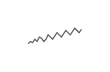
\begin{tikzpicture}[x=0.08em, y=0.08em, line width=0.4pt]
                \draw[FooterGray] (0,3) -- (1,4) -- (2,3.5) -- (3,5) -- (4,4) -- (5,6) -- (6,5.5) -- (7,4) -- (8,5) -- (9,7) -- (10,6) -- (11,5) -- (12,6.5) -- (13,8) -- (14,7) -- (15,6) -- (16,7.5) -- (17,9) -- (18,8) -- (19,7) -- (20,8.5) -- (21,10) -- (22,9) -- (23,8) -- (24,9.5);
            \end{tikzpicture}%
        }%
        \hskip0.5cm%
    }%
    \vskip6pt%
}

%=============================================================================
% PACKAGES
%=============================================================================
\usepackage[utf8]{inputenc}
\DeclareUnicodeCharacter{03B1}{\ensuremath{\alpha}}
\usepackage[T1]{fontenc}
\usepackage{amsmath, amssymb, amsthm}
\usepackage{mathtools}
\usepackage{bm}
\usepackage{tikz}
\usetikzlibrary{arrows.meta, positioning, shapes, calc, decorations.pathreplacing, shadings}
\usepackage{booktabs}
\usepackage{multirow}
\usepackage{array}
\usepackage{graphicx}
\usepackage{animate}
\usepackage{hyperref}
\usepackage{colortbl}
\usepackage{listings}
\lstset{language=Python, basicstyle=\ttfamily\scriptsize, keywordstyle=\color{MainBlue}\bfseries,
  commentstyle=\color{Forest}, stringstyle=\color{Crimson}, breaklines=true,
  frame=none, backgroundcolor=\color{VeryLightGray}, xleftmargin=2mm}
\hypersetup{colorlinks=true, linkcolor=MainBlue, urlcolor=MainBlue}
\graphicspath{{../../logos/}{../../charts/}{../../photos/}}
\usepackage{xcolor}
\hfuzz=2pt  % Suppress tiny overfull warnings (<2pt)
\vfuzz=2pt  % Suppress tiny vertical overfull warnings (<2pt)
% \mathrm in the sans-serif family of the slides (beamer resets \mathrm to the serif family at \begin{document};
% this hook runs after beamer's, so WN, Var, RMSE, ... in formulas match the surrounding text)
% Bold vectors and matrices in the same sans-serif family: \mathbf{A} in sans bold (beamer's own \mathbf came out in
% medium weight), and the bold upright Greek capitals of \boldsymbol / \bm (\bSigma, \bPhi, \boldsymbol{\Theta}) in
% cmss bold: bm.sty fixes its "boldoperators" font when it is loaded (serif cmbx), before beamer switches the
% operators to cmss, so it is reset here.
\AtBeginDocument{%
  \SetMathAlphabet{\mathrm}{normal}{\encodingdefault}{\sfdefault}{\mddefault}{n}%
  \SetMathAlphabet{\mathrm}{bold}{\encodingdefault}{\sfdefault}{bx}{n}%
  \SetMathAlphabet{\mathbf}{normal}{\encodingdefault}{\sfdefault}{bx}{n}%
  \SetMathAlphabet{\mathbf}{bold}{\encodingdefault}{\sfdefault}{bx}{n}%
  \SetSymbolFont{boldoperators}{normal}{OT1}{cmss}{bx}{n}%
  \SetSymbolFont{boldoperators}{bold}{OT1}{cmss}{bx}{n}}

%=============================================================================
% QUANTLET COMMANDS
%   \quantlet{<displayed name>}{<url>}       (generic, compatible with the older TSA decks)
%   \tsaquantlet{Ch_05}{TSA_ch5_garch}       -> https://github.com/danpele/Time-Series-Analysis/tree/main/Quantlets/Ch_05/TSA_ch5_garch
%   \qlurl{<folder>} is defined per chapter by the generator (Quantlets/Ch_NN/<folder>)
%=============================================================================
\newcommand{\tsarepo}{https://github.com/danpele/Time-Series-Analysis}
\newcommand{\tsaqlbase}{https://github.com/danpele/Time-Series-Analysis/tree/main/Quantlets}
\newcommand{\quantlet}[2]{%
    \hfill\href{#2}{%
        \raisebox{-0.15em}{
\includegraphics[height=0.7em]{ql_logo.png}}%
        \textcolor{MainBlue}{\tiny\ #1}%
    }%
}
\newcommand{\tsaquantlet}[2]{\quantlet{\detokenize{#2}}{\tsaqlbase/#1/#2}}

%=============================================================================
% NOTEBOOKS (Google Colab)
%   \colaburl{notebooks/EN/chapter5_seminar_notebook.ipynb} -> the Colab link of a file in the TSA repo
%   \nb: the chapter notebook (each seminar deck redefines it with \renewcommand)
%=============================================================================
\newcommand{\colaburl}[1]{https://colab.research.google.com/github/danpele/Time-Series-Analysis/blob/main/#1}
\newcommand{\nb}{https://colab.research.google.com/github/danpele/Time-Series-Analysis/tree/main/notebooks/EN}
\newcommand{\nbname}{notebooks/EN}

%=============================================================================
% SLIDE HELPERS (used by the generators; the same as in MFM)
%=============================================================================
% local font size for list bodies (the preamble forces \normalsize)
\newcommand{\itemsize}[1]{\setbeamertemplate{itemize/enumerate body begin}{#1}\setbeamertemplate{itemize/enumerate subbody begin}{#1}}
\newcommand{\intitle}[1]{{\hypersetup{urlcolor=white}#1}}   % white links inside coloured title bars
\newcommand{\imgcap}[1]{{\scriptsize #1}\\[0.5mm]}          % caption under a photo
\newcommand{\imgcredit}[2]{{\tiny\color{FooterGray}\href{#1}{#2}}}   % image credit: source URL, author/licence
\newcommand{\aiprompt}[1]{{\ttfamily\color{MainBlue}#1}}     % a prompt to an AI assistant

%=============================================================================
% SEMINARS: student version by default; the instructor wrapper *_solutions.tex sets \solutionstrue
%=============================================================================
\makeatletter\@ifundefined{ifsolutions}{\expandafter\newif\csname ifsolutions\endcsname}{}\makeatother
\newcommand{\solonly}[1]{\ifsolutions #1\fi}
\newcommand{\propsub}{\ifsolutions\else\framesubtitle{\ifdefined\tsalang Rezolvarea se discută la seminar\else Solution discussed in class\fi}\fi}

%=============================================================================
% APPENDIX AND CHAPTER LINKS (latex/appendix_links.py writes the calls; it also re-declares these
% macros before \begin{document}, so the decks compile with or without this preamble block)
%=============================================================================
\providecommand{\tsaapplink}[3]{\hypertarget{#2}{}\hyperlink{#1}{\beamergotobutton{#3}}}
\providecommand{\tsaappback}[2]{\begin{tikzpicture}[remember picture,overlay]\node[anchor=south east] at ([xshift=-3mm,yshift=7mm]current page.south east){\hyperlink{#1}{\beamerreturnbutton{#2}}};\end{tikzpicture}}
\providecommand{\tsachlink}[2]{\href{#1}{#2}}
\providecommand{\tsachlinkt}[2]{\href{#1}{\usebeamercolor[fg]{frametitle}#2}}

%=============================================================================
% QUANTINAR COMMAND: link către un curs Quantinar (subiecte avansate)
%=============================================================================
\newcommand{\quantinar}[2]{%
    \href{#2}{%
        \raisebox{-0.15em}{
\includegraphics[height=0.8em]{qr_logo.png}}%
        \textcolor{MainBlue}{\scriptsize\ #1}%
    }%
}

%=============================================================================
% CUSTOM TITLE PAGE
%=============================================================================
\defbeamertemplate*{title page}{hybrid}[1][]
{
    \vspace{0.2cm}
    % Logos row - top header (with clickable links)
    \begin{center}
        \href{https://www.ase.ro}{
\includegraphics[height=1.0cm]{ase_logo.png}}\hspace{0.3cm}%
        \href{https://theida.net}{
\includegraphics[height=1.0cm]{ida_logo.png}}\hspace{0.3cm}%
        \href{https://blockchain-research-center.com}{
\includegraphics[height=1.0cm]{brc_logo.png}}\hspace{0.3cm}%
        \href{https://www.ai4efin.ase.ro}{
\includegraphics[height=1.0cm]{ai4efin_logo.png}}\hspace{0.3cm}%
        \href{https://ipe.ro/new}{
\includegraphics[height=1.0cm]{acad_logo.png}}\hspace{0.3cm}%
        \href{https://www.digital-finance-msca.com}{
\includegraphics[height=1.0cm]{msca_logo.png}}%
    \end{center}

    \vspace{0.6cm}

    % Main title with Q logos on sides (with clickable links)
    \begin{center}
        \begin{minipage}{0.1\textwidth}
            \centering
            \href{https://quantlet.com}{
\includegraphics[height=1.1cm]{ql_logo.png}}
        \end{minipage}%
        \begin{minipage}{0.78\textwidth}
            \centering
            {\LARGE\bfseries\usebeamercolor[fg]{title}\inserttitle}

            \vspace{0.3cm}

            {\usebeamerfont{subtitle}\usebeamercolor[fg]{title}\insertsubtitle}
        \end{minipage}%
        \begin{minipage}{0.1\textwidth}
            \centering
            \href{https://quantinar.com}{
\includegraphics[height=1.1cm]{qr_logo.png}}
        \end{minipage}
    \end{center}

    \vspace{0.6cm}

    % Authors (left aligned)
    \hspace{0.5cm}{\usebeamerfont{author}\insertauthor}

    \vspace{0.3cm}

    % Institute/Affiliations (left aligned)
    \hspace{0.5cm}\begin{minipage}[t]{0.9\textwidth}
        \raggedright\small\insertinstitute
    \end{minipage}
}

%=============================================================================
% THEOREM ENVIRONMENTS
%=============================================================================
\theoremstyle{definition}
\setbeamertemplate{theorems}[numbered]
\ifdefined\tsalang
\newtheorem{defn}{Definiție}
\newtheorem{thm}{Teoremă}
\newtheorem{prop}{Propoziție}
\newtheorem{rmk}{Observație}
\else
\newtheorem{defn}{Definition}
\newtheorem{thm}{Theorem}
\newtheorem{prop}{Proposition}
\newtheorem{rmk}{Remark}
\fi

%=============================================================================
% CENTRED MINIPAGE (no extra vertical space)
%=============================================================================
\newenvironment{cminipage}[1]{%
    \par\noindent\hfill\begin{minipage}{#1}\ignorespaces
}{%
    \end{minipage}\hfill\null\par
}

%=============================================================================
% CUSTOM COMMANDS
%=============================================================================
\newcommand{\E}{\mathbb{E}}
\newcommand{\Var}{\text{Var}}
\newcommand{\Cov}{\text{Cov}}
\newcommand{\Corr}{\text{Corr}}
\newcommand{\R}{\mathbb{R}}
\newcommand{\N}{\mathbb{N}}
\newcommand{\Z}{\mathbb{Z}}
\newcommand{\B}{\mathbf{B}}
\newcommand{\imark}{\textcolor{MainBlue}{\textbullet}}
\newcommand{\RMSE}{\text{RMSE}}
\newcommand{\MAE}{\text{MAE}}
\newcommand{\MAPE}{\text{MAPE}}

% Boldface vector/matrix commands (VAR, VECM, state space; also used by the older TSA decks)
\newcommand{\bY}{\mathbf{Y}}
\newcommand{\bX}{\mathbf{X}}
\newcommand{\bA}{\mathbf{A}}
\newcommand{\bB}{\mathbf{B}}
\newcommand{\bepsilon}{\boldsymbol{\varepsilon}}
\newcommand{\bSigma}{\boldsymbol{\Sigma}}
\newcommand{\bPhi}{\boldsymbol{\Phi}}
\newcommand{\bGamma}{\boldsymbol{\Gamma}}
\newcommand{\bPi}{\boldsymbol{\Pi}}
\newcommand{\bc}{\mathbf{c}}
\newcommand{\balpha}{\boldsymbol{\alpha}}
\newcommand{\bbeta}{\boldsymbol{\beta}}
\newcommand{\bvarepsilon}{\boldsymbol{\varepsilon}}

% Legacy seminar marks (older TSA seminar decks)
\newcommand{\correct}{\textcolor{Forest}{\checkmark}}
\newcommand{\incorrect}{\textcolor{Crimson}{\texttimes}}


\newcommand{\qlurl}[1]{https://github.com/danpele/Time-Series-Analysis/tree/main/Quantlets/Ch_04/#1}

% Clickable citations (DOIs verified via Crossref)
\newcommand{\refHP}{\href{https://doi.org/10.1007/978-3-031-13584-2}{Huang și Petukhina (2022)}}
\newcommand{\refFPP}{\href{https://otexts.com/fpp3/}{Hyndman și Athanasopoulos (2021)}}
\newcommand{\refFPPsar}{\href{https://otexts.com/fpp3/seasonal-arima.html}{FPP3, secțiunea 9.9}}
\newcommand{\refFPPcomplex}{\href{https://otexts.com/fpp3/complexseasonality.html}{FPP3, secțiunea 12.1}}
\newcommand{\refFPPcv}{\href{https://otexts.com/fpp3/tscv.html}{FPP3, secțiunea 5.10}}
\newcommand{\refFPPdhr}{\href{https://otexts.com/fpp3/dhr.html}{FPP3, secțiunea 10.5}}
\newcommand{\refBD}{\href{https://doi.org/10.1007/978-3-319-29854-2}{Brockwell și Davis (2016)}}
\newcommand{\refBJ}{\href{https://doi.org/10.1002/9781118619193}{Box, Jenkins și Reinsel (2008)}}
\newcommand{\refBoxCox}{\href{https://doi.org/10.1111/j.2517-6161.1964.tb00553.x}{Box și Cox (1964)}}
\newcommand{\refHEGY}{\href{https://doi.org/10.1016/0304-4076(90)90080-D}{Hylleberg, Engle, Granger și Yoo (1990)}}
\newcommand{\refCH}{\href{https://doi.org/10.1080/07350015.1995.10524598}{Canova și Hansen (1995)}}
\newcommand{\refOCSB}{\href{https://doi.org/10.1111/j.1468-0084.1988.mp50004002.x}{Osborn, Chui, Smith și Birchenhall (1988)}}
\newcommand{\refFindley}{\href{https://doi.org/10.1080/07350015.1998.10524743}{Findley et al. (1998)}}
\newcommand{\refLadiray}{\href{https://doi.org/10.1007/978-1-4613-0175-2}{Ladiray și Quenneville (2001)}}
\newcommand{\refDagum}{\href{https://doi.org/10.1007/978-3-319-31822-6}{Dagum și Bianconcini (2016)}}
\newcommand{\refESS}{\href{https://ec.europa.eu/eurostat/web/products-manuals-and-guidelines/w/ks-gq-24-012}{Eurostat (2024)}}
\newcommand{\refMSTL}{\href{https://doi.org/10.1504/ijor.2025.143957}{Bandara, Hyndman și Bergmeir (2025)}}
\newcommand{\refTBATS}{\href{https://doi.org/10.1198/jasa.2011.tm09771}{De Livera, Hyndman și Snyder (2011)}}
\newcommand{\refProphet}{\href{https://doi.org/10.1080/00031305.2017.1380080}{Taylor și Letham (2018)}}
\newcommand{\refDM}{\href{https://doi.org/10.1080/07350015.1995.10524599}{Diebold și Mariano (1995)}}
\newcommand{\refHLN}{\href{https://doi.org/10.1016/S0169-2070(96)00719-4}{Harvey, Leybourne și Newbold (1997)}}
\newcommand{\refTashman}{\href{https://doi.org/10.1016/S0169-2070(00)00065-0}{Tashman (2000)}}
\newcommand{\refBHK}{\href{https://doi.org/10.1016/j.csda.2017.11.003}{Bergmeir, Hyndman și Koo (2018)}}
\newcommand{\refHKo}{\href{https://doi.org/10.1016/j.ijforecast.2006.03.001}{Hyndman și Koehler (2006)}}
\newcommand{\refHK}{\href{https://doi.org/10.18637/jss.v027.i03}{Hyndman și Khandakar (2008)}}
\newcommand{\refBG}{\href{https://doi.org/10.1057/jors.1969.103}{Bates și Granger (1969)}}
\newcommand{\refSW}{\href{https://doi.org/10.1002/for.928}{Stock și Watson (2004)}}
\newcommand{\refSmithWallis}{\href{https://doi.org/10.1111/j.1468-0084.2008.00541.x}{Smith și Wallis (2009)}}
\newcommand{\refWangComb}{\href{https://doi.org/10.1016/j.ijforecast.2022.11.005}{Wang et al. (2023)}}
\newcommand{\refMFour}{\href{https://doi.org/10.1016/j.ijforecast.2019.04.014}{Makridakis, Spiliotis și Assimakopoulos (2020)}}
\newcommand{\refGEF}{\href{https://doi.org/10.1016/j.ijforecast.2016.02.001}{Hong et al. (2016)}}
\newcommand{\refPetro}{\href{https://doi.org/10.1016/j.ijforecast.2021.11.001}{Petropoulos et al. (2022)}}
\newcommand{\refLB}{\href{https://doi.org/10.1093/biomet/65.2.297}{Ljung și Box (1978)}}

\title[Serii de timp]{Serii de timp}
\subtitle{Capitolul 4: Sezonalitate și prognoză: SARIMA, TBATS, Prophet}
\author[D.T. Pele]{Daniel Traian PELE}
\institute{Academia de Studii Economice din București\\
IDA Institute Digital Assets\\
Blockchain Research Center\\
AI4EFin Artificial Intelligence for Energy Finance\\
Academia Română, Institutul de Prognoză Economică\\
MSCA Digital Finance}
\date{}

%=============================================================================
\providecommand{\tsaapplink}[3]{\hypertarget{#2}{}\hyperlink{#1}{\beamergotobutton{#3}}}  % APPLINKS-MACROS
\providecommand{\tsaappback}[2]{\begin{tikzpicture}[remember picture,overlay]\node[anchor=south east] at ([xshift=-3mm,yshift=7mm]current page.south east){\hyperlink{#1}{\beamerreturnbutton{#2}}};\end{tikzpicture}}  % APPLINKS-MACROS
\providecommand{\tsachlink}[2]{\href{#1}{#2}}  % APPLINKS-MACROS
\providecommand{\tsachlinkt}[2]{\href{#1}{\usebeamercolor[fg]{frametitle}#2}}  % APPLINKS-MACROS
\begin{document}
%=============================================================================

{
\setbeamertemplate{headline}{}
\setbeamertemplate{footline}{}
\begin{frame}[noframenumbering]
    \titlepage
\end{frame}
}
% BEGIN-ACRONYMS (generat de latex/acronyms.py; nu editati manual)
\begin{frame}{Acronime folosite în acest material (1/2)}
\setbeamertemplate{itemize/enumerate body begin}{\tiny}
\begin{columns}[T]
\begin{column}{0.49\textwidth}
\begin{itemize}\setlength{\itemsep}{0pt}
    \item \textbf{ACF}: Autocorrelation Function (funcția de autocorelație)
    \item \textbf{AI}: Artificial Intelligence (inteligență artificială)
    \item \textbf{AIC}: Akaike Information Criterion (criteriul informațional Akaike)
    \item \textbf{AR}: AutoRegressive (model) — model autoregresiv
    \item \textbf{ARCH}: AutoRegressive Conditional Heteroskedasticity (heteroscedasticitate condiționată autoregresivă)
    \item \textbf{ARIMA}: AutoRegressive Integrated Moving Average (model) — model autoregresiv integrat cu medie mobilă
    \item \textbf{ARMA}: AutoRegressive Moving Average (model) — model autoregresiv cu medie mobilă
    \item \textbf{BIC}: Bayesian Information Criterion (criteriul informațional bayesian (Schwarz))
    \item \textbf{CA}: Calendar Adjusted (ajustat pentru efectele de calendar)
    \item \textbf{DHR}: Dynamic Harmonic Regression (regresie armonică dinamică)
    \item \textbf{DM}: Diebold–Mariano (test) — testul Diebold–Mariano de comparare a prognozelor
    \item \textbf{ENTSO-E}: European Network of Transmission System Operators for Electricity (rețeaua europeană a operatorilor de transport și de sistem pentru energie electrică)
    \item \textbf{ETS}: Error, Trend, Seasonality (exponential smoothing state space models) — eroare, trend, sezonalitate (modele de netezire exponențială)
\end{itemize}
\end{column}
\begin{column}{0.49\textwidth}
\begin{itemize}\setlength{\itemsep}{0pt}
    \item \textbf{GARCH}: Generalised AutoRegressive Conditional Heteroskedasticity (heteroscedasticitate condiționată autoregresivă generalizată)
    \item \textbf{GW}: Gigawatt (gigawatt)
    \item \textbf{HEGY}: Hylleberg–Engle–Granger–Yoo (seasonal unit-root test) — testul Hylleberg–Engle–Granger–Yoo de rădăcină unitară sezonieră
    \item \textbf{HLN}: Harvey–Leybourne–Newbold (small-sample correction of the DM test) — corecția Harvey–Leybourne–Newbold a testului DM pentru eșantioane mici
    \item \textbf{IAPC}: Indicele armonizat al prețurilor de consum
    \item \textbf{KPSS}: Kwiatkowski–Phillips–Schmidt–Shin (test) — testul de staționaritate Kwiatkowski–Phillips–Schmidt–Shin
    \item \textbf{LB}: Ljung–Box (test) — testul de autocorelație Ljung–Box
    \item \textbf{MA}: Moving Average (medie mobilă)
    \item \textbf{MAE}: Mean Absolute Error (eroarea absolută medie)
    \item \textbf{MAPE}: Mean Absolute Percentage Error (eroarea procentuală absolută medie)
    \item \textbf{MASE}: Mean Absolute Scaled Error (eroarea absolută medie scalată)
    \item \textbf{MSTL}: Multiple Seasonal-Trend decomposition using Loess (descompunerea sezonier-trend cu mai multe perioade, prin Loess)
    \item \textbf{MW}: Megawatt (megawatt)
\end{itemize}
\end{column}
\end{columns}
\end{frame}
\begin{frame}{Acronime folosite în acest material (2/2)}
\setbeamertemplate{itemize/enumerate body begin}{\tiny}
\begin{columns}[T]
\begin{column}{0.49\textwidth}
\begin{itemize}\setlength{\itemsep}{0pt}
    \item \textbf{NSA}: Not Seasonally Adjusted (neajustat sezonier)
    \item \textbf{OCSB}: Osborn–Chui–Smith–Birchenhall (seasonal unit-root test) — testul Osborn–Chui–Smith–Birchenhall de rădăcină unitară sezonieră
    \item \textbf{PACF}: Partial AutoCorrelation Function (funcția de autocorelație parțială)
    \item \textbf{PIB}: Produsul intern brut
    \item \textbf{RMSE}: Root Mean Squared Error (rădăcina erorii pătratice medii)
    \item \textbf{SARIMA}: Seasonal ARIMA (model) — model ARIMA sezonier
    \item \textbf{SCA}: Seasonally and Calendar Adjusted (ajustat sezonier și pentru efectele de calendar)
    \item \textbf{SEATS}: Signal Extraction in ARIMA Time Series (extragerea semnalului din serii de timp ARIMA)
    \item \textbf{STL}: Seasonal and Trend decomposition using Loess (descompunerea în sezonalitate și trend cu Loess)
    \item \textbf{TBATS}: Trigonometric seasonality, Box–Cox, ARMA errors, Trend, Seasonal components (model) — model cu sezonalitate trigonometrică, transformare Box–Cox, erori ARMA, trend și componente sezoniere
    \item \textbf{TRAMO-SEATS}: Time series Regression with ARIMA noise, Missing values and Outliers; Signal Extraction in ARIMA Time Series (metodă de ajustare sezonieră pe baza modelelor ARIMA)
    \item \textbf{TVA}: Taxa pe valoarea adăugată
    \item \textbf{UE}: Uniunea Europeană
\end{itemize}
\end{column}
\begin{column}{0.49\textwidth}
\begin{itemize}\setlength{\itemsep}{0pt}
    \item \textbf{US}: United States (Statele Unite ale Americii)
    \item \textbf{UTC}: Coordinated Universal Time (Temps Universel Coordonné) — timpul universal coordonat
\end{itemize}
\end{column}
\end{columns}
\end{frame}
% END-ACRONYMS

\begin{frame}{Întrebarea de azi și traseul}
\itemsize{\footnotesize}
\begin{itemize}
    \item \textbf{Întrebarea}: multe serii economice repetă un tipar în fiecare an, săptămînă sau zi; cum modelăm acest tipar, cum prognozăm cu el și cum decidem care prognoză este mai bună?
    \begin{itemize}
        \item trei răspunsuri: \textbf{eliminăm} tiparul prin diferențiere (SARIMA), îl \textbf{modelăm} cu regresori (termeni Fourier, TBATS, Prophet) sau îl \textbf{scoatem} din date (ajustarea sezonieră)
    \end{itemize}
    \item \textbf{Traseul} capitolului
    \begin{itemize}
        \item diferențe sezoniere și rădăcini unitare sezoniere (HEGY, Canova--Hansen, OCSB)
        \item SARIMA$(p,d,q)(P,D,Q)_s$: identificare, estimare, diagnosticare, prognoze; modelul airline și PIB-ul României
        \item ajustarea sezonieră în practică (X-13ARIMA-SEATS, Eurostat), termeni Fourier și efecte de calendar (Paștele ortodox)
        \item sezonalitatea multiplă a consumului de electricitate: MSTL, regresia armonică dinamică, TBATS, Prophet
        \item evaluarea prognozelor (validare încrucișată pentru serii de timp, testul Diebold--Mariano) și combinarea prognozelor
    \end{itemize}
    \item Capitolul se sprijină pe \tsachlink{https://danpele.github.io/Time-Series-Analysis/RO/Cursuri/capitol0_introducere.pdf}{Capitolul 0} (componente, Holt--Winters, MASE) și pe \tsachlink{https://danpele.github.io/Time-Series-Analysis/RO/Cursuri/capitol2_modele_arma.pdf}{Capitolele 2}--\tsachlink{https://danpele.github.io/Time-Series-Analysis/RO/Cursuri/capitol3_radacini_unitare_modele_arima.pdf}{3} (ARMA, rădăcini unitare, ARIMA): aceleași idei, la lagul sezonier $s$
    \item Seminarul 4 are loc înaintea acestui curs: dă formulele; aici le deducem și le aplicăm pe date
\end{itemize}
\end{frame}

\begin{frame}{Rezultatele învățării}
\itemsize{\small}
\begin{itemize}
    \item Recunoașteți sezonalitatea deterministă și pe cea stochastică și alegeți diferențierea sezonieră cu testele HEGY, Canova--Hansen și OCSB
    \item Scrieți, identificați, estimați, verificați și prognozați un model SARIMA$(p,d,q)(P,D,Q)_s$ și dezvoltați polinoamele lui
    \item Interpretați corect seriile oficiale ajustate sezonier și neajustate și explicați ce face X-13ARIMA-SEATS
    \item Modelați efectele de calendar (zile lucrătoare, Paștele ortodox) și sezonalitatea multiplă cu termeni Fourier, MSTL, TBATS și Prophet
    \item Comparați prognozele cu validarea încrucișată pentru serii de timp, MASE și testul Diebold--Mariano și combinați-le
\end{itemize}
\end{frame}

\begin{frame}{Bibliografie și instrumente}
\itemsize{\small}
\begin{itemize}
    \item Manual: \refHP, cap.~4--5 (modele ARIMA și modele nestaționare)
    \begin{itemize}
        \item manual însoțitor, gratuit online: \refFPP, cap.~9 (\refFPPsar), cap.~10 (\refFPPdhr), cap.~12 (\refFPPcomplex) și cap.~13
    \end{itemize}
    \item Lucrarea clasică: \refBJ, cap.~9 (modele sezoniere); ajustarea sezonieră: \refLadiray, \refDagum, \refESS
    \item Quantlet-urile Python ale capitolului: \href{https://github.com/danpele/Time-Series-Analysis/tree/main/Quantlets/Ch_04}{Quantlets/Ch\_04}
    \begin{itemize}
        \item \texttt{statsmodels} (\texttt{SARIMAX}, \texttt{MSTL}, \texttt{ExponentialSmoothing}); pachetele opționale \texttt{tbats} și \texttt{prophet}
    \end{itemize}
    \item Notebook-ul cursului: \href{\colaburl{notebooks/EN/chapter4_lecture_notebook.ipynb}}{deschideți în Google Colab}
    \item Curs video: \quantinar{Applied Time Series Analysis with Python}{https://quantinar.com/course/137/applied-time-series-analysis-with-python}
\end{itemize}
\end{frame}


%=============================================================================
\section{Sezonalitatea în datele economice}
%=============================================================================

\begin{frame}{Sezonalitatea: definiție și surse}
\itemsize{\small}
\begin{itemize}
    \item \textbf{Sezonalitatea}: un tipar care se repetă cu o \textbf{perioadă} $s$ fixă și cunoscută (observații pe ciclu)
    \begin{itemize}
        \item $s = 4$ (trimestre), $s = 12$ (luni), $s = 7$ (zile într-o săptămînă), $s = 24$ și $s = 168$ (ore într-o zi și într-o săptămînă)
        \item spre deosebire de \textbf{ciclu}, a cărui lungime este neregulată și necunoscută (\tsachlink{https://danpele.github.io/Time-Series-Analysis/RO/Cursuri/capitol0_introducere.pdf}{Capitolul 0})
    \end{itemize}
    \item \textbf{Surse}
    \begin{itemize}
        \item vremea: încălzirea iarna, litoralul în august, recoltele
        \item calendarul: zilele lucrătoare, sărbătorile legale, \textbf{sărbătorile mobile}, precum Paștele ortodox
        \item instituțiile și obiceiurile: anul școlar, termenele fiscale, primele de sfîrșit de an, săptămîna de lucru
    \end{itemize}
    \item \textbf{Aditivă} ($y_t = T_t + S_t + R_t$) sau \textbf{multiplicativă} ($y_t = T_tS_tR_t$, aditivă după logaritmare): \tsachlink{https://danpele.github.io/Time-Series-Analysis/RO/Cursuri/capitol0_introducere.pdf}{Capitolul 0}; aici lucrăm cu logaritmi cînd amplitudinea crește cu nivelul
\end{itemize}
\end{frame}

\begin{frame}{Sezonalitatea în șase serii din România}
\itemsize{\footnotesize}
\begin{center}
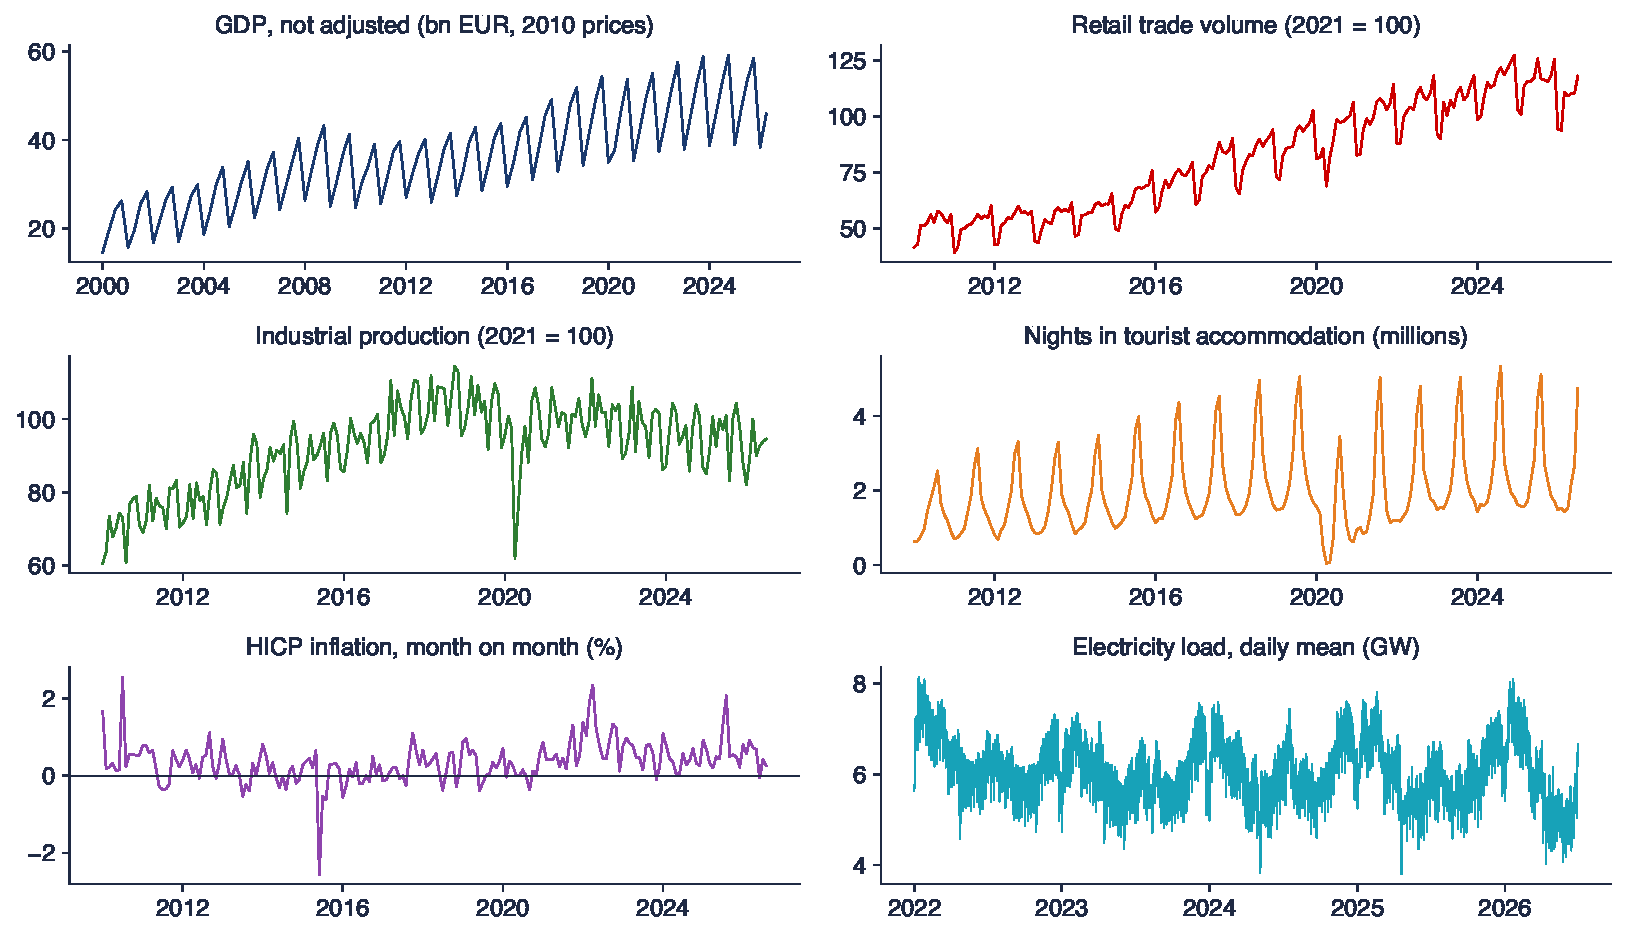
\includegraphics[width=0.97\textwidth,height=0.70\textheight,keepaspectratio]{tsa_ch4_series.pdf}
\end{center}
\vspace{-0.25cm}
\begin{itemize}
    \item Eurostat: PIB (trimestrial, neajustat), comerțul cu amănuntul, producția industrială, înnoptările turistice, IAPC; ENTSO-E: consumul zilnic de electricitate
\end{itemize}
\quantlet{TSA\_ch4\_seasonal\_data}{\qlurl{TSA_ch4_seasonal_data}}
\end{frame}

\begin{frame}{Interpretarea celor șase serii}
\itemsize{\footnotesize}
\begin{itemize}
    \item PIB: media trimestrului 4 este cu 57\% peste media trimestrului 1 (2000--2026); amplitudinea crește cu nivelul: multiplicativă, folosim logaritmi
    \begin{itemize}
        \item mediile trimestriale (mld. EUR, prețuri 2010): 27{,}8; 33{,}6; 39{,}5; 43{,}6: construcțiile și agricultura în T2--T3
    \end{itemize}
    \item Turismul: august are de 3{,}7 ori mai multe înnoptări decît ianuarie (2015--2019); restricțiile din 2020 (lockdown) întrerup tiparul
    \item IAPC: inflația lunară este mai mică în iunie (în medie \ensuremath{-}0{,}37\%, 2010--2019, alimentele proaspete) și mai mare în octombrie (0{,}49\%)
    \item Electricitatea: două tipare simultan, săptămîna (oscilația deasă) și anul (vîrfurile de iarnă): \textbf{sezonalitate multiplă}, secțiunea 8
\end{itemize}
\end{frame}

\begin{frame}{Graficul sezonier și graficul pe subserii}
\itemsize{\footnotesize}
\begin{center}
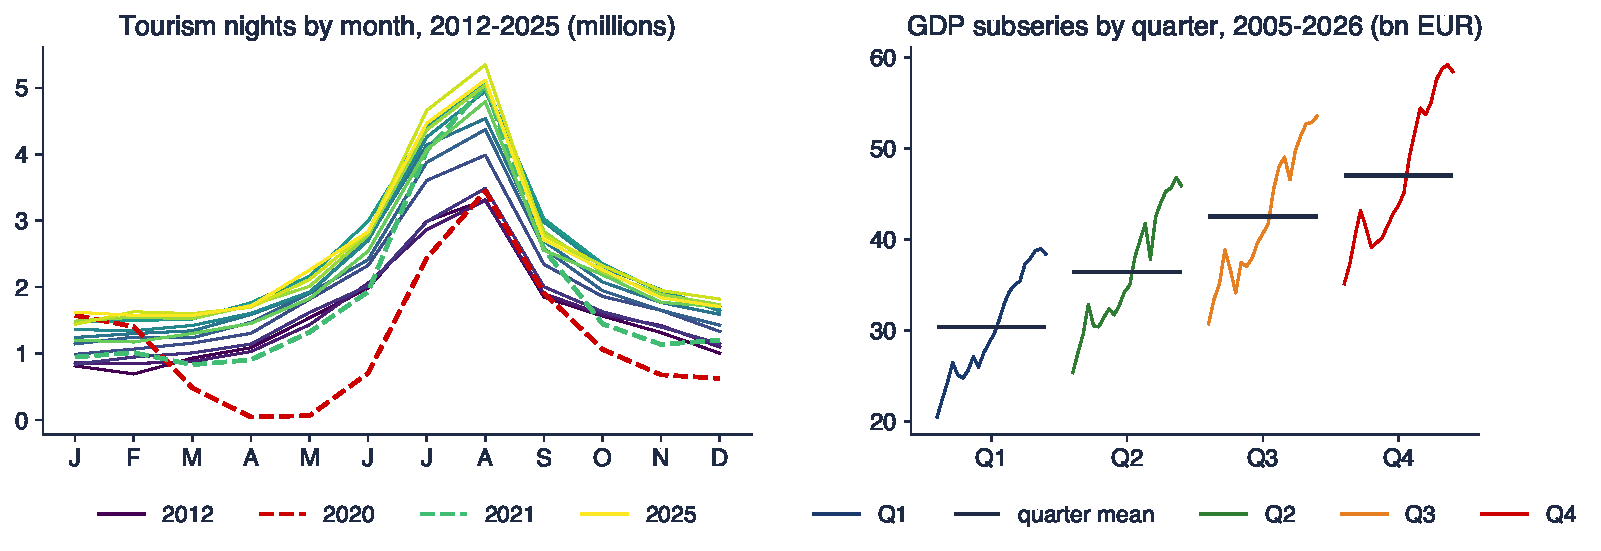
\includegraphics[width=0.97\textwidth,height=0.62\textheight,keepaspectratio]{tsa_ch4_seasonal_plot.pdf}
\end{center}
\vspace{-0.25cm}
\begin{itemize}
    \item Stînga: o linie pentru fiecare an (graficul sezonier); dreapta: fiecare trimestru al PIB-ului urmărit de-a lungul anilor, cu media lui (graficul pe subserii)
\end{itemize}
\quantlet{TSA\_ch4\_seasonal\_data}{\qlurl{TSA_ch4_seasonal_data}}
\end{frame}

\begin{frame}{Interpretarea graficelor sezoniere}
\itemsize{\footnotesize}
\begin{columns}[T]
\begin{column}{0.58\textwidth}
\begin{itemize}
    \item Turismul: aceeași formă în fiecare an, un vîrf vara și un minim iarna
    \begin{itemize}
        \item 2019: 5{,}06 milioane de înnoptări în august, 1{,}47 milioane în ianuarie
        \item aprilie 2020: 0{,}045 milioane (1{,}76 milioane în aprilie 2019): o valoare aberantă, nu un sezon nou
    \end{itemize}
    \item Subseriile PIB: toate cele patru trimestre cresc paralel
    \begin{itemize}
        \item o formă sezonieră stabilă peste un trend comun
        \item dacă liniile s-ar intersecta, tiparul sezonier s-ar schimba: sezonalitate stochastică (secțiunea următoare)
    \end{itemize}
\end{itemize}
\end{column}
\begin{column}{0.38\textwidth}
\centering
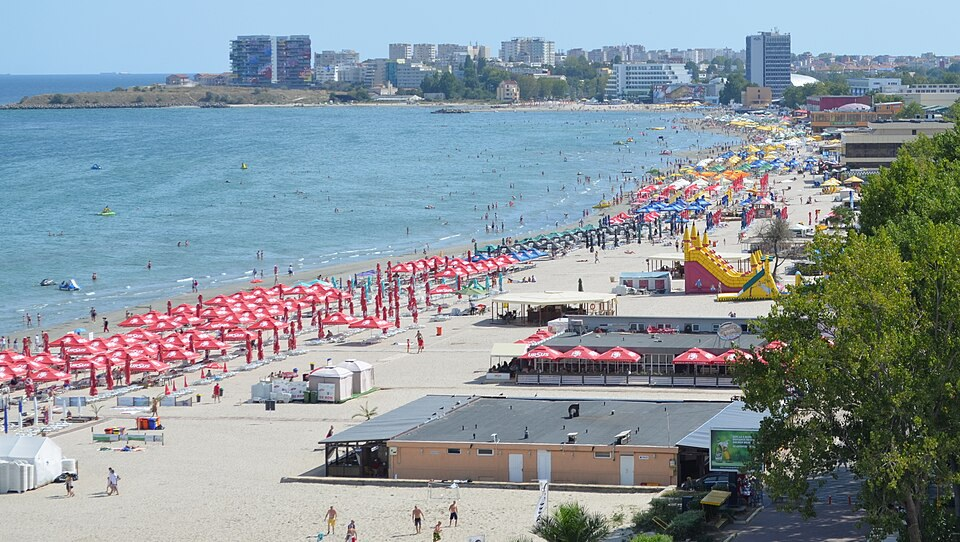
\includegraphics[height=0.36\textheight]{ch4_mamaia_2013.jpg}\\[1mm]
\imgcap{Mamaia, pe litoralul Mării Negre, septembrie 2013}
\imgcredit{https://commons.wikimedia.org/wiki/File:Mamaia_Beach_(September_2013).JPG}{Foto: Razvan Socol (2013); CC BY-SA 4.0; Wikimedia Commons}
\end{column}
\end{columns}
\end{frame}

\begin{frame}{Recapitulare: sezonalitatea în datele economice}
\itemsize{\small}
\begin{itemize}
    \item Sezonalitatea se repetă cu o perioadă cunoscută $s$; ciclul nu
    \item Vremea, calendarul și instituțiile o creează; sărbătorile mobile o mută între luni
    \item PIB-ul, turismul, inflația și consumul de electricitate din România sînt toate sezoniere; electricitatea are mai multe perioade simultan
    \item Graficele sezoniere și pe subserii arată dacă tiparul este stabil
\end{itemize}
\end{frame}


%=============================================================================
\section{Diferențierea sezonieră și rădăcinile unitare sezoniere}
%=============================================================================

\begin{frame}{Diferența sezonieră}
\itemsize{\small}
\begin{itemize}
    \item \textbf{Diferența sezonieră}: $\Delta_s y_t = (1 - L^s)y_t = y_t - y_{t-s}$
    \begin{itemize}
        \item cu logaritmi: $100\,\Delta_4\ln Y_t$ = creșterea față de același trimestru al anului anterior, în \%
    \end{itemize}
    \item Un tipar sezonier \textbf{fix} $S_t = S_{t-s}$ plus un trend liniar: $y_t = a + bt + S_t + \varepsilon_t$
    \begin{itemize}
        \item $a$: termenul liber; $b$: panta trendului; $S_t$: efectul sezonier al perioadei $t$
        \item $\Delta_s y_t = bs + \varepsilon_t - \varepsilon_{t-s}$: $\Delta_s$ elimină tiparul și transformă trendul într-o constantă
        \item dar creează termenul MA neinvertibil $\varepsilon_t - \varepsilon_{t-s}$: \textbf{supradiferențiere sezonieră} (ca în \tsachlink{https://danpele.github.io/Time-Series-Analysis/RO/Cursuri/capitol3_radacini_unitare_modele_arima.pdf}{Capitolul 3})
    \end{itemize}
    \item $\Delta\Delta_s = (1 - L)(1 - L^s) = 1 - L - L^s + L^{s+1}$: necesar cînd și trendul este stochastic
    \begin{itemize}
        \item ordinea celor două diferențe nu contează: operatorii comută
    \end{itemize}
\end{itemize}
\end{frame}

\begin{frame}{Sezonalitatea deterministă și sezonalitatea stochastică}
\itemsize{\small}
\begin{itemize}
    \item \textbf{Deterministă}: $y_t = \sum_{j=1}^{s}\gamma_jD_{jt} + u_t$, cu $D_{jt} = 1$ în sezonul $j$ și $u_t$ staționar
    \begin{itemize}
        \item mediile sezoniere $\gamma_j$ nu se schimbă niciodată; instrumentul potrivit: variabile dummy sezoniere sau termeni Fourier (secțiunea 7)
    \end{itemize}
    \item \textbf{Stochastică}: \textbf{mersul aleator sezonier} $y_t = y_{t-s} + \varepsilon_t$
    \begin{itemize}
        \item fiecare sezon este propriul mers aleator: $s$ mersuri aleatoare separate, intercalate
        \item $\mathrm{Var}(y_t)$ crește nelimitat; tiparul se deplasează, iar „vara poate deveni iarnă”
        \item instrumentul potrivit: diferența sezonieră $\Delta_s$
    \end{itemize}
    \item Alegerea contează: diferențierea unui tipar determinist duce la supradiferențiere; modelarea unuia stochastic cu variabile dummy lasă o rădăcină unitară în reziduuri
\end{itemize}
\end{frame}

\begin{frame}{Rădăcinile lui $1 - z^s$: rădăcini unitare sezoniere}
\itemsize{\footnotesize}
\begin{center}
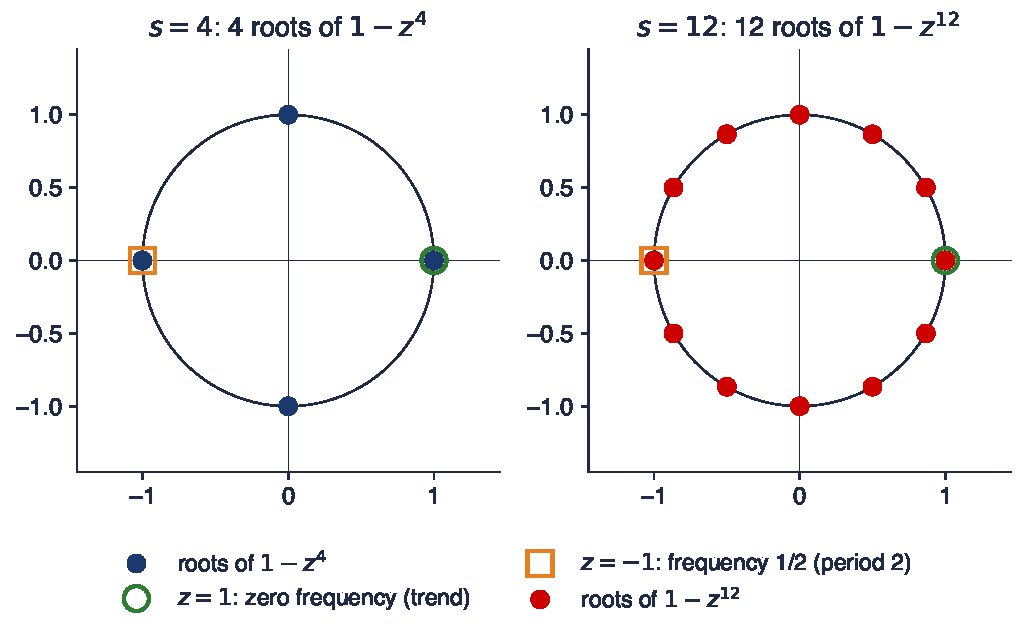
\includegraphics[width=0.97\textwidth,height=0.58\textheight,keepaspectratio]{tsa_ch4_unit_circle.pdf}
\end{center}
\vspace{-0.25cm}
\begin{itemize}
    \item $1 - z^4 = (1 - z)(1 + z)(1 + z^2)$: rădăcinile $1$, $-1$, $\pm i$, toate pe cercul unitate
\end{itemize}
\quantlet{TSA\_ch4\_seasonal\_roots}{\qlurl{TSA_ch4_seasonal_roots}}
\end{frame}

\begin{frame}{Interpretarea rădăcinilor sezoniere}
\itemsize{\small}
\begin{itemize}
    \item $\Delta_s$ impune simultan $s$ rădăcini unitare, cîte una pentru fiecare \textbf{frecvență} $k/s$, $k = 0, \dots, s - 1$
    \begin{itemize}
        \item trimestrial: $z = 1$ (frecvența 0, trendul), $z = -1$ (o jumătate de ciclu pe trimestru: perioada de 2 trimestre), $z = \pm i$ (perioada de 4 trimestre: ciclul anual)
    \end{itemize}
    \item O serie poate avea unele dintre aceste rădăcini și nu pe altele: atunci $\Delta_4$ supradiferențiază la frecvențele de care nu are nevoie
    \item Testele de rădăcină unitară sezonieră întreabă, frecvență cu frecvență, ce rădăcini sînt prezente: testul HEGY (slide-urile următoare)
\end{itemize}
\end{frame}

\begin{frame}{PIB-ul României: diferențe obișnuite și sezoniere}
\itemsize{\footnotesize}
\begin{center}
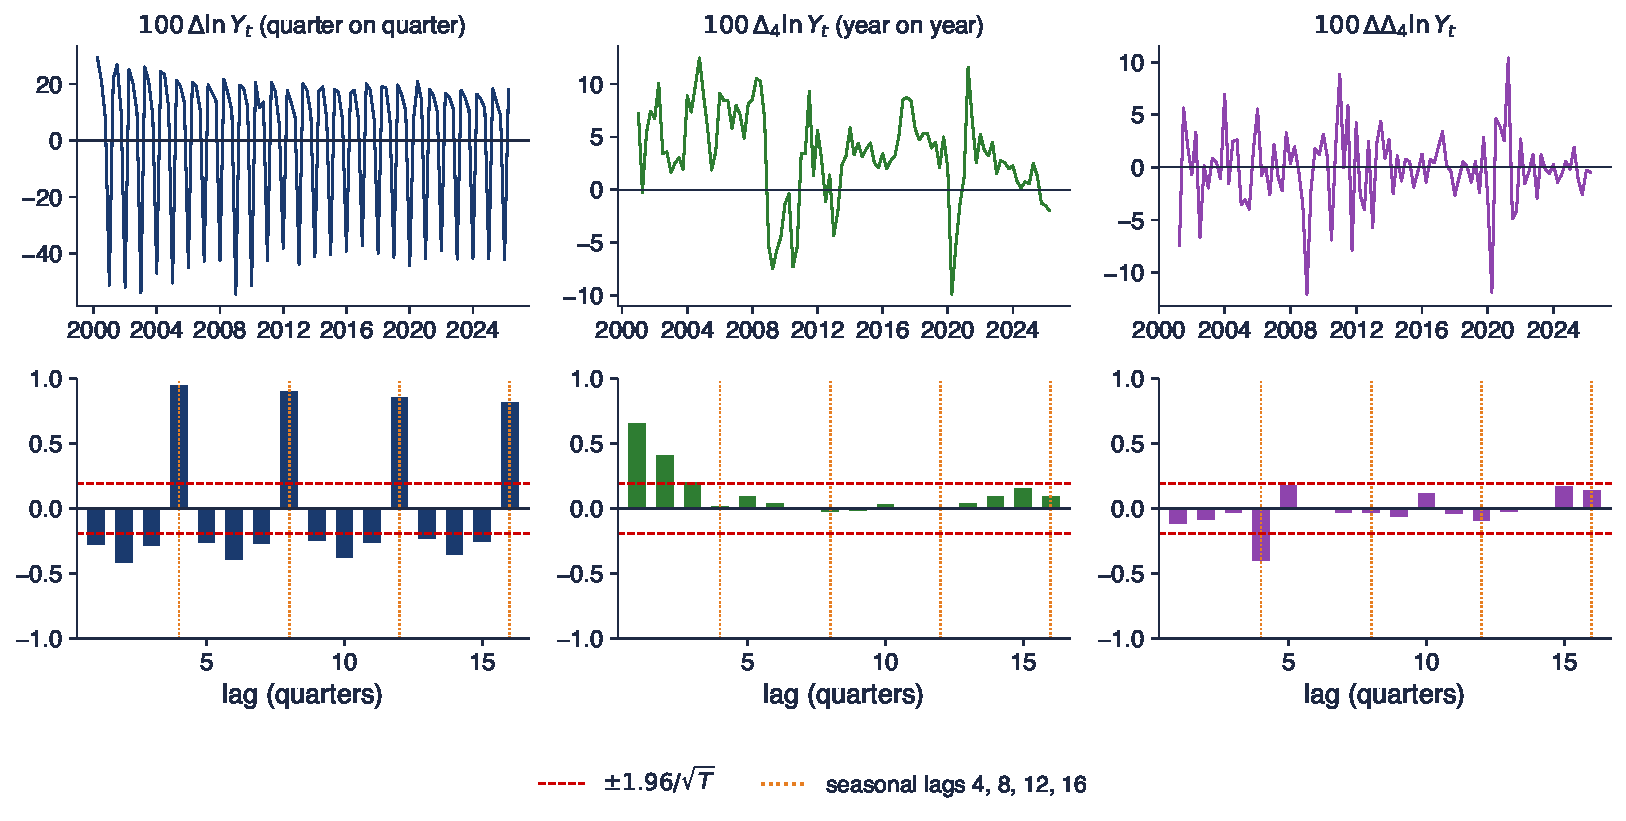
\includegraphics[width=0.97\textwidth,height=0.66\textheight,keepaspectratio]{tsa_ch4_gdp_diff.pdf}
\end{center}
\vspace{-0.25cm}
\begin{itemize}
    \item $\ln$ din PIB-ul real neajustat, 106 de trimestre pînă în T2 2026; sus: trei transformări; jos: ACF de selecție pînă la 16 trimestre
\end{itemize}
\quantlet{TSA\_ch4\_seasonal\_roots}{\qlurl{TSA_ch4_seasonal_roots}}
\end{frame}

\begin{frame}{Interpretarea celor trei transformări}
\itemsize{\footnotesize}
\begin{itemize}
    \item $\Delta\ln Y$: dominată de sezon: ACF $0{,}95$ la lagul 4 și $0{,}90$ la lagul 8, cu o descreștere foarte lentă; abaterea standard 26{,}5\%
    \begin{itemize}
        \item analogul sezonier al descreșterii lente a ACF pentru un mers aleator (\tsachlink{https://danpele.github.io/Time-Series-Analysis/RO/Cursuri/capitol3_radacini_unitare_modele_arima.pdf}{Capitolul 3})
    \end{itemize}
    \item $\Delta_4\ln Y$ (creșterea anuală): abaterea standard 4{,}4\%; ACF $0{,}66$ la lagul 1, $0{,}01$ la lagul 4: un tipar de tip AR
    \item $\Delta\Delta_4\ln Y$: ACF $\ensuremath{-}0{,}11$ la lagul 1 și $\ensuremath{-}0{,}40$ la lagul 4 (banda $\pm 0{,}20$)
    \begin{itemize}
        \item o singură valoare negativă semnificativă la lagul sezonier: un MA(1) sezonier, semnătura modelului airline (secțiunea 3)
    \end{itemize}
\end{itemize}
\end{frame}

\begin{frame}{Testul HEGY}
\itemsize{\footnotesize}
\begin{columns}[T]
\begin{column}{0.64\textwidth}
\begin{itemize}
    \item \refHEGY: o singură regresie testează fiecare rădăcină sezonieră a unei serii trimestriale
    \begin{itemize}
        \item filtre: $y_{1t} = (1 + L + L^2 + L^3)y_t$, $y_{2t} = -(1 - L + L^2 - L^3)y_t$, $y_{3t} = -(1 - L^2)y_t$
    \end{itemize}
    \item $\Delta_4y_t = \pi_1y_{1,t-1} + \pi_2y_{2,t-1} + \pi_3y_{3,t-2} + \pi_4y_{3,t-1} + \text{termeni determiniști} + \text{laguri ale lui } \Delta_4y_t + \varepsilon_t$
    \begin{itemize}
        \item $y_{1t}, y_{2t}, y_{3t}$: seria filtrată astfel încît fiecare să păstreze o singură frecvență sezonieră; $\pi_k$: coeficientul fiecărei frecvențe
        \item $H_0$: $\pi_1 = 0$ (rădăcina $1$), test $t$; $\pi_2 = 0$ (rădăcina $-1$), test $t$; $\pi_3 = \pi_4 = 0$ (rădăcinile $\pm i$), test $F$
        \item distribuții nestandard, ca la Dickey--Fuller: valori critice din tabele sau prin simulare
    \end{itemize}
    \item Respingerea tuturor celor trei: nu este nevoie de diferențiere sezonieră; nicio respingere: $\Delta_4$ este justificată
\end{itemize}
\end{column}
\begin{column}{0.32\textwidth}
\centering
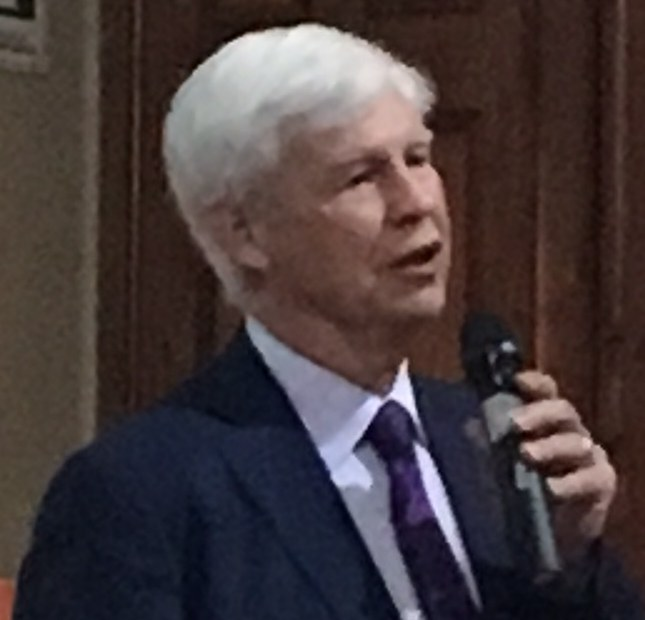
\includegraphics[height=0.40\textheight]{ch4_robert_engle_2017.jpg}\\[1mm]
\imgcap{Robert Engle, coautor al testului HEGY, 2017}
\imgcredit{https://commons.wikimedia.org/wiki/File:Robert_Engle_SantiagoWEAI2017.png}{Foto: Econterms (2017); CC BY-SA 4.0; Wikimedia Commons}
\end{column}
\end{columns}
\end{frame}

\begin{frame}{Testele Canova--Hansen și OCSB}
\itemsize{\small}
\begin{itemize}
    \item \textbf{Canova--Hansen} (\refCH): ipoteza nulă este sezonalitatea \textbf{stabilă} (deterministă)
    \begin{itemize}
        \item analogul sezonier al testului KPSS (\tsachlink{https://danpele.github.io/Time-Series-Analysis/RO/Cursuri/capitol3_radacini_unitare_modele_arima.pdf}{Capitolul 3}): respingerea înseamnă că tiparul se schimbă în timp
    \end{itemize}
    \item \textbf{OCSB} (\refOCSB): ipoteza nulă este o rădăcină unitară sezonieră; o regresie a lui $\Delta\Delta_s y_t$ pe $\Delta_s y_{t-1}$ și $\Delta y_{t-s}$
    \begin{itemize}
        \item testul sezonier implicit al funcției \texttt{auto\_arima} din pachetul Python \texttt{pmdarima} (\texttt{nsdiffs})
    \end{itemize}
    \item Ca în \tsachlink{https://danpele.github.io/Time-Series-Analysis/RO/Cursuri/capitol3_radacini_unitare_modele_arima.pdf}{Capitolul 3}: testele cu ipoteze nule opuse răspund la întrebări diferite; folosiți-le împreună
    \begin{itemize}
        \item și priviți datele: graficele sezoniere, ACF la lagurile $s, 2s, 3s$ și mărimea lui $\hat\Theta$ după $\Delta_s$ ($\hat\Theta \approx -1$ semnalează supradiferențierea)
    \end{itemize}
\end{itemize}
\end{frame}

\begin{frame}{Teste de rădăcină unitară sezonieră pe date din România}
\itemsize{\scriptsize}
\begin{center}
\scriptsize
\begin{tabular}{lrrr}
\toprule
\textbf{HEGY}, $\ln$ PIB, 2000--2019 & statistica & valoarea critică 5\% & decizia \\
\midrule
$t(\pi_1)$, rădăcina $1$ & $\ensuremath{-}1{,}97$ & $\ensuremath{-}3{,}39$ & nu se respinge \\
$t(\pi_2)$, rădăcina $-1$ & $\ensuremath{-}2{,}19$ & $\ensuremath{-}2{,}77$ & nu se respinge \\
$F(\pi_3, \pi_4)$, rădăcinile $\pm i$ & $6{,}12$ & $6{,}64$ & nu se respinge \\
\bottomrule
\end{tabular}
\end{center}
\begin{center}
\scriptsize
\begin{tabular}{lccc}
\toprule
\textbf{Seria} (logaritmi, 2005--2019) & $D$ după OCSB & $D$ după Canova--Hansen & $d$ după KPSS \\
\midrule
PIB (trimestrial) & 1 & 0 & 1 \\
Comerțul cu amănuntul & 0 & 0 & 1 \\
Producția industrială & 0 & 0 & 1 \\
Înnoptări turistice & 0 & 0 & 1 \\
IAPC & 0 & 0 & 2 \\
\bottomrule
\end{tabular}
\end{center}
\begin{itemize}
    \item HEGY: constantă, variabile dummy sezoniere și trend, 1 lag al lui $\Delta_4y$ (AIC), $n = 75$; valori critice din 4\,000 de simulări ale lui $\Delta_4y_t = \varepsilon_t$
    \item Interpretare: pentru PIB, HEGY și OCSB susțin $\Delta_4$, în timp ce Canova--Hansen nu respinge un tipar stabil; cu 20 de ani de date trimestriale ambele perspective se potrivesc, deci folosim $\Delta_4$ și lăsăm $\hat\Theta$ să arate cît de stabil este tiparul (secțiunea 5)
    \item Seriile lunare: ambele teste aleg $D = 0$, un tipar stabil; IAPC are nevoie de $d = 2$ în logaritmi: inflația însăși este aproape de o rădăcină unitară (\tsachlink{https://danpele.github.io/Time-Series-Analysis/RO/Cursuri/capitol3_radacini_unitare_modele_arima.pdf}{Capitolul 3})
\end{itemize}
\end{frame}

\begin{frame}{Recapitulare: diferențierea sezonieră și rădăcinile unitare sezoniere}
\itemsize{\small}
\begin{itemize}
    \item $\Delta_s = 1 - L^s$ are $s$ rădăcini unitare pe cerc, cîte una pentru fiecare frecvență sezonieră
    \item Sezonalitatea deterministă: variabile dummy sau termeni Fourier; sezonalitatea stochastică: $\Delta_s$
    \item HEGY și OCSB testează rădăcinile unitare sezoniere; Canova--Hansen testează un tipar stabil
    \item PIB-ul României: $\Delta\Delta_4\ln Y$ lasă o singură valoare semnificativă la lagul 4, un MA sezonier
\end{itemize}
\end{frame}


%=============================================================================
\section{Modele SARIMA}
%=============================================================================

\begin{frame}{Modelul SARIMA$(p,d,q)(P,D,Q)_s$}
\itemsize{\small}
\begin{itemize}
    \item $\phi(L)\,\Phi(L^s)\,(1 - L)^d(1 - L^s)^D\,y_t = c + \theta(L)\,\Theta(L^s)\,\varepsilon_t$, $\varepsilon_t \sim \mathrm{WN}(0, \sigma^2)$
    \begin{itemize}
        \item polinoamele obișnuite $\phi(L)$ (ordinul $p$), $\theta(L)$ (ordinul $q$), ca în \tsachlink{https://danpele.github.io/Time-Series-Analysis/RO/Cursuri/capitol2_modele_arma.pdf}{Capitolul 2}
        \item polinoamele sezoniere în $L^s$ (ordinele $P$, $Q$): $\Phi(L^s) = 1 - \Phi_1L^s - \dots - \Phi_PL^{Ps}$, $\Theta(L^s) = 1 + \Theta_1L^s + \dots + \Theta_QL^{Qs}$
        \item $d$, $D$: numerele de diferențe obișnuite și sezoniere, de obicei 0 sau 1
    \end{itemize}
    \item Motivul produsului (\refBJ): într-o serie lunară, ianuarie depinde de decembrie (partea obișnuită) și de ianuarie anul trecut (partea sezonieră)
    \begin{itemize}
        \item un tabel cu două intrări: lunile pe coloane, anii pe rînduri; cîte un model pe fiecare direcție
    \end{itemize}
    \item Staționaritatea: rădăcinile lui $\phi(z)\Phi(z^s)$ în afara cercului unitate; invertibilitatea: rădăcinile lui $\theta(z)\Theta(z^s)$ în afara lui; pentru un AR(1) sezonier aceasta înseamnă $|\Phi| < 1$
\end{itemize}
\end{frame}

\begin{frame}{Exemplu rezolvat: modelul airline}
\itemsize{\small}
\begin{itemize}
    \item SARIMA$(0,1,1)(0,1,1)_{12}$ cu $\theta = -0{,}4$, $\Theta = -0{,}6$: $(1 - L)(1 - L^{12})y_t = (1 - 0{,}4L)(1 - 0{,}6L^{12})\varepsilon_t$
    \begin{itemize}
        \item stînga: $y_t - y_{t-1} - y_{t-12} + y_{t-13}$; dreapta: $\varepsilon_t - 0{,}4\varepsilon_{t-1} - 0{,}6\varepsilon_{t-12} + 0{,}24\varepsilon_{t-13}$
        \item coeficientul lui $\varepsilon_{t-13}$, $\theta\Theta = 0{,}24$, nu este un parametru nou: doi parametri plus $\sigma^2$
    \end{itemize}
    \item $w_t = \Delta\Delta_{12}y_t$ este un MA(13) cu doar patru ponderi nenule; autocovarianțele lui (\tsachlink{https://danpele.github.io/Time-Series-Analysis/RO/Cursuri/capitol2_modele_arma.pdf}{Capitolul 2}):
    \begin{itemize}
        \item $\gamma(0) = \sigma^2(1 + \theta^2)(1 + \Theta^2) = 1{,}5776\,\sigma^2$
        \item $\rho_1 = \theta/(1 + \theta^2) = \ensuremath{-}0{,}345$; $\rho_{12} = \Theta/(1 + \Theta^2) = \ensuremath{-}0{,}441$; $\rho_{11} = \rho_{13} = \rho_1\rho_{12} = 0{,}152$
        \item toate celelalte autocorelații sînt zero
    \end{itemize}
\end{itemize}
\end{frame}

\begin{frame}{ACF și PACF teoretice pentru trei modele sezoniere}
\itemsize{\footnotesize}
\begin{center}
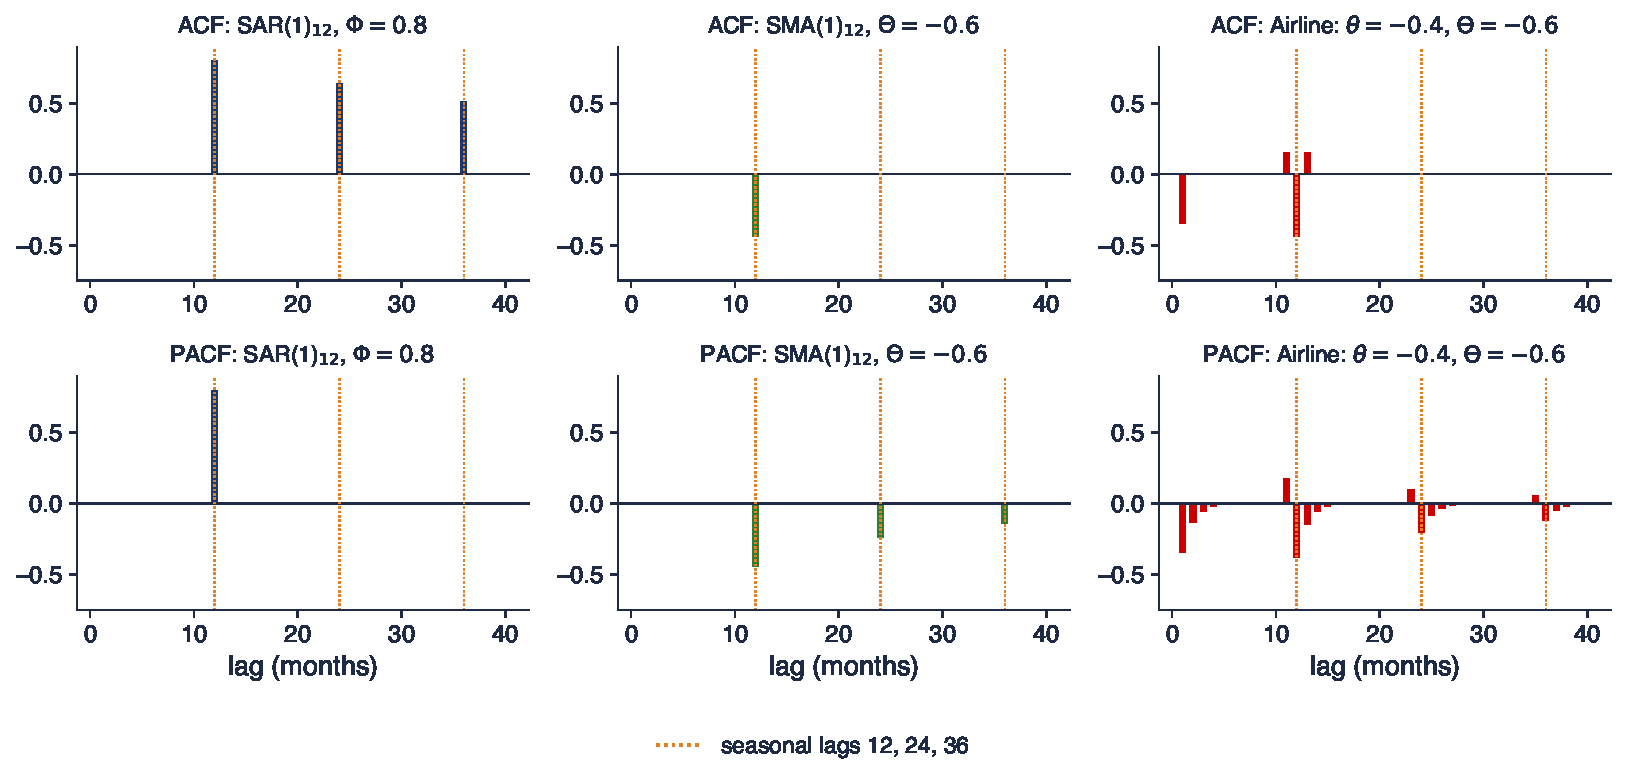
\includegraphics[width=0.97\textwidth,height=0.66\textheight,keepaspectratio]{tsa_ch4_theory_acf.pdf}
\end{center}
\vspace{-0.25cm}
\begin{itemize}
    \item Lunar, $s = 12$; panoul airline arată partea staționară $w_t = \Delta\Delta_{12}y_t$
\end{itemize}
\quantlet{TSA\_ch4\_sarima\_theory}{\qlurl{TSA_ch4_sarima_theory}}
\end{frame}

\begin{frame}{Interpretarea tiparelor sezoniere}
\itemsize{\small}
\begin{itemize}
    \item AR(1) sezonier: ACF descrește geometric la lagurile 12, 24, 36 ($0{,}8$; $0{,}64$; $0{,}512$); PACF are o singură valoare nenulă la lagul 12
    \begin{itemize}
        \item regula AR din \tsachlink{https://danpele.github.io/Time-Series-Analysis/RO/Cursuri/capitol2_modele_arma.pdf}{Capitolul 2}, citită doar la multiplii lui $s$
    \end{itemize}
    \item MA(1) sezonier: ACF se anulează după lagul 12; PACF descrește la 12, 24, 36 (\ensuremath{-}0{,}242 la lagul 24)
    \item Airline: valori nenule la 1 (\ensuremath{-}0{,}345) și 12 (\ensuremath{-}0{,}441), cu „sateliți” la 11 și 13 (0{,}152)
    \begin{itemize}
        \item sateliții sînt produsul $\rho_1\rho_{12}$: amprenta structurii multiplicative
    \end{itemize}
\end{itemize}
\end{frame}

\begin{frame}{Identificarea modelelor SARIMA}
\itemsize{\footnotesize}
\begin{center}
\footnotesize
\begin{tabular}{lll}
\toprule
\textbf{După diferențiere} & \textbf{ACF} & \textbf{PACF} \\
\midrule
AR($P$) sezonier & descrește la $s, 2s, \dots$ & se anulează după lagul $Ps$ \\
MA($Q$) sezonier & se anulează după lagul $Qs$ & descrește la $s, 2s, \dots$ \\
partea obișnuită & lagurile $1, 2, \dots$ ca în \tsachlink{https://danpele.github.io/Time-Series-Analysis/RO/Cursuri/capitol2_modele_arma.pdf}{Capitolul 2} & lagurile $1, 2, \dots$ ca în \tsachlink{https://danpele.github.io/Time-Series-Analysis/RO/Cursuri/capitol2_modele_arma.pdf}{Capitolul 2} \\
produsul celor două & sateliți la $ks \pm j$ & sateliți la $ks \pm j$ \\
\bottomrule
\end{tabular}
\end{center}
\begin{itemize}
    \item \textbf{Pașii}
    \begin{itemize}
        \item 1. Stabilizați varianța (logaritmi sau Box--Cox, \refBoxCox); 2. alegeți $D$ (graficul sezonier, HEGY, OCSB), apoi $d$ (\tsachlink{https://danpele.github.io/Time-Series-Analysis/RO/Cursuri/capitol3_radacini_unitare_modele_arima.pdf}{Capitolul 3})
        \item 3. Citiți $P, Q$ la lagurile sezoniere și $p, q$ la primele laguri; 4. păstrați ordinele mici: $P, Q \le 1$ sînt aproape întotdeauna suficiente
    \end{itemize}
\end{itemize}
\end{frame}

\begin{frame}{Estimarea și alegerea modelului}
\itemsize{\small}
\begin{itemize}
    \item \textbf{Verosimilitatea maximă} pentru seria diferențiată (forma în spațiul stărilor, \texttt{SARIMAX} din \texttt{statsmodels})
    \begin{itemize}
        \item se pierd $s + 1$ observații prin $\Delta\Delta_s$; constanta lipsește cînd $d + D \ge 2$ (ar însemna un trend pătratic)
    \end{itemize}
    \item \textbf{Criteriile informaționale}: AICc $=$ AIC $+ \frac{2k(k + 1)}{n - k - 1}$ și BIC, comparate \textbf{doar} între modele cu aceleași $d$ și $D$
    \begin{itemize}
        \item $k$: numărul parametrilor estimați; $n$: numărul de observații după diferențiere
        \item diferențierea schimbă datele pe care se calculează verosimilitatea
    \end{itemize}
    \item \textbf{SARIMA automat}: o căutare pas cu pas după $(p, q, P, Q)$ cu AICc, după alegerea lui $d$ și $D$ prin teste (\refHK)
    \begin{itemize}
        \item în Python: \texttt{pmdarima.auto\_arima(y, m=12)}; verificați întotdeauna reziduurile și comparați cu un reper
    \end{itemize}
    \item \textbf{Diagnosticarea}: Ljung--Box cu laguri dincolo de $s$ (de exemplu $m = 2s$) și $m - p - q - P - Q$ grade de libertate (\refLB)
\end{itemize}
\end{frame}

\begin{frame}{Prognoza cu modele SARIMA}
\itemsize{\small}
\begin{itemize}
    \item Ca pentru ARIMA (\tsachlink{https://danpele.github.io/Time-Series-Analysis/RO/Cursuri/capitol3_radacini_unitare_modele_arima.pdf}{Capitolul 3}): scriem modelul ca ecuație pentru $y_t$; înlocuim șocurile viitoare cu 0, valorile viitoare cu prognozele lor și șocurile trecute cu reziduuri
    \begin{itemize}
        \item airline: $\hat y_{T+h} = \hat y_{T+h-1} + \hat y_{T+h-s} - \hat y_{T+h-s-1} + (\text{termeni MA cît timp } h \le s + 1)$
    \end{itemize}
    \item \textbf{Funcția de prognoză pe termen lung} a modelului airline: un tipar sezonier fix pe o dreaptă
    \begin{itemize}
        \item tiparul este o medie ponderată exponențial a tiparelor trecute, cu ponderea $1 + \Theta$ pentru anul cel mai recent
        \item $\Theta \to -1$: un tipar fix (determinist); $\Theta = 0$: tiparul de anul trecut repetat (sezonier naiv)
    \end{itemize}
    \item Intervalele se lărgesc cu $h$ (două rădăcini unitare); pentru $\ln y$, $\exp(\hat y_{T+h})$ este \textbf{mediana} prognozei
    \begin{itemize}
        \item media este $\exp(\hat y_{T+h} + \sigma_h^2/2)$, puțin mai mare; $\sigma_h^2$: varianța erorii de prognoză la orizontul $h$
    \end{itemize}
\end{itemize}
\end{frame}

\begin{frame}{Exemplu rezolvat: prognoza unui MA sezonier}
\itemsize{\small}
\begin{itemize}
    \item SARIMA$(0,0,0)(0,1,1)_4$ trimestrial: $y_t = y_{t-4} + \varepsilon_t + \Theta\varepsilon_{t-4}$, $\Theta = -0{,}6$
    \begin{itemize}
        \item ultimul an: $y_{T-3}, \dots, y_T = 100; 120; 130; 140$; reziduurile $\hat\varepsilon_{T-3}, \dots, \hat\varepsilon_T = 2; -1; 0; 3$
    \end{itemize}
    \item $\hat y_{T+1} = y_{T-3} + \Theta\hat\varepsilon_{T-3} = 100 - 0{,}6 \cdot 2 = 98{,}8$
    \begin{itemize}
        \item $\hat y_{T+2} = 120{,}6$, $\hat y_{T+3} = 130{,}0$, $\hat y_{T+4} = 138{,}2$
    \end{itemize}
    \item $\hat y_{T+5} = \hat y_{T+1} = 98{,}8$: după un an, termenul MA dispare și tiparul prognozei se repetă
    \begin{itemize}
        \item o surpriză pozitivă mare în ultimul sezon ($\hat\varepsilon_T = 3$) scade prognoza pentru acel sezon cu $0{,}6 \cdot 3$: o corecție parțială
    \end{itemize}
\end{itemize}
\end{frame}

\begin{frame}{Recapitulare: modele SARIMA}
\itemsize{\small}
\begin{itemize}
    \item SARIMA înmulțește polinoame obișnuite și sezoniere: $\phi(L)\Phi(L^s)\Delta^d\Delta_s^Dy_t = \theta(L)\Theta(L^s)\varepsilon_t$
    \item Identificarea: regulile din \tsachlink{https://danpele.github.io/Time-Series-Analysis/RO/Cursuri/capitol2_modele_arma.pdf}{Capitolul 2} la lagurile $s, 2s, \dots$, plus sateliții de la $ks \pm j$
    \item Comparați AICc doar pentru aceleași $d$ și $D$; verificați Ljung--Box dincolo de lagul $s$
    \item Prognoza airline: un tipar sezonier pe o dreaptă, actualizat cu ponderea $1 + \Theta$
\end{itemize}
\end{frame}


%=============================================================================
\section{Studiu de caz: modelul airline}
%=============================================================================

\begin{frame}{Box, Jenkins și pasagerii companiilor aeriene}
\itemsize{\footnotesize}
\begin{columns}[T]
\begin{column}{0.56\textwidth}
\begin{itemize}
    \item \refBJ{} (prima ediție în 1970) au modelat totalurile lunare ale pasagerilor internaționali, 1949--1960 (144 de luni)
    \begin{itemize}
        \item creștere plus un vîrf de vară a cărui mărime crește cu nivelul
        \item modelul lor, SARIMA$(0,1,1)(0,1,1)_{12}$ pentru $\ln y_t$, poartă de atunci numele de „model airline”
    \end{itemize}
    \item Motivele longevității modelului
    \begin{itemize}
        \item doi parametri se potrivesc multor serii sezoniere: comerț, producție, vînzări cu amănuntul, energie
        \item este modelul de referință al etapei regARIMA din programele de ajustare sezonieră (secțiunea 6)
    \end{itemize}
\end{itemize}
\end{column}
\begin{column}{0.40\textwidth}
\centering
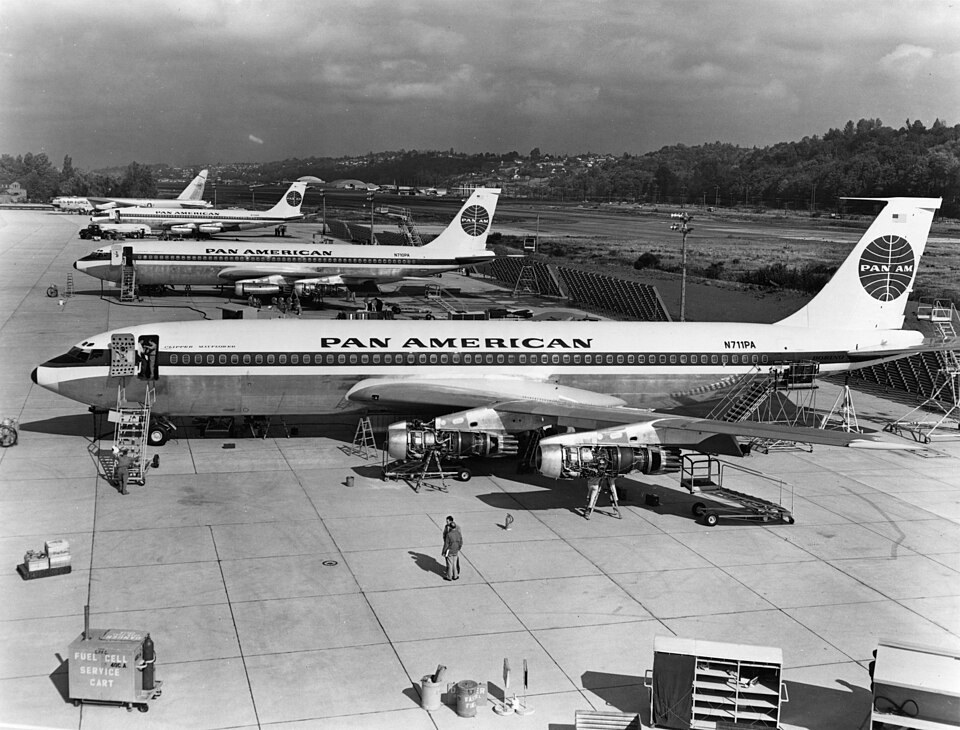
\includegraphics[height=0.36\textheight]{ch4_pan_am_707_1958.jpg}\\[1mm]
\imgcap{Primele avioane Boeing 707 pentru Pan American, Seattle, 1958}
\imgcredit{https://commons.wikimedia.org/wiki/File:Three_Pan_Am_Boeing_707_awaiting_delivery.jpg}{Foto: autor necunoscut (1958); domeniu public; Wikimedia Commons}
\end{column}
\end{columns}
\end{frame}

\begin{frame}{Identificarea modelului airline}
\itemsize{\footnotesize}
\begin{center}
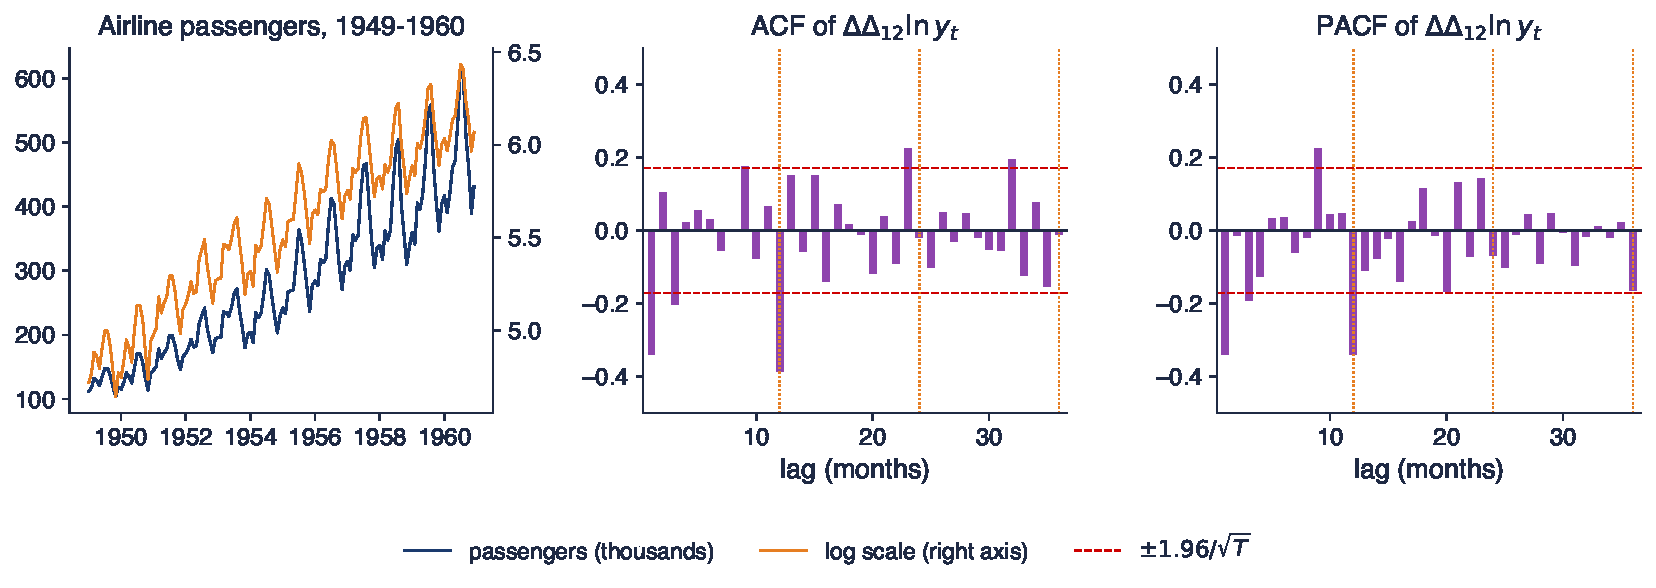
\includegraphics[width=0.97\textwidth,height=0.58\textheight,keepaspectratio]{tsa_ch4_airline.pdf}
\end{center}
\vspace{-0.25cm}
\begin{itemize}
    \item Stînga: pasagerii și logaritmul lor; mijloc și dreapta: ACF și PACF pentru $w_t = \Delta\Delta_{12}\ln y_t$, 131 de observații
\end{itemize}
\quantlet{TSA\_ch4\_airline}{\qlurl{TSA_ch4_airline}}
\end{frame}

\begin{frame}{Interpretarea corelogramelor airline}
\itemsize{\small}
\begin{itemize}
    \item Logaritmul face constantă amplitudinea verii: tiparul multiplicativ devine aditiv
    \item ACF pentru $w_t$: $\ensuremath{-}0{,}34$ la lagul 1 și $\ensuremath{-}0{,}39$ la lagul 12, în afara benzii $\pm 0{,}17$
    \begin{itemize}
        \item un MA(1) obișnuit și un MA(1) sezonier; lagul 3 ($\ensuremath{-}0{,}20$) este la limită
    \end{itemize}
    \item PACF descrește la lagurile 1, 2, 3 și 12, 24: în acord cu termeni MA, nu cu termeni AR
    \item Concluzia: SARIMA$(0,1,1)(0,1,1)_{12}$, exact modelul lui Box și Jenkins
\end{itemize}
\end{frame}

\begin{frame}{Modelul airline: prognoze în afara eșantionului}
\itemsize{\footnotesize}
\begin{center}
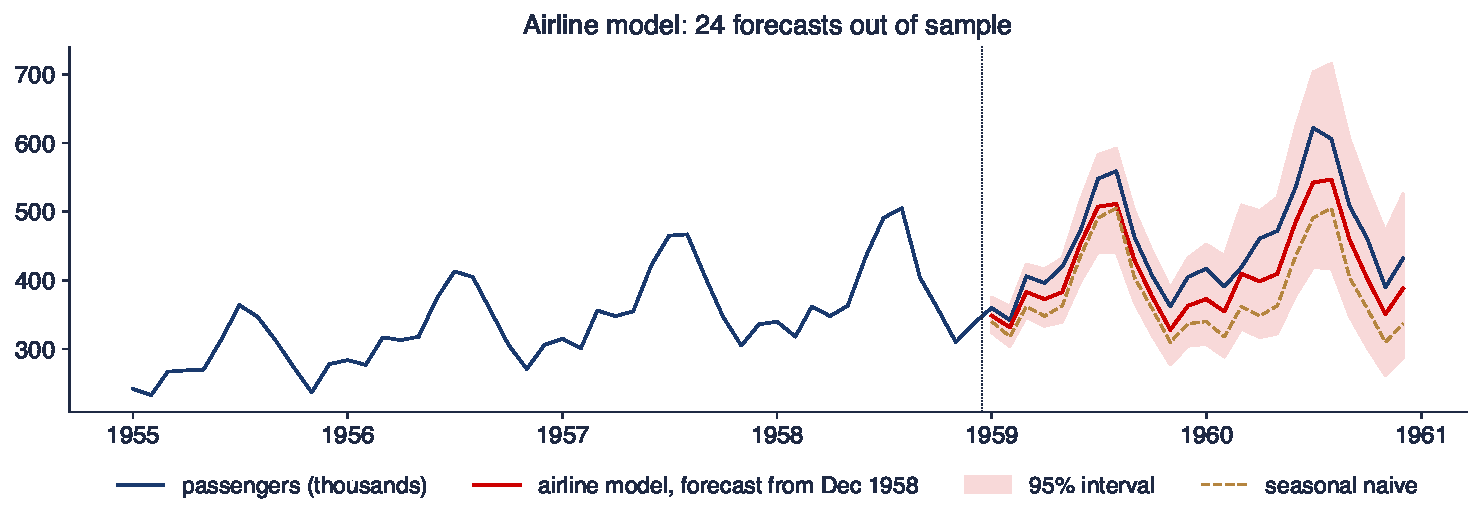
\includegraphics[width=0.97\textwidth,height=0.56\textheight,keepaspectratio]{tsa_ch4_airline_fc.pdf}
\end{center}
\vspace{-0.25cm}
\begin{itemize}
    \item Estimat pe 1949--1958, prognoze pentru cele 24 de luni din 1959--1960, transformate înapoi din $\ln y$
\end{itemize}
\quantlet{TSA\_ch4\_airline}{\qlurl{TSA_ch4_airline}}
\end{frame}

\begin{frame}{Interpretarea prognozelor airline}
\itemsize{\footnotesize}
\begin{itemize}
    \item 1949--1958: $\hat\theta = \ensuremath{-}0{,}342$ (0{,}087), $\hat\Theta = \ensuremath{-}0{,}541$ (0{,}105); întregul eșantion: $\hat\theta = \ensuremath{-}0{,}402$ (0{,}073), $\hat\Theta = \ensuremath{-}0{,}557$ (0{,}096)
    \begin{itemize}
        \item abaterea standard a reziduurilor 3{,}7\% pe lună; Ljung--Box $Q^*(24)$ cu 22 de grade de libertate, p = 0{,}37
    \end{itemize}
    \item MAPE pe 1959--1960: 8{,}5\% pentru modelul airline, 15{,}5\% pentru prognoza sezonieră naivă (care ignoră creșterea)
    \item Decembrie 1960: prognoza 388, intervalul [286; 526], valoarea reală 432: în interior, dar modelul subestimează creșterea din 1959--1960
    \begin{itemize}
        \item lățimea intervalului crește de la 51 (prima lună) la 239 (luna 24): două rădăcini unitare
    \end{itemize}
\end{itemize}
\end{frame}


%=============================================================================
\section{Studiu de caz: PIB-ul neajustat al României}
%=============================================================================

\begin{frame}{Modele SARIMA pentru PIB-ul României}
\itemsize{\footnotesize}
\begin{center}
\scriptsize
\begin{tabular}{lrrrr}
\toprule
\textbf{Modelul} & \textbf{AICc} & \textbf{BIC} & \textbf{LB(8), p} & $\hat\sigma$ (\%) \\
\midrule
$(0,1,1)(0,1,1)_4$ & 520{,}1 & 527{,}6 & 0{,}157 & 3{,}05 \\
$(0,1,0)(0,1,1)_4$ & 519{,}7 & \textbf{524{,}8} & 0{,}286 & 3{,}08 \\
$(1,1,0)(0,1,1)_4$ & 520{,}7 & 528{,}3 & 0{,}156 & 3{,}06 \\
$(1,1,1)(0,1,1)_4$ & \textbf{518{,}3} & 528{,}4 & 0{,}467 & 2{,}98 \\
$(0,1,2)(0,1,1)_4$ & 518{,}8 & 528{,}8 & 0{,}575 & 3{,}00 \\
$(0,1,1)(1,1,0)_4$ & 529{,}9 & 537{,}5 & 0{,}003 & 3{,}22 \\
$(0,1,1)(1,1,1)_4$ & 522{,}2 & 532{,}2 & 0{,}118 & 3{,}05 \\
$(0,1,1)(0,1,0)_4$ & 545{,}1 & 550{,}2 & 0{,}005 & 3{,}52 \\
\bottomrule
\end{tabular}
\end{center}
\begin{itemize}
    \item $y_t = 100\ln Y_t$, PIB real neajustat, T1 2000--T2 2026, $T = 106$; verosimilitate maximă; toate cu $d = D = 1$, deci criteriile sînt comparabile
    \item Ljung--Box pe 8 laguri, cu $8 - p - q - P - Q$ grade de libertate
\end{itemize}
\end{frame}

\begin{frame}{Interpretarea tabelului de modele}
\itemsize{\small}
\begin{itemize}
    \item BIC alege $(0,1,0)(0,1,1)_4$: doar termenul MA sezonier; AICc alege $(1,1,1)(0,1,1)_4$
    \begin{itemize}
        \item modelul AICc are $\hat\phi = 0{,}78$ și $\hat\theta = \ensuremath{-}0{,}94$: aproape un factor comun (\tsachlink{https://danpele.github.io/Time-Series-Analysis/RO/Cursuri/capitol2_modele_arma.pdf}{Capitolul 2}), cu un cîștig mic
        \item modelul airline: $\hat\theta = \ensuremath{-}0{,}171$ (0{,}109), nesemnificativ; $\hat\Theta = \ensuremath{-}0{,}585$
    \end{itemize}
    \item Un AR sezonier în locul MA sezonier sau niciun termen sezonier: criterii mult mai slabe și reziduuri corelate
    \item Păstrăm modelul BIC: un singur parametru, $\hat\Theta = \ensuremath{-}0{,}577$ (0{,}075), $\hat\sigma = 3{,}08\%$
\end{itemize}
\end{frame}

\begin{frame}{Diagnosticarea modelului pentru PIB}
\itemsize{\footnotesize}
\begin{center}
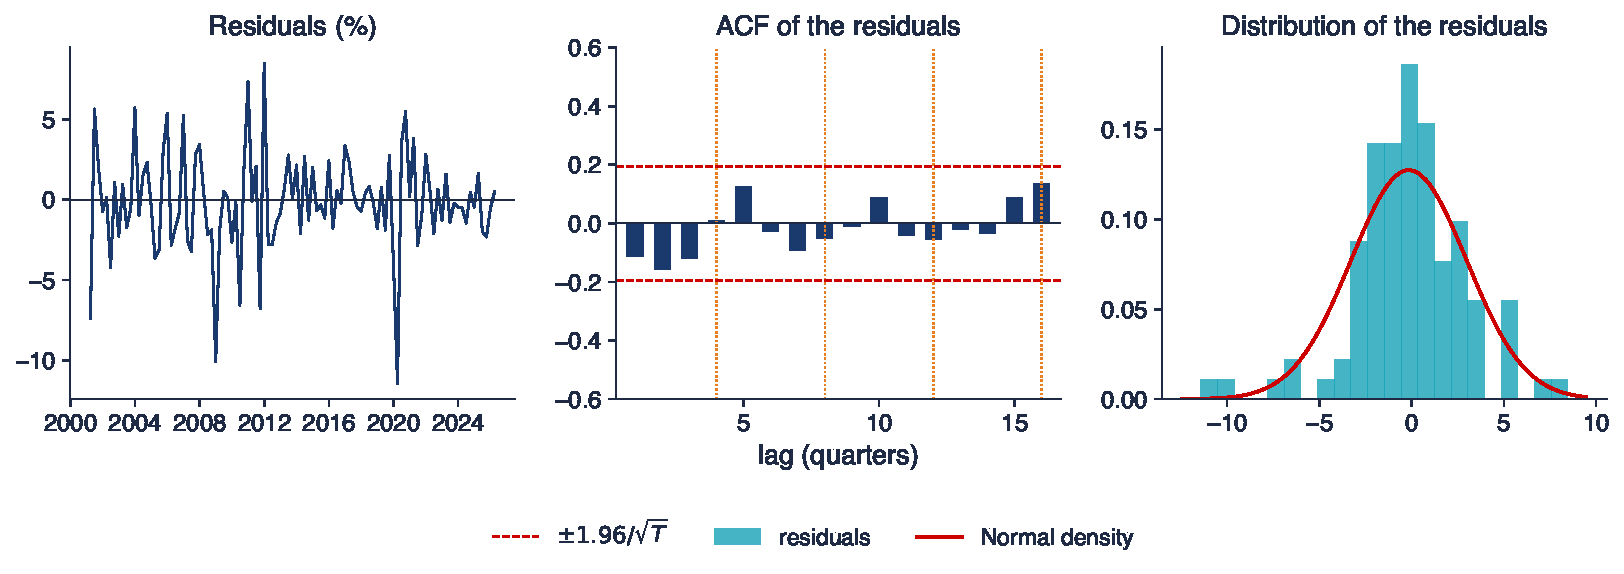
\includegraphics[width=0.97\textwidth,height=0.56\textheight,keepaspectratio]{tsa_ch4_gdp_diag.pdf}
\end{center}
\vspace{-0.25cm}
\begin{itemize}
    \item SARIMA$(0,1,0)(0,1,1)_4$ pentru $100\ln Y_t$: reziduurile, ACF a lor și distribuția lor
\end{itemize}
\quantlet{TSA\_ch4\_gdp\_case}{\qlurl{TSA_ch4_gdp_case}}
\end{frame}

\begin{frame}{Interpretarea diagnosticării PIB}
\itemsize{\small}
\begin{itemize}
    \item Nu rămîne autocorelație: $Q^*(8) = 8{,}55$ cu 7 grade de libertate, p = 0{,}286; $Q^*(12)$: p = 0{,}526
    \begin{itemize}
        \item nicio valoare semnificativă la lagurile sezoniere 4, 8, 12, 16: structura sezonieră este surprinsă
    \end{itemize}
    \item Nu este distribuția Normală: Jarque--Bera 22{,}0 (p $<$\,0{,}001); cel mai mare reziduu este \ensuremath{-}11{,}4\% în T2 2020 ($\ensuremath{-}3{,}6$ abateri standard): perioada de lockdown
    \begin{itemize}
        \item fără 2020, Jarque--Bera scade la 13{,}4: o variabilă dummy pentru valoarea aberantă ar fi pasul următor
    \end{itemize}
\end{itemize}
\end{frame}

\begin{frame}{Prognozele PIB-ului României}
\itemsize{\footnotesize}
\begin{center}
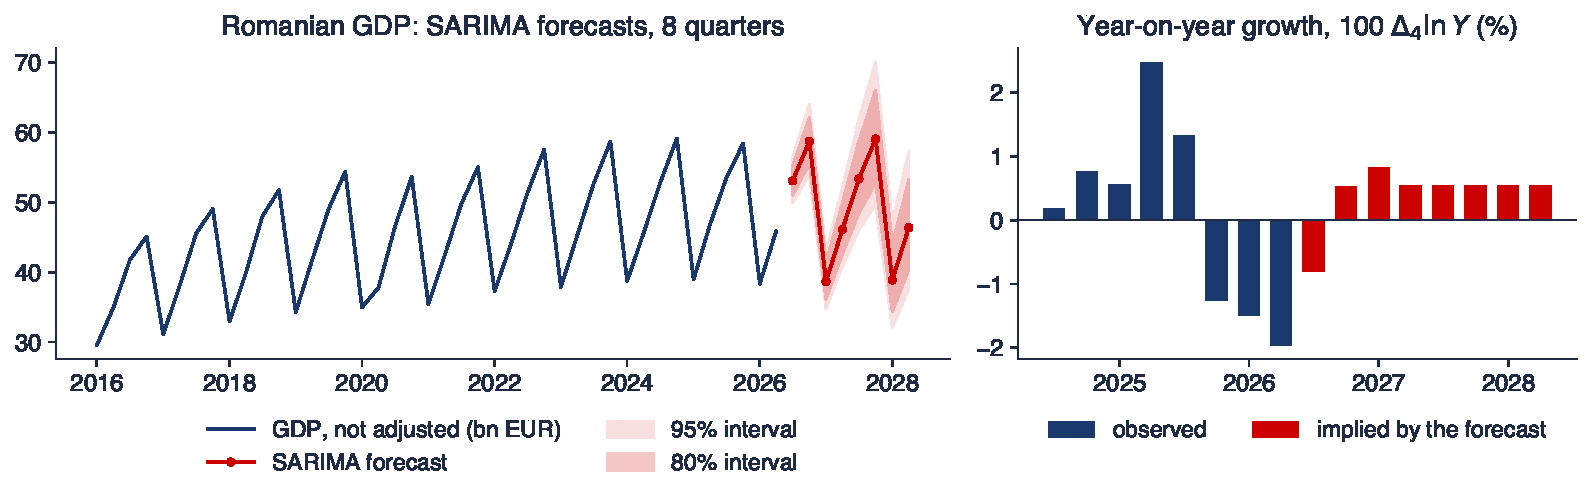
\includegraphics[width=0.97\textwidth,height=0.56\textheight,keepaspectratio]{tsa_ch4_gdp_fc.pdf}
\end{center}
\vspace{-0.25cm}
\begin{itemize}
    \item SARIMA$(0,1,0)(0,1,1)_4$, 8 trimestre, din T3 2026 pînă în T2 2028, intervale de 80\% și 95\%; dreapta: creșterea anuală implicată
\end{itemize}
\quantlet{TSA\_ch4\_gdp\_case}{\qlurl{TSA_ch4_gdp_case}}
\end{frame}

\begin{frame}{Interpretarea prognozelor PIB}
\itemsize{\small}
\begin{itemize}
    \item Ultima valoare: 45{,}9 mld. EUR în T2 2026; prognozele 53{,}1; 58{,}7; 38{,}7; 46{,}1 mld. EUR pentru următoarele patru trimestre
    \begin{itemize}
        \item intervalul de 95\% pentru primul trimestru [50{,}0; 56{,}4], pentru al optulea [37{,}6; 57{,}2]
    \end{itemize}
    \item Creșterea anuală implicată: \ensuremath{-}0{,}81\%; 0{,}53\%; 0{,}83\%; 0{,}55\%, apoi constant 0{,}55\%
    \begin{itemize}
        \item modelul extrapolează creșterea slabă recentă; nu conține informații despre politica fiscală sau fondurile europene
    \end{itemize}
    \item Tiparul sezonier al prognozei este o medie ponderată a anilor trecuți, cu ponderea $1 + \hat\Theta = 0{,}42$ pentru anul cel mai recent
\end{itemize}
\end{frame}

\begin{frame}{Recapitulare: pasagerii aerieni și PIB-ul României}
\itemsize{\small}
\begin{itemize}
    \item Logaritmi, apoi $\Delta\Delta_s$, apoi termeni MA la lagurile 1 și $s$: rețeta airline funcționează pentru ambele serii
    \item Pentru PIB, BIC renunță la termenul MA obișnuit; AICc alege un ARMA(1,1) aproape redundant
    \item Reziduurile sînt curate, cu excepția valorii aberante din 2020
    \item Prognozele repetă un tipar sezonier netezit pe o linie de trend, cu intervale tot mai largi
\end{itemize}
\end{frame}


%=============================================================================
\section{Ajustarea sezonieră în practică}
%=============================================================================

\begin{frame}{Rostul ajustării sezoniere în statistica oficială}
\itemsize{\small}
\begin{itemize}
    \item Utilizatorii vor să știe dacă economia \textbf{a crescut în acest trimestru}, nu dacă T3 este mai mare decît T2
    \begin{itemize}
        \item T1 2026: PIB-ul neajustat s-a modificat cu \ensuremath{-}42{,}1\% (puncte logaritmice) față de trimestrul anterior; seria ajustată cu \ensuremath{-}0{,}06\%
        \item prima cifră este doar sezon; doar a doua spune ceva despre ciclul economic
    \end{itemize}
    \item \textbf{Ajustarea sezonieră}: estimăm componentele sezonieră și de calendar și le eliminăm: $y_t^{SA} = y_t - \hat S_t - \hat C_t$ (sau $y_t/(\hat S_t\hat C_t)$)
    \begin{itemize}
        \item descompunerea clasică și STL din \tsachlink{https://danpele.github.io/Time-Series-Analysis/RO/Cursuri/capitol0_introducere.pdf}{Capitolul 0} sînt variante simple ale acestei idei
    \end{itemize}
    \item Pentru prognoza cu SARIMA folosim seria \textbf{neajustată}: filtrele de ajustare schimbă autocorelațiile și sînt revizuite cînd apar date noi
\end{itemize}
\end{frame}

\begin{frame}{X-11 și X-13ARIMA-SEATS}
\itemsize{\footnotesize}
\begin{columns}[T]
\begin{column}{0.66\textwidth}
\begin{itemize}
    \item \textbf{X-11} (US Census Bureau, anii 1960; \refLadiray): medii mobile aplicate iterativ
    \begin{itemize}
        \item o medie mobilă centrată $2 \times 12$ pentru trend, apoi medii mobile $3 \times 3$ și $3 \times 5$ ale fiecărei luni de-a lungul anilor pentru factorii sezonieri
    \end{itemize}
    \item \textbf{X-12-ARIMA} (\refFindley) și \textbf{X-13ARIMA-SEATS} adaugă o \textbf{preajustare regARIMA}:
    \begin{itemize}
        \item regresie cu erori SARIMA (adesea modelul airline) pentru valori aberante, zile lucrătoare, Paște
        \item prognozele ARIMA prelungesc seria, astfel încît filtrele simetrice funcționează și la capăt: revizuiri mai mici
        \item apoi filtrele X-11 sau SEATS (descompunerea pe baza modelului ARIMA)
    \end{itemize}
    \item UE: Eurostat și institutele naționale urmează \refESS, cu programul JDemetra+ (X-13 și TRAMO-SEATS)
\end{itemize}
\end{column}
\begin{column}{0.30\textwidth}
\centering
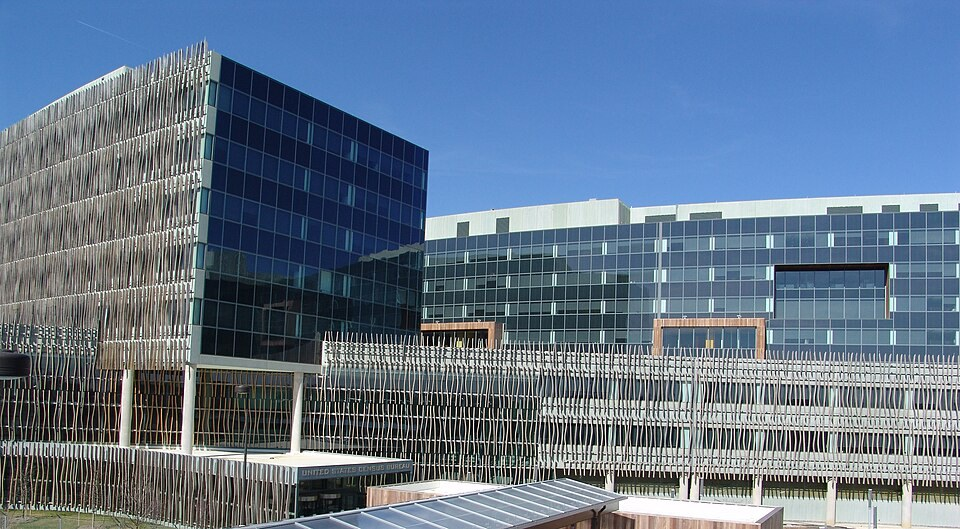
\includegraphics[height=0.24\textheight]{ch4_census_bureau_2007.jpg}\\[1mm]
\imgcap{US Census Bureau, Suitland, Maryland: locul de naștere al X-11 și X-13}
\imgcredit{https://commons.wikimedia.org/wiki/File:Census_Bureau_headquarters,_Suitland,_Maryland,_2007.jpg}{Foto: United States Census Bureau (2007); domeniu public; Wikimedia Commons}
\end{column}
\end{columns}
\end{frame}

\begin{frame}{Seriile Eurostat: NSA, CA, SA, SCA}
\itemsize{\small}
\begin{itemize}
    \item Fiecare serie apare în mai multe variante (dimensiunea \texttt{s\_adj}):
    \begin{itemize}
        \item \textbf{NSA}: neajustată sezonier (datele brute)
        \item \textbf{CA}: ajustată doar pentru efectele de calendar (zile lucrătoare, sărbători)
        \item \textbf{SA}: ajustată sezonier; \textbf{SCA}: ajustată sezonier și pentru efectele de calendar
    \end{itemize}
    \item Varianta potrivită pentru fiecare întrebare
    \begin{itemize}
        \item creșterea față de trimestrul sau luna anterioară: SCA
        \item creșterea față de anul anterior: NSA sau CA (tiparul sezonier se anulează, calendarul nu)
        \item modelarea și prognoza SARIMA: NSA, cu regresori de calendar
    \end{itemize}
    \item Totalurile anuale NSA și SCA sînt apropiate (2024: 196{,}4 și 196{,}4 mld. EUR): ajustarea mută producția între trimestre, nu o creează
\end{itemize}
\end{frame}

\begin{frame}{Serii neajustate și ajustate}
\itemsize{\footnotesize}
\begin{center}
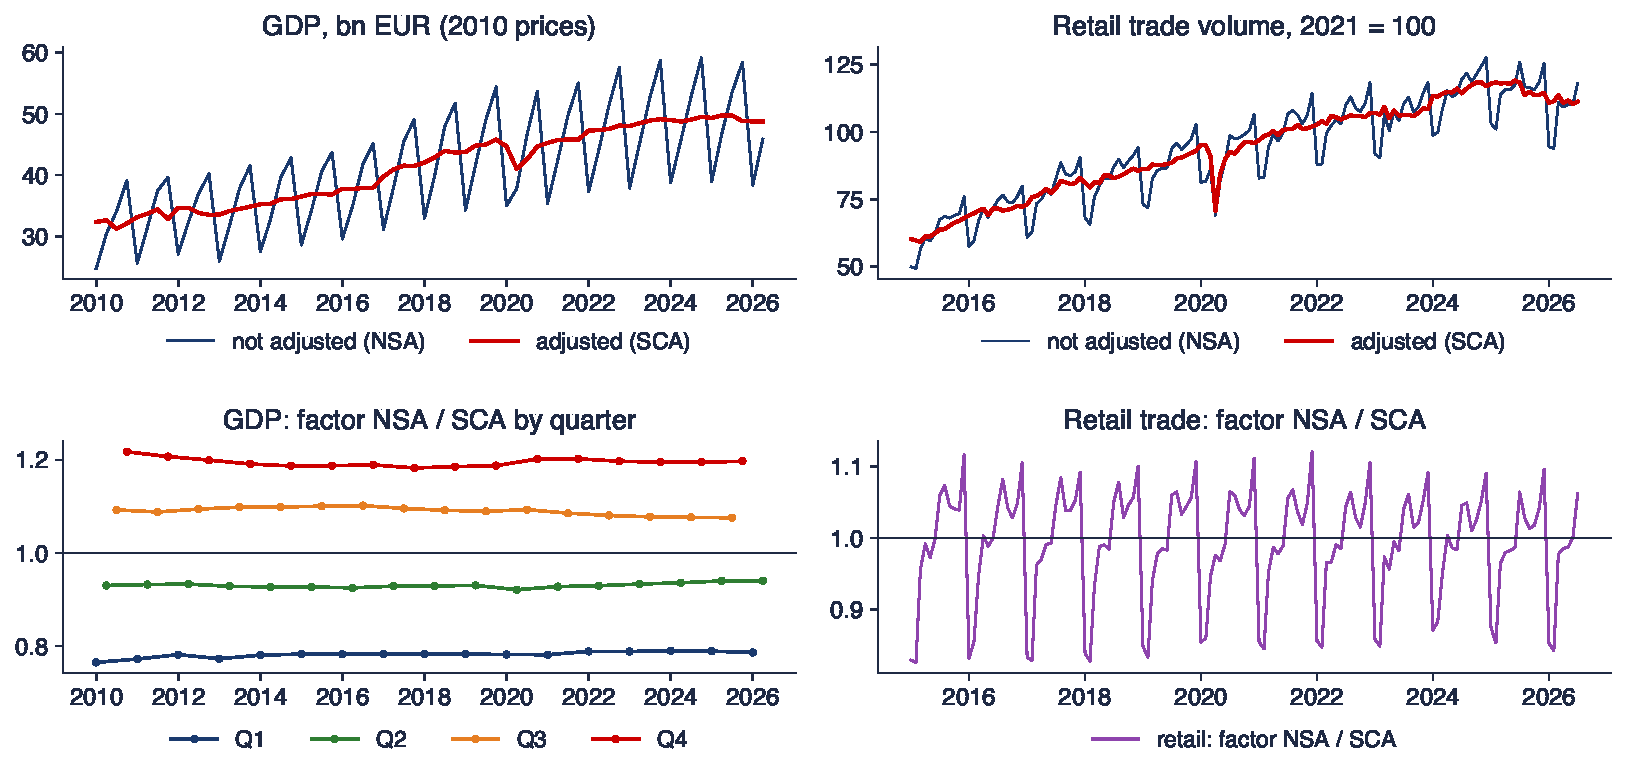
\includegraphics[width=0.97\textwidth,height=0.66\textheight,keepaspectratio]{tsa_ch4_sa_nsa.pdf}
\end{center}
\vspace{-0.25cm}
\begin{itemize}
    \item Eurostat NSA și SCA: PIB (stînga sus) și comerțul cu amănuntul (dreapta sus); jos: factorii sezonieri și de calendar implicați, NSA/SCA
\end{itemize}
\quantlet{TSA\_ch4\_seasonal\_data}{\qlurl{TSA_ch4_seasonal_data}}
\end{frame}

\begin{frame}{Interpretarea seriilor ajustate}
\itemsize{\footnotesize}
\begin{itemize}
    \item Factorii PIB 2015--2019: T1 0{,}78, T2 0{,}93, T3 1{,}10, T4 1{,}19: producția din T1 este cu aproximativ o cincime sub un trimestru mediu
    \begin{itemize}
        \item factorii se mișcă lent de-a lungul anilor: sezonalitatea stochastică măsurată de $\hat\Theta$
    \end{itemize}
    \item Comerțul cu amănuntul: factorul pentru decembrie 1{,}10, pentru ianuarie 0{,}84 (2016--2019): cumpărăturile de Crăciun, apoi minimul din ianuarie
    \item Factorul pentru comerț sare și de la o lună la alta din cauza zilelor lucrătoare și a Paștelui: partea de calendar a SCA (secțiunea 7)
    \item PIB-ul ajustat arată scăderea din 2020 și stagnarea din 2025--2026 pe care seria brută le ascunde
\end{itemize}
\end{frame}

\begin{frame}{Recapitulare: ajustarea sezonieră}
\itemsize{\small}
\begin{itemize}
    \item Ajustarea sezonieră elimină $\hat S_t$ și $\hat C_t$ pentru a arăta trendul și ciclul
    \item X-13ARIMA-SEATS: preajustare regARIMA (valori aberante, calendar, prognoze), apoi X-11 sau SEATS; în UE, JDemetra+
    \item Creșterea față de trimestrul anterior: SCA; creșterea anuală: NSA sau CA; prognoza SARIMA: NSA
\end{itemize}
\end{frame}


%=============================================================================
\section{Termeni Fourier și efecte de calendar}
%=============================================================================

\begin{frame}{Variabile dummy sezoniere și termeni Fourier}
\itemsize{\small}
\begin{itemize}
    \item \textbf{Variabile dummy}: $y_t = \beta_0 + \sum_{j=2}^{s}\gamma_jD_{jt} + u_t$: $s - 1$ coeficienți, orice formă
    \begin{itemize}
        \item $\beta_0$: nivelul sezonului 1; $\gamma_j$: diferența dintre sezonul $j$ și sezonul 1
        \item prea mulți pentru $s = 52$ de săptămîni, $s = 168$ ore sau $s = 365$ de zile; imposibil pentru $s = 365{,}25$
    \end{itemize}
    \item \textbf{Termeni Fourier} pentru o perioadă $m$: $\sum_{k=1}^{K}\left[\alpha_k\sin\frac{2\pi kt}{m} + \beta_k\cos\frac{2\pi kt}{m}\right]$
    \begin{itemize}
        \item $\alpha_k, \beta_k$: coeficienții armonicei $k$, o undă cu $k$ cicluri pe perioadă; $K$: numărul de perechi sinus--cosinus
        \item $2K$ coeficienți; $K = m/2$ reproduce exact variabilele dummy (pentru $m$ par); un $K$ mic dă un tipar neted
        \item $m$ poate fi neîntreg și se pot combina mai multe perioade: de exemplu $K = 5$ pentru $m = 24$ și $K = 4$ pentru $m = 168$ dau 18 regresori în locul a $23 + 167$
    \end{itemize}
    \item $K$ se alege cu AICc sau prin validare încrucișată; aceiași termeni se află în TBATS și Prophet (secțiunea 9)
\end{itemize}
\end{frame}

\begin{frame}{Aproximarea Fourier a unui tipar sezonier}
\itemsize{\footnotesize}
\begin{center}
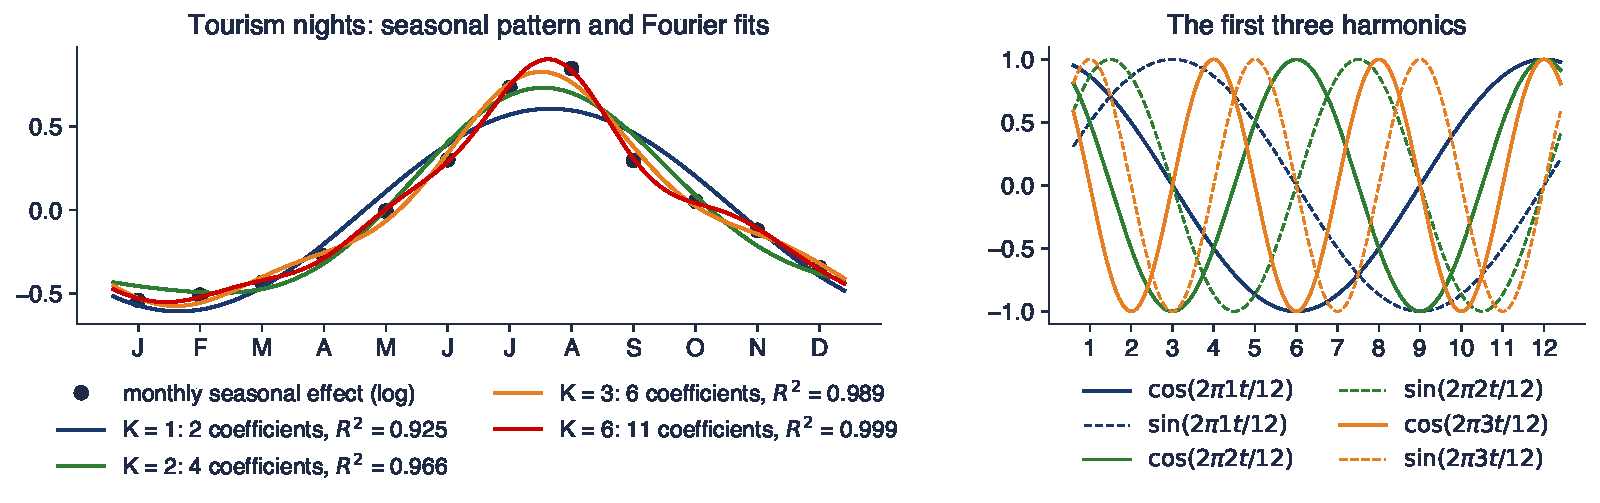
\includegraphics[width=0.97\textwidth,height=0.58\textheight,keepaspectratio]{tsa_ch4_fourier.pdf}
\end{center}
\vspace{-0.25cm}
\begin{itemize}
    \item Efectul sezonier lunar al $\ln$(înnoptări turistice), 2012--2019, după eliminarea unei medii centrate pe 13 luni; ajustări cu $K = 1, 2, 3, 6$
\end{itemize}
\quantlet{TSA\_ch4\_calendar\_fourier}{\qlurl{TSA_ch4_calendar_fourier}}
\end{frame}

\begin{frame}{Interpretarea ajustărilor Fourier}
\itemsize{\small}
\begin{itemize}
    \item $K = 1$ (doi coeficienți) dă deja $R^2 = 0{,}925$: vîrful de vară este aproape o singură undă
    \begin{itemize}
        \item $K = 2$: 0{,}966; $K = 3$: 0{,}989 cu șase coeficienți în loc de unsprezece
    \end{itemize}
    \item $K = 6$ (11 coeficienți) trece prin cele 12 puncte lunare: la fel ca 11 variabile dummy, $R^2 = 0{,}999$
    \item Armonicele superioare adaugă detalii mai fine: vîrful din august cere $K \ge 3$
\end{itemize}
\end{frame}

\begin{frame}{Efecte de calendar și Paștele ortodox}
\itemsize{\footnotesize}
\begin{columns}[T]
\begin{column}{0.66\textwidth}
\begin{itemize}
    \item \textbf{Zilele lucrătoare}: o lună cu mai multe zile de luni pînă vineri care nu sînt sărbători produce și vinde mai mult
    \begin{itemize}
        \item cunoscute dinainte: un regresor care poate fi folosit în prognoze
    \end{itemize}
    \item \textbf{Sărbătorile mobile}: Paștele ortodox cade între 4 aprilie și 8 mai
    \begin{itemize}
        \item 5 mai 2024, 20 aprilie 2025, 12 aprilie 2026, 2 mai 2027: cumpărăturile se mută între martie, aprilie și mai
        \item în Python: \texttt{dateutil.easter.easter(y, EASTER\_ORTHODOX)}; Rusaliile sînt cu 49 de zile mai tîrziu
    \end{itemize}
    \item \textbf{Regresorul Paște} (\texttt{easter[w]} din X-13): $E_t$ = partea din cele $w$ zile dinaintea Duminicii Paștelui care cade în luna $t$
    \begin{itemize}
        \item $w = 10$: Paștele pe 20 aprilie dă $E_{\text{aprilie}} = 1$; pe 5 mai, $E_{\text{aprilie}} = 0{,}6$ și $E_{\text{mai}} = 0{,}4$
    \end{itemize}
\end{itemize}
\end{column}
\begin{column}{0.30\textwidth}
\centering

\includegraphics[height=0.26\textheight]{ch4_romanian_easter_eggs.jpg}\\[1mm]
\imgcap{Ouă încondeiate de Paște din România}
\imgcredit{https://commons.wikimedia.org/wiki/File:Painted_Romanian_Easter_Eggs.jpg}{Foto: jackmac34 (Pixabay); CC0; Wikimedia Commons}
\end{column}
\end{columns}
\end{frame}

\begin{frame}{Regresia cu erori SARIMA}
\itemsize{\small}
\begin{itemize}
    \item $100\ln y_t = \beta_EE_t + \beta_W\,\mathrm{WD}_t + \text{variabile dummy pentru valori aberante} + u_t$, cu $u_t \sim$ SARIMA$(0,1,1)(0,1,1)_{12}$
    \begin{itemize}
        \item $E_t$: regresorul Paște; $\mathrm{WD}_t$: numărul de zile lucrătoare din luna $t$; $\beta_E$, $\beta_W$: efectele lor, în \%
        \item modelul „regARIMA” din X-13; estimat într-un singur pas prin verosimilitate maximă (\texttt{SARIMAX} cu \texttt{exog})
        \item metoda celor mai mici pătrate care ignoră erorile SARIMA ar da erori standard greșite (\tsachlink{https://danpele.github.io/Time-Series-Analysis/RO/Cursuri/capitol3_radacini_unitare_modele_arima.pdf}{Capitolul 3}, regresia falsă)
    \end{itemize}
    \item Datele: volumul comerțului cu amănuntul, Eurostat, România, neajustat, ianuarie 2010--iulie 2026: alimente (G47\_FOOD) și total (G47)
    \begin{itemize}
        \item variabile dummy pentru aprilie și mai 2020 (lockdown)
    \end{itemize}
\end{itemize}
\end{frame}

\begin{frame}{Paștele și comerțul cu amănuntul din România}
\itemsize{\footnotesize}
\begin{center}
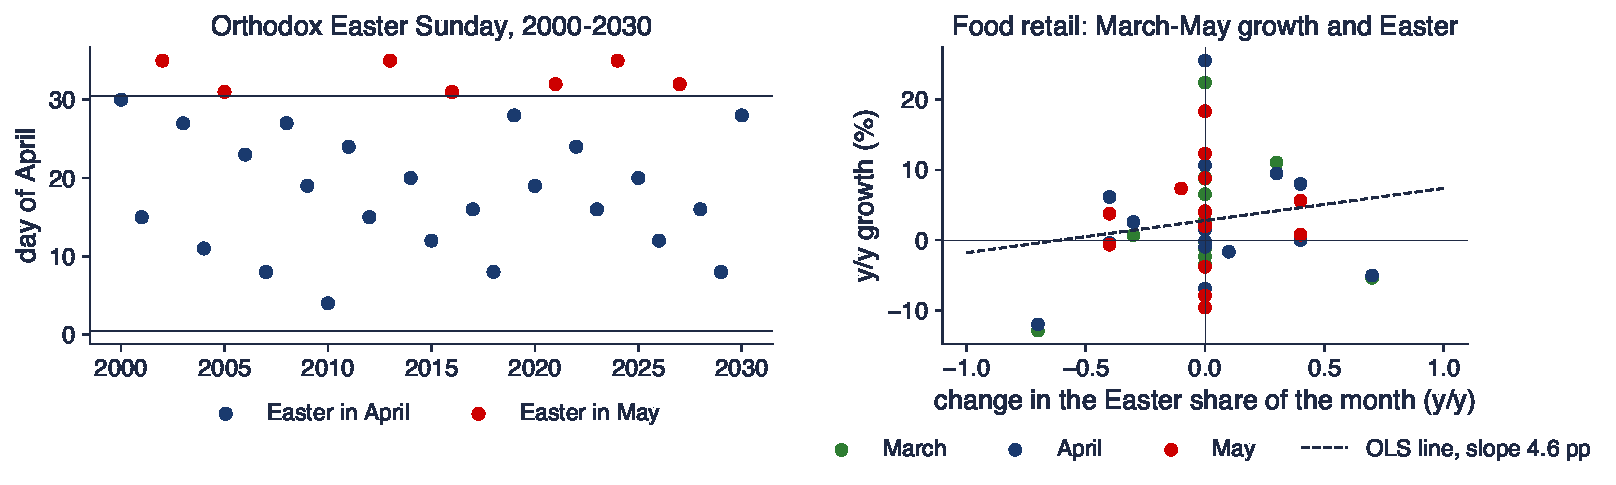
\includegraphics[width=0.97\textwidth,height=0.56\textheight,keepaspectratio]{tsa_ch4_easter.pdf}
\end{center}
\vspace{-0.25cm}
\begin{itemize}
    \item Stînga: Duminica Paștelui ortodox ca zi din aprilie (peste 30: mai); dreapta: creșterea anuală a vînzărilor de alimente în martie--mai față de modificarea ponderii Paștelui (fără 2020--2021)
\end{itemize}
\quantlet{TSA\_ch4\_calendar\_fourier}{\qlurl{TSA_ch4_calendar_fourier}}
\end{frame}

\begin{frame}{Interpretarea efectului Paștelui}
\itemsize{\footnotesize}
\begin{itemize}
    \item Alimente: $\hat\beta_E = 5{,}9\%$ (eroarea standard 2{,}3, $t = 2{,}6$): o lună care cuprinde cele 10 zile dinaintea Paștelui vinde cu aproximativ 5{,}9\% mai multe alimente
    \begin{itemize}
        \item o zi lucrătoare în plus: $+0{,}59\%$ (eroarea standard 0{,}17); aprilie 2020: $\ensuremath{-}15\%$
    \end{itemize}
    \item Totalul comerțului: Paștele $0{,}8\%$ (eroarea standard 1{,}9), nesemnificativ; zilele lucrătoare $+1{,}02\%$ (eroarea standard 0{,}15)
    \begin{itemize}
        \item efectul Paștelui se află în alimente, efectul zilelor lucrătoare în toate vînzările
    \end{itemize}
    \item Norul de puncte brut este zgomotos (panta 4{,}6 puncte procentuale): modificările TVA și prețurile mișcă și ele creșterea anuală; regresia separă efectele
    \item Paștele a căzut în mai în 2002; 2005; 2013; 2016; 2021; 2024: cine ignoră acest lucru greșește prognozele pentru aprilie și mai
\end{itemize}
\end{frame}

\begin{frame}{Recapitulare: termeni Fourier și efecte de calendar}
\itemsize{\small}
\begin{itemize}
    \item Termenii Fourier descriu un tipar sezonier cu $2K$ coeficienți, pentru orice perioadă, chiar neîntreagă
    \item Zilele lucrătoare și sărbătorile mobile sînt cunoscute dinainte: le modelăm ca regresori
    \item Vînzările de alimente din România cresc cu aproximativ 5{,}9\% în luna Paștelui; totalul comerțului urmează zilele lucrătoare
    \item Regresia cu erori SARIMA: estimăm împreună regresorii și dinamica
\end{itemize}
\end{frame}


%=============================================================================
\section{Sezonalitate multiplă: consumul de electricitate}
%=============================================================================

\begin{frame}{Consumul de electricitate din România}
\itemsize{\footnotesize}
\begin{columns}[T]
\begin{column}{0.60\textwidth}
\begin{itemize}
    \item \textbf{Consumul} (sarcina): energia electrică consumată în sistem, în MW (medii orare); trebuie egalat de producție în fiecare moment
    \begin{itemize}
        \item prognozele sînt necesare pentru fiecare oră a zilei următoare: piața pentru ziua următoare, rezerve, planificarea rețelei
    \end{itemize}
    \item Datele: ENTSO-E (rețeaua europeană a operatorilor de transport și de sistem), „monthly hourly load values”, România
    \begin{itemize}
        \item 39\,406 de ore, 2022--2026, ora de iarnă a României (UTC+2), pentru a evita schimbările de oră
    \end{itemize}
    \item Prognoza consumului are propriile competiții: GEFCom2014 (\refGEF)
\end{itemize}
\end{column}
\begin{column}{0.36\textwidth}
\centering
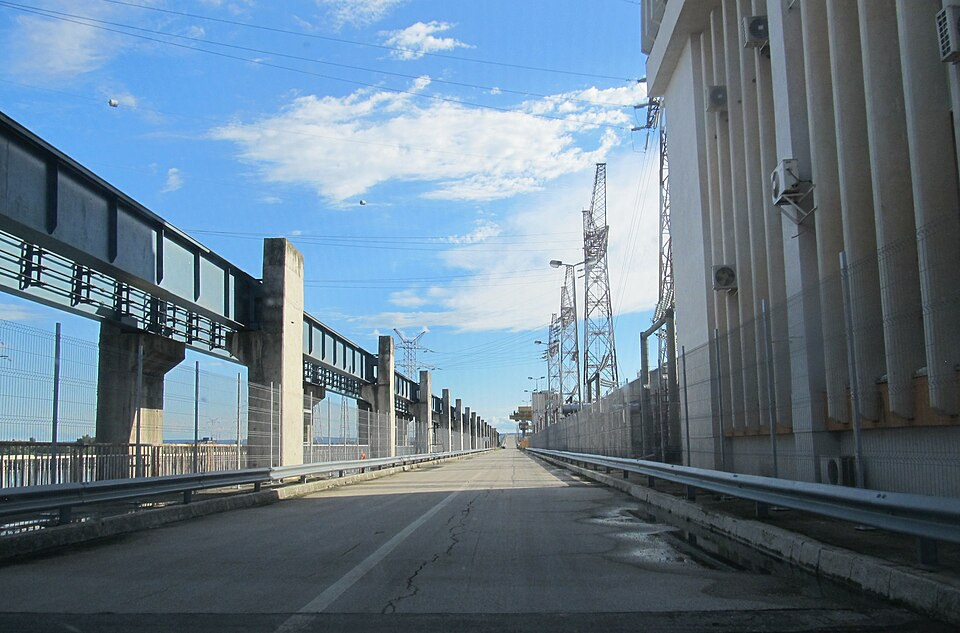
\includegraphics[height=0.30\textheight]{ch4_portile_de_fier_ii.jpg}\\[1mm]
\imgcap{Hidrocentrala Porțile de Fier II, pe Dunăre}
\imgcredit{https://commons.wikimedia.org/wiki/File:Por\%C8\%9Bile_de_Fier_II_(01).jpg}{Foto: Nenea hartia (2016); CC BY-SA 4.0; Wikimedia Commons}
\end{column}
\end{columns}
\end{frame}

\begin{frame}{Consumul orar: ziua și săptămîna}
\itemsize{\footnotesize}
\begin{center}
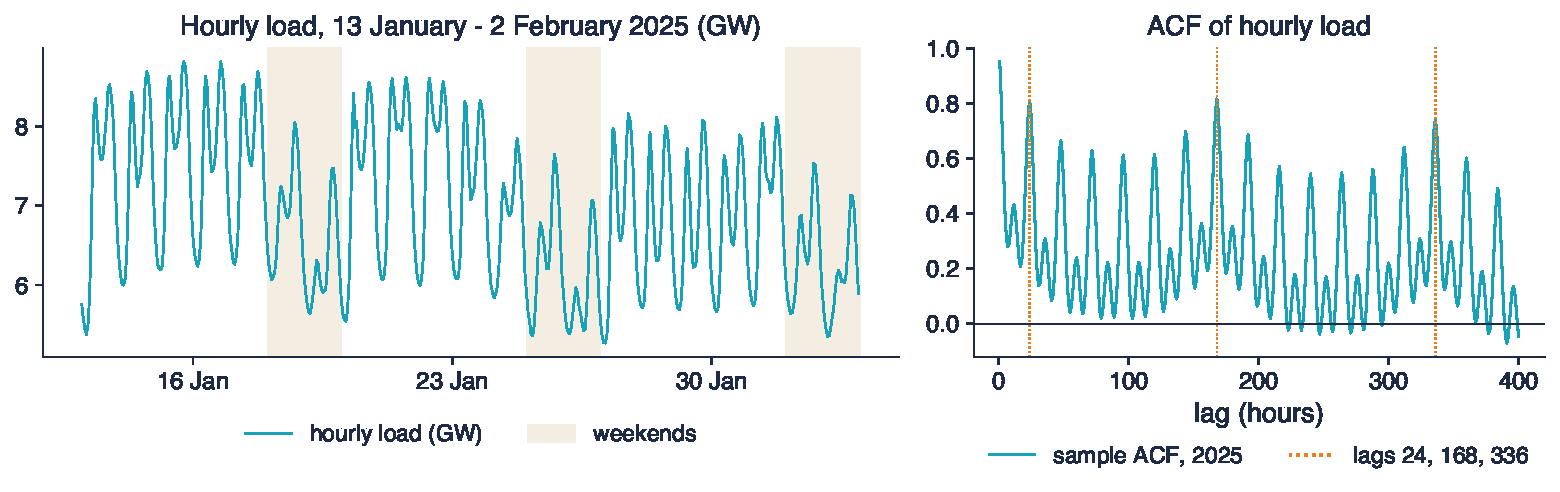
\includegraphics[width=0.97\textwidth,height=0.56\textheight,keepaspectratio]{tsa_ch4_load_hourly.pdf}
\end{center}
\vspace{-0.25cm}
\begin{itemize}
    \item Stînga: trei săptămîni din ianuarie 2025; dreapta: ACF de selecție pentru toate orele din 2025, pînă la lagul 400
\end{itemize}
\quantlet{TSA\_ch4\_multiple\_seasonality}{\qlurl{TSA_ch4_multiple_seasonality}}
\end{frame}

\begin{frame}{Interpretarea consumului orar}
\itemsize{\footnotesize}
\begin{itemize}
    \item Ciclul zilnic: minimul în jurul orei 3:00 (în medie 5{,}3 GW în 2025), maximul în jurul orei 19:00 (7{,}3 GW)
    \begin{itemize}
        \item ACF $0{,}81$ la lagul 24, $0{,}43$ la lagul 12
    \end{itemize}
    \item Ciclul săptămînal: weekendurile sînt mai joase; ACF $0{,}82$ la lagul 168 (o săptămînă), peste valoarea de la lagul 24
    \begin{itemize}
        \item aceeași oră de acum o săptămînă este cel mai bun predictor individual: lunea seamănă cu lunea trecută, nu cu duminica
    \end{itemize}
    \item Și un ciclu anual peste acestea (încălzire și aer condiționat): trei perioade, 24, 168 și aproximativ 8766 de ore
    \item SARIMA nu este suficient: are o singură perioadă întreagă $s$, în timp ce aici acționează simultan $s = 24$, $168$ și $8766$
    \begin{itemize}
        \item un polinom în $L^{168}$ este lent și instabil, 365,25 nu este un număr întreg, iar sărbătorile rup tiparul săptămînal
        \item răspunsuri: MSTL, regresia armonică dinamică (DHR), TBATS, Prophet
    \end{itemize}
\end{itemize}
\end{frame}

\begin{frame}{MSTL: cîte o componentă sezonieră pentru fiecare perioadă}
\itemsize{\footnotesize}
\begin{center}
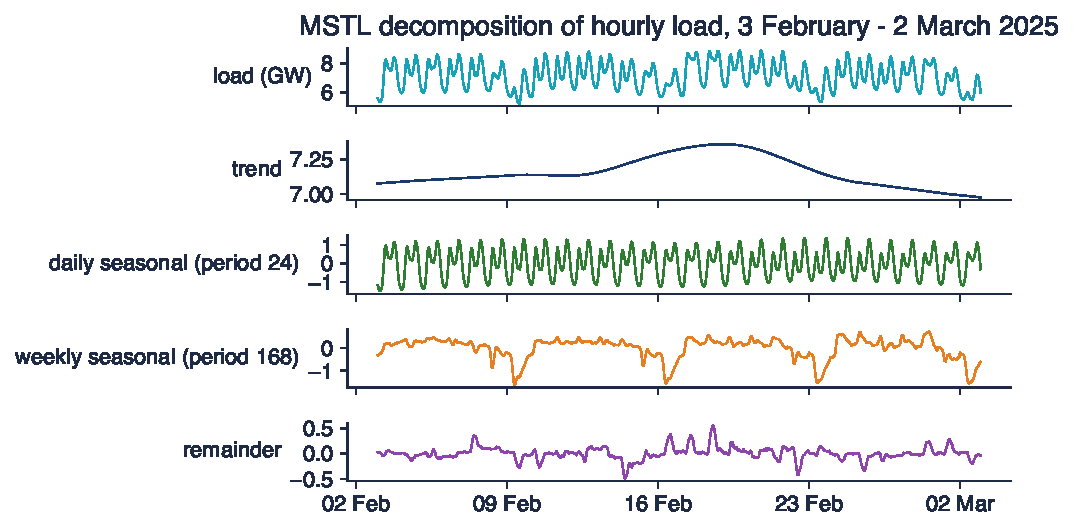
\includegraphics[width=0.97\textwidth,height=0.64\textheight,keepaspectratio]{tsa_ch4_mstl.pdf}
\end{center}
\vspace{-0.25cm}
\begin{itemize}
    \item MSTL (\refMSTL) aplică STL (\tsachlink{https://danpele.github.io/Time-Series-Analysis/RO/Cursuri/capitol0_introducere.pdf}{Capitolul 0}) în mod repetat, cîte o dată pentru fiecare perioadă (24 și 168 de ore), pînă cînd componentele se stabilizează
\end{itemize}
\quantlet{TSA\_ch4\_multiple\_seasonality}{\qlurl{TSA_ch4_multiple_seasonality}}
\end{frame}

\begin{frame}{Interpretarea descompunerii MSTL}
\itemsize{\small}
\begin{itemize}
    \item Din varianța în jurul trendului: 70\% componenta zilnică, 29\% componenta săptămînală, 2\% componenta neregulată
    \begin{itemize}
        \item amplitudinea componentei zilnice în prima săptămînă: 2{,}8 GW; a celei săptămînale: 2{,}1 GW
    \end{itemize}
    \item Componenta săptămînală este plată de luni pînă vineri și scade sîmbăta și mai mult duminica
    \item Componenta neregulată este mică, dar nu este zgomot alb: valuri de frig și sărbători; un model de prognoză adaugă dinamică și regresori
\end{itemize}
\end{frame}

\begin{frame}{Consumul zilnic și sărbătorile legale}
\itemsize{\footnotesize}
\begin{center}
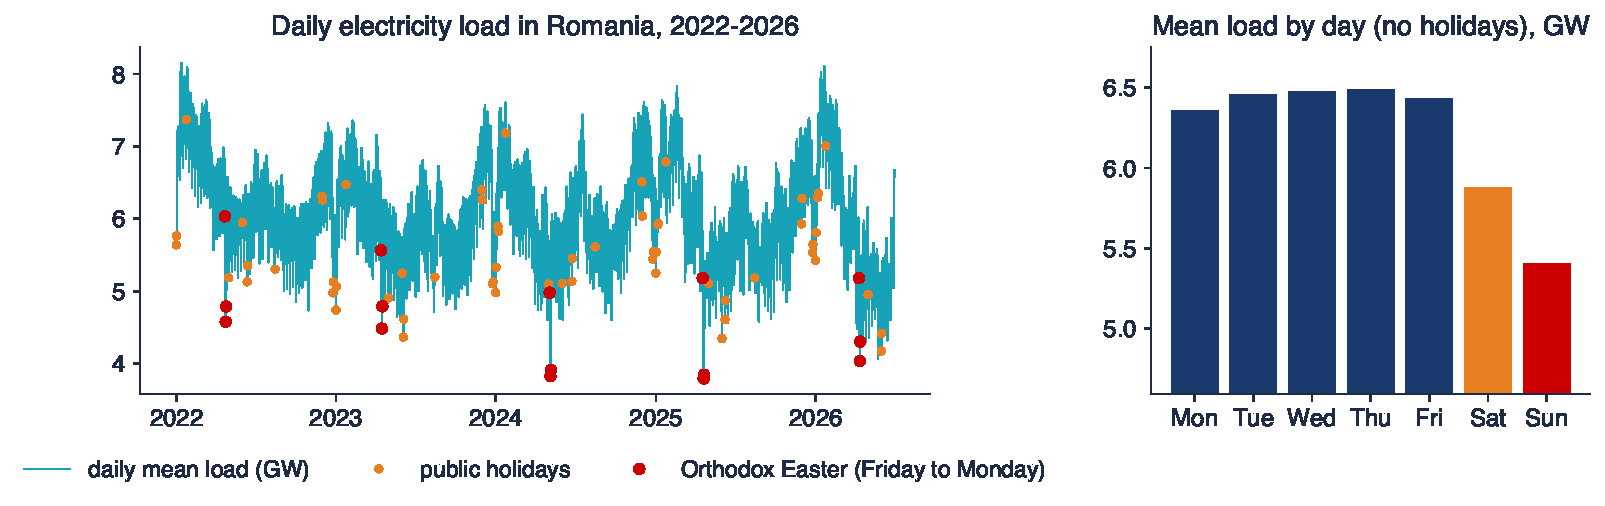
\includegraphics[width=0.97\textwidth,height=0.56\textheight,keepaspectratio]{tsa_ch4_load_daily.pdf}
\end{center}
\vspace{-0.25cm}
\begin{itemize}
    \item Consumul mediu zilnic, 2022--2026, 1\,642 de zile; sărbătorile legale marcate; dreapta: media pe zile ale săptămînii, fără sărbători
\end{itemize}
\quantlet{TSA\_ch4\_multiple\_seasonality}{\qlurl{TSA_ch4_multiple_seasonality}}
\end{frame}

\begin{frame}{Interpretarea consumului zilnic}
\itemsize{\small}
\begin{itemize}
    \item Săptămîna: sîmbăta cu 9\%, iar duminica cu 17\% sub miercuri
    \begin{itemize}
        \item Anul: ianuarie cu 25\% peste mai; un vîrf mai mic vara (aerul condiționat)
    \end{itemize}
    \item Sărbătorile: cea mai joasă zi din eșantion este Duminica Paștelui, 20 aprilie 2025 (3{,}79 GW, media 6{,}18 GW)
    \begin{itemize}
        \item cele patru zile de Paște (vineri--luni) au în medie 4{,}62 GW; perioada Crăciun--Anul Nou este și ea joasă
    \end{itemize}
    \item Nivelul scade în 2022--2026; cauze posibile: șocul de preț din 2022 și panourile solare de pe acoperișuri, care acoperă o parte din cerere fără a trece prin rețea
\end{itemize}
\end{frame}

\begin{frame}{O regresie armonică dinamică pentru consumul zilnic}
\itemsize{\footnotesize}
\begin{itemize}
    \item $y_t = \sum_{k=1}^{4}\left[\alpha_k\sin\frac{2\pi kt}{365{,}25} + \beta_k\cos\frac{2\pi kt}{365{,}25}\right] + \sum_{j}\delta_jD^{\mathrm{zi}}_{jt} + \lambda_1H_t + \lambda_2E_t + \lambda_3X_t + u_t$
    \begin{itemize}
        \item $\alpha_k, \beta_k$: coeficienții Fourier anuali; $\delta_j$: efectul zilei $j$ față de duminică; $\lambda_1, \lambda_2, \lambda_3$: efectele zilelor speciale, în GW
        \item termeni Fourier anuali; variabile dummy pentru zilele săptămînii (duminica este baza); $H$ sărbătoare legală, $E$ Paște (vineri--luni), $X$ 24 decembrie -- 2 ianuarie
        \item $u_t \sim$ ARIMA(1,1,1), ales cu AIC: \textbf{regresia armonică dinamică} (DHR, \refFPPdhr)
    \end{itemize}
    \item Estimările, cu datele pînă la prima origine de prognoză (30 iunie 2025), în GW:
    \begin{itemize}
        \item miercuri $+1{,}08$, luni $+0{,}88$, sîmbătă $+0{,}50$ față de duminică
        \item sărbătoare legală $-0{,}38$ (eroarea standard 0{,}02), Paștele încă $-0{,}58$, Crăciun--Anul Nou $-0{,}61$
        \item erori: AR $0{,}80$, MA $\ensuremath{-}0{,}98$, $\hat\sigma = 186$ MW; Ljung--Box(14) p $<$\,0{,}001: rămîne puțină dinamică
    \end{itemize}
\end{itemize}
\end{frame}

\begin{frame}{Recapitulare: sezonalitatea multiplă}
\itemsize{\small}
\begin{itemize}
    \item Consumul orar are cicluri zilnice, săptămînale și anuale; consumul zilnic are cicluri săptămînale și anuale
    \item SARIMA tratează o singură perioadă întreagă; MSTL descompune mai multe
    \item Sărbătorile, mai ales Paștele, sînt cele mai mari abateri: au nevoie de regresori
    \item DHR = termeni Fourier + variabile dummy de calendar + erori ARIMA: flexibilă și transparentă
\end{itemize}
\end{frame}


%=============================================================================
\section{TBATS și Prophet}
%=============================================================================

\begin{frame}{TBATS}
\itemsize{\footnotesize}
\begin{itemize}
    \item \refTBATS: netezire exponențială (ETS, \tsachlink{https://danpele.github.io/Time-Series-Analysis/RO/Cursuri/capitol0_introducere.pdf}{Capitolul 0}) pentru sezonalitate complexă; numele enumeră părțile modelului
    \begin{itemize}
        \item sezonalitate trigonometrică (T), transformare Box--Cox (B), erori ARMA (A), trend (T), componente sezoniere (S)
    \end{itemize}
    \item $y_t^{(\omega)} = \ell_{t-1} + \phi b_{t-1} + \sum_{i}s^{(i)}_{t-1} + d_t$, $d_t$ ARMA($p,q$); nivelul și trendul se actualizează ca în metoda Holt
    \begin{itemize}
        \item $y_t^{(\omega)}$: seria după o transformare Box--Cox cu parametrul $\omega$; $\ell_t$: nivelul; $b_t$: panta; $\phi$: factorul de amortizare; $s^{(i)}_t$: componenta sezonieră $i$
        \item fiecare perioadă $m_i$ are $K_i$ armonici $s^{(i)}_{j,t}$, fiecare o pereche rotitoare (cosinus, sinus) actualizată de erori: un tipar Fourier care poate evolua
    \end{itemize}
    \item Alegeri automate cu AIC: Box--Cox sau nu, trend, trend amortizat sau fără trend, valorile $K_i$, ordinele ARMA
    \begin{itemize}
        \item consumul zilnic pînă în iunie 2025, perioadele 7 și 365,25 (fără Box--Cox, fără trend): $K = 3$ armonici săptămînale și $K = 9$ anuale, ARMA(1,2), 28 de stări
    \end{itemize}
    \item Limite: fără regresori, deci fără sărbători sau Paște; lent pe serii lungi; pachetul Python \texttt{tbats}
\end{itemize}
\end{frame}

\begin{frame}{Prophet}
\itemsize{\footnotesize}
\begin{itemize}
    \item \refProphet{} (Meta): o regresie în timp, $y(t) = g(t) + s(t) + h(t) + \varepsilon_t$
    \begin{itemize}
        \item $g(t)$: trend liniar pe porțiuni (sau logistic) a cărui pantă se poate schimba în \textbf{puncte de schimbare}; o distribuție a priori Laplace aduce cele mai multe schimbări la zero
        \item $s(t)$: termeni Fourier, implicit $K = 10$ pentru an și $K = 3$ pentru săptămînă
        \item $h(t)$: un efect pentru fiecare sărbătoare (cu ferestre opționale în jurul ei), dintr-o listă de date
    \end{itemize}
    \item Estimat cu Stan (maximul a posteriori); intervalele simulează punctele de schimbare viitoare și zgomotul
    \begin{itemize}
        \item fără parte autoregresivă: eroarea de azi nu modifică prognoza de mîine
    \end{itemize}
    \item Construit pentru multe serii economice cu efecte puternice de calendar și date lipsă; pachetul Python \texttt{prophet}
\end{itemize}
\end{frame}

\begin{frame}{Componentele Prophet pentru consumul zilnic}
\itemsize{\footnotesize}
\begin{center}
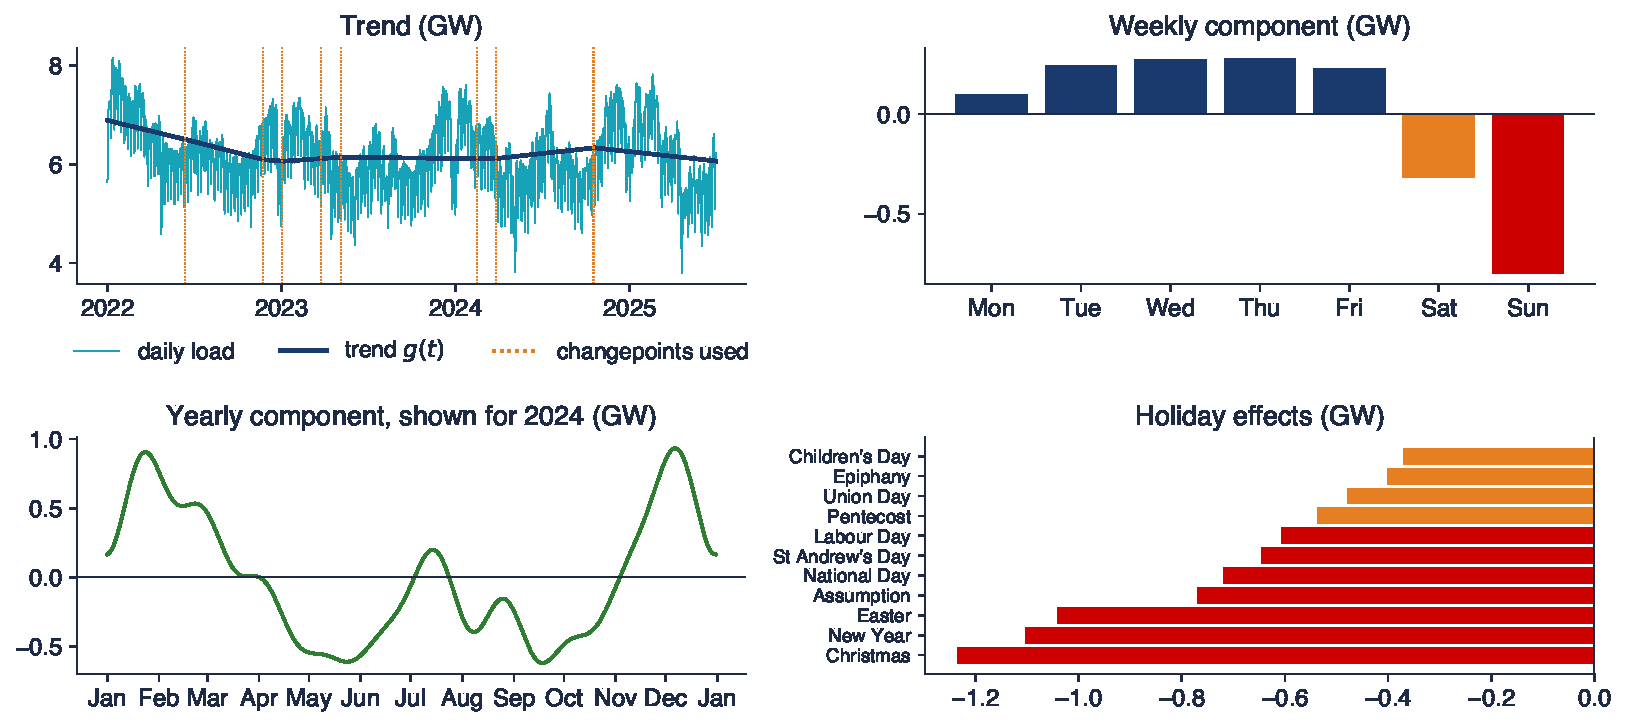
\includegraphics[width=0.97\textwidth,height=0.64\textheight,keepaspectratio]{tsa_ch4_prophet.pdf}
\end{center}
\vspace{-0.25cm}
\begin{itemize}
    \item Prophet cu sărbătorile legale din România, consumul zilnic 2022 -- iunie 2025
\end{itemize}
\quantlet{TSA\_ch4\_tbats\_prophet}{\qlurl{TSA_ch4_tbats_prophet}}
\end{frame}

\begin{frame}{Interpretarea componentelor Prophet}
\itemsize{\small}
\begin{itemize}
    \item Trendul de la 6{,}89 la 6{,}07 GW, mai plat după 2023; 25 de puncte de schimbare candidate, cele mai multe aduse la zero
    \begin{itemize}
        \item săptămînal: miercuri $+0{,}27$, sîmbătă $\ensuremath{-}0{,}32$, duminică $\ensuremath{-}0{,}80$ GW
    \end{itemize}
    \item Anual: maximul la începutul lui decembrie ($+0{,}93$ GW, 7 decembrie 2024), minimul la mijlocul lui septembrie ($\ensuremath{-}0{,}62$ GW, 18 septembrie 2024), arătat pentru 2024
    \item Sărbătorile: Crăciunul $\ensuremath{-}1{,}24$, Anul Nou $\ensuremath{-}1{,}10$, Paștele $\ensuremath{-}1{,}04$ GW; Ziua Copilului doar $\ensuremath{-}0{,}37$ GW
    \item Fiecare componentă poate fi citită și verificată cu ceea ce știm despre economie
\end{itemize}
\end{frame}

\begin{frame}{Recapitulare: DHR, TBATS și Prophet comparate}
\itemsize{\footnotesize}
\begin{center}
\scriptsize
\begin{tabular}{>{\raggedright\arraybackslash}p{2.6cm}>{\raggedright\arraybackslash}p{2.8cm}>{\raggedright\arraybackslash}p{2.8cm}>{\raggedright\arraybackslash}p{2.8cm}}
\toprule
 & \textbf{DHR} & \textbf{TBATS} & \textbf{Prophet} \\
\midrule
Sezonalitatea & Fourier, fixă & Fourier, evolutivă & Fourier, fixă \\
Mai multe perioade & da & da & da \\
Sărbători, regresori & da & nu & da \\
Dinamica pe termen scurt & erori ARMA & erori ARMA & niciuna \\
Trendul & prin erori (ARIMA) & local (Holt) & liniar pe porțiuni \\
Viteza & rapidă & lentă & rapidă \\
\bottomrule
\end{tabular}
\end{center}
\begin{itemize}
    \item În esență, toate trei sînt regresii pe sinusuri și cosinusuri; diferă prin ceea ce mai modelează
    \item Care dintre ele prognozează mai bine este o întrebare empirică: secțiunea următoare îi răspunde în afara eșantionului
\end{itemize}
\end{frame}


%=============================================================================
\section{Evaluarea prognozelor}
%=============================================================================

\begin{frame}{Validarea încrucișată pentru serii de timp}
\itemsize{\footnotesize}
\begin{center}
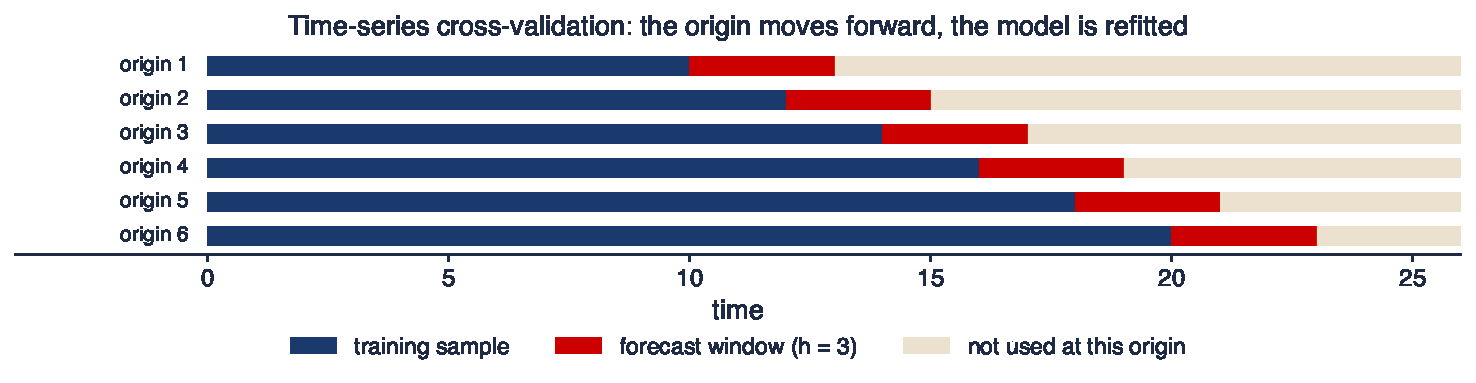
\includegraphics[width=0.97\textwidth,height=0.40\textheight,keepaspectratio]{tsa_ch4_cv_scheme.pdf}
\end{center}
\vspace{-0.25cm}
\begin{itemize}
    \item Origine de prognoză mobilă (\refTashman; \refFPPcv): estimăm pe datele pînă la origine, prognozăm $h$ pași, mutăm originea, reestimăm
    \item Fereastră care se extinde (în figură) sau fereastră glisantă de lungime fixă; nu folosim niciodată date viitoare la estimare
\end{itemize}
\quantlet{TSA\_ch4\_evaluation}{\qlurl{TSA_ch4_evaluation}}
\end{frame}

\begin{frame}{Interpretarea schemei de evaluare}
\itemsize{\footnotesize}
\begin{itemize}
    \item Consumul zilnic: 26 de origini la 14 zile, de la 30 iunie 2025 la 15 iunie 2026; orizontul $h = 14$ zile
    \begin{itemize}
        \item un an de prognoze în afara eșantionului, toate anotimpurile și toate sărbătorile, inclusiv Paștele din 2026
    \end{itemize}
    \item Șapte metode, toate reestimate la fiecare origine
    \begin{itemize}
        \item sezonieră naivă (perioada 7); ETS (Holt--Winters, trend amortizat, perioada 7); SARIMA(2,0,1)$(0,1,1)_7$; DHR; TBATS; Prophet
        \item Combinarea: media simplă a prognozelor celor cinci modele (toate, cu excepția celei sezoniere naive)
    \end{itemize}
    \item Ordinele SARIMA și ale erorilor DHR se aleg o singură dată, cu AIC, pe datele dinaintea primei origini: fără a privi perioada de test
    \item Validarea încrucișată care ignoră ordinea în timp (grupuri aleatoare) este validă doar pentru autoregresii pure cu erori de tip zgomot alb (\refBHK)
\end{itemize}
\end{frame}

\begin{frame}{Testul Diebold--Mariano}
\itemsize{\footnotesize}
\begin{itemize}
    \item \refDM: este diferența de acuratețe dintre două prognoze mai mare decît ar rezulta din întîmplare?
    \begin{itemize}
        \item $e_{1t}$, $e_{2t}$: erorile celor două prognoze; $L$: funcția de pierdere
        \item diferența de pierdere $d_t = L(e_{1t}) - L(e_{2t})$, $L(e) = e^2$ sau $|e|$; $H_0$: $E[d_t] = 0$
    \end{itemize}
    \item $\mathrm{DM} = \dfrac{\bar d}{\sqrt{\hat V/n}}$, $\hat V = \hat\gamma_d(0) + 2\sum_{k=1}^{h-1}\hat\gamma_d(k)$
    \begin{itemize}
        \item $\bar d$: media celor $n$ diferențe; $\hat\gamma_d(k)$: autocovarianța lor la lagul $k$; un DM negativ favorizează prognoza 1
        \item erorile la $h$ pași se suprapun, deci $d_t$ este autocorelat pînă la lagul $h - 1$
        \item asimptotic $N(0, 1)$; eșantioane mici: $\mathrm{HLN} = \sqrt{\frac{n + 1 - 2h + h(h - 1)/n}{n}}\;\mathrm{DM}$, comparat cu $t(n - 1)$ (\refHLN)
    \end{itemize}
    \item Schema noastră: o valoare pe origine, $d_j$ = diferența medie de pierdere în fereastra de 14 zile; ferestrele nu se suprapun, deci $h = 1$ în formulă
    \begin{itemize}
        \item testul compară prognoze, nu modele: zgomotul reestimării face parte din ceea ce se testează
    \end{itemize}
\end{itemize}
\end{frame}

\begin{frame}{Exemplu rezolvat: un test Diebold--Mariano}
\itemsize{\small}
\begin{itemize}
    \item Cinci ferestre; diferențele medii ale erorilor pătratice, metoda 1 minus metoda 2: $-0{,}30; 0{,}10; -0{,}50; -0{,}20; -0{,}40$
    \begin{itemize}
        \item $\bar d = \ensuremath{-}0{,}26$: metoda 1 are pierderi mai mici în patru ferestre din cinci
    \end{itemize}
    \item $\hat\gamma_d(0) = \frac15\sum(d_j - \bar d)^2 = 0{,}042$
    \begin{itemize}
        \item $\mathrm{DM} = \ensuremath{-}0{,}26/\sqrt{0{,}042/5} = \ensuremath{-}2{,}82$; $\mathrm{HLN} = \sqrt{4/5}\cdot\mathrm{DM} = \ensuremath{-}2{,}53$
    \end{itemize}
    \item $|\ensuremath{-}2{,}53| < t_{0{,}975}(4) = 2{,}78$ (p = 0{,}065): acuratețea egală nu se respinge la 5\%
    \begin{itemize}
        \item valoarea critică a distribuției Normale, 1,96, ar fi dus la respingere: cu puține ferestre, corecția contează
    \end{itemize}
\end{itemize}
\end{frame}

\begin{frame}{Prognoze dintr-o singură origine, peste Paștele din 2026}
\itemsize{\footnotesize}
\begin{center}
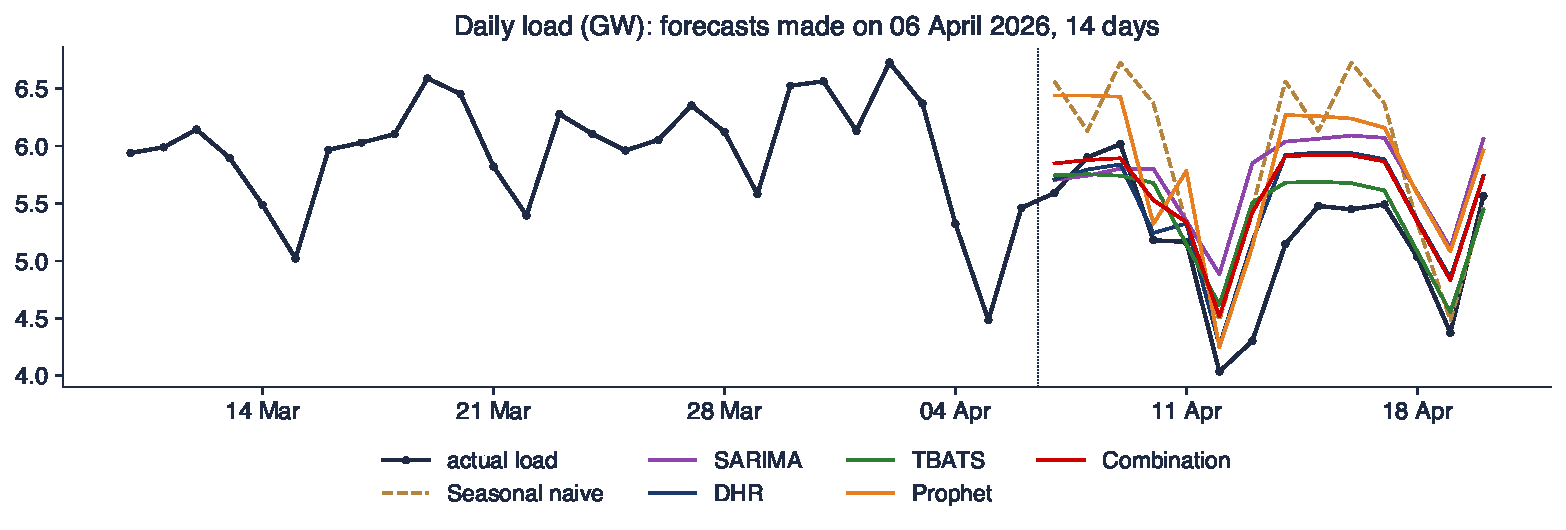
\includegraphics[width=0.97\textwidth,height=0.56\textheight,keepaspectratio]{tsa_ch4_load_fc.pdf}
\end{center}
\vspace{-0.25cm}
\begin{itemize}
    \item Originea 6 aprilie 2026, 14 zile înainte; Duminica Paștelui ortodox a fost pe 12 aprilie 2026
\end{itemize}
\quantlet{TSA\_ch4\_evaluation}{\qlurl{TSA_ch4_evaluation}}
\end{frame}

\begin{frame}{Interpretarea unei ferestre de prognoză}
\itemsize{\small}
\begin{itemize}
    \item MAE în această fereastră (MW): ETS 299, TBATS 309, DHR 344, Combinarea 394, SARIMA 584, Prophet 616, sezonieră naivă 686
    \begin{itemize}
        \item metoda sezonieră naivă copiază săptămîna normală anterioară în săptămîna Paștelui
    \end{itemize}
    \item Toate modelele văd scăderea de duminică; DHR și Prophet coboară și Vinerea Mare și a doua zi de Paște, pe care modelele săptămînale le tratează ca zile lucrătoare
    \item După Paște, consumul rămîne sub toate prognozele pînă la sfîrșitul săptămînii; ETS și TBATS, al căror nivel urmează ultimele zile, au aici erorile cele mai mici
    \item O singură fereastră este un caz izolat; slide-urile următoare fac media pe toate cele 26 de ferestre
\end{itemize}
\end{frame}

\begin{frame}{Rezultatele validării încrucișate pentru consumul zilnic}
\itemsize{\footnotesize}
\begin{center}
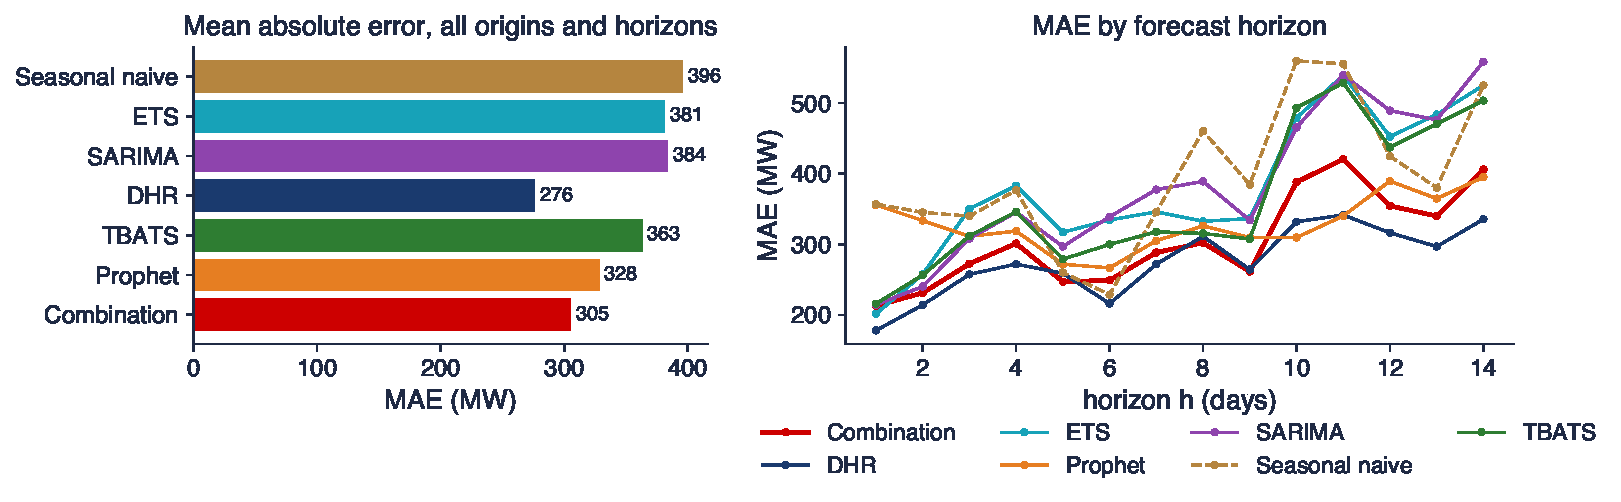
\includegraphics[width=0.97\textwidth,height=0.56\textheight,keepaspectratio]{tsa_ch4_cv_results.pdf}
\end{center}
\vspace{-0.25cm}
\begin{itemize}
    \item 26 de origini $\times$ 14 orizonturi pentru fiecare metodă; stînga: MAE totală; dreapta: MAE pe orizonturi
\end{itemize}
\quantlet{TSA\_ch4\_evaluation}{\qlurl{TSA_ch4_evaluation}}
\end{frame}

\begin{frame}{Interpretarea rezultatelor validării încrucișate}
\itemsize{\footnotesize}
\begin{center}
\scriptsize
\begin{tabular}{lrrrrr}
\toprule
\textbf{Metoda} & \textbf{MAE} & \textbf{RMSE} & \textbf{MASE} & \textbf{DM față de s. naivă} & \textbf{DM față de DHR} \\
\midrule
Sezonieră naivă & 396 & 529 & 1{,}28 & -- & $4{,}42$ ($<$\,0{,}001) \\
ETS & 381 & 492 & 1{,}23 & $\ensuremath{-}0{,}80$ (0{,}431) & $3{,}08$ (0{,}005) \\
SARIMA & 384 & 477 & 1{,}24 & $\ensuremath{-}1{,}23$ (0{,}231) & $3{,}29$ (0{,}003) \\
DHR & \textbf{276} & \textbf{350} & \textbf{0{,}89} & $\ensuremath{-}4{,}42$ ($<$\,0{,}001) & -- \\
TBATS & 363 & 468 & 1{,}18 & $\ensuremath{-}1{,}50$ (0{,}145) & $3{,}02$ (0{,}006) \\
Prophet & 328 & 412 & 1{,}06 & $\ensuremath{-}2{,}99$ (0{,}006) & $2{,}76$ (0{,}011) \\
Combinarea & 305 & 380 & 0{,}99 & $\ensuremath{-}3{,}82$ ($<$\,0{,}001) & $1{,}89$ (0{,}070) \\
\bottomrule
\end{tabular}
\end{center}
\begin{itemize}
    \item MAE și RMSE în MW; MASE (\refHKo) = MAE / 309 MW, MAE în eșantion a metodei sezoniere naive săptămînale; DM: statistica HLN (p-value-ul) pe media erorilor pătratice din fiecare fereastră, metoda de pe rînd minus metoda de pe coloană
    \item DHR cîștigă; împreună cu combinarea, este singura metodă cu MASE sub 1; Prophet este al doilea model individual: singurele două care includ sărbătorile
    \item ETS, SARIMA și TBATS nu sînt semnificativ mai bune decît metoda sezonieră naivă
\end{itemize}
\end{frame}

\begin{frame}{Un al doilea test: PIB-ul României}
\itemsize{\footnotesize}
\begin{center}
\scriptsize
\begin{tabular}{lrrrr}
\toprule
\textbf{Metoda} & MAE, $h = 1$ & MAE, $h = 4$ & fără 2019--2020, $h = 1$ & fără 2019--2020, $h = 4$ \\
\midrule
SARIMA (airline) & 1{,}69 & 2{,}70 & 1{,}32 & 1{,}89 \\
ETS & 1{,}76 & 2{,}84 & 1{,}41 & 2{,}44 \\
Sezonieră naivă & 3{,}81 & 3{,}74 & 3{,}80 & 3{,}49 \\
Combinarea (SARIMA, ETS) & 1{,}70 & 2{,}65 & 1{,}34 & 2{,}02 \\
\bottomrule
\end{tabular}
\end{center}
\begin{itemize}
    \item $100\ln Y$, erori în \%; 51 de origini trimestriale, T4 2012--T2 2025, fereastră care se extinde; 43 de origini fără 2019--2020
    \item DM (HLN), SARIMA față de ETS: $h = 1$: $\ensuremath{-}1{,}46$ (p = 0{,}150); $h = 4$: $0{,}50$ (p = 0{,}620)
    \item SARIMA față de metoda sezonieră naivă: $h = 1$: $\ensuremath{-}4{,}00$ (p $<$\,0{,}001); $h = 4$: $\ensuremath{-}0{,}54$ (p = 0{,}591)
    \item La un an înainte, erorile din pandemie domină și nicio diferență nu este semnificativă; fără ele, SARIMA are cea mai mică MAE la $h = 4$
\end{itemize}
\end{frame}

\begin{frame}{Recapitulare: evaluarea prognozelor}
\itemsize{\small}
\begin{itemize}
    \item Evaluați în afara eșantionului, cu origini mobile; alegeți ordinele modelelor înaintea perioadei de test
    \item MASE compară cu metoda sezonieră naivă și între serii
    \item Testul DM (cu corecția HLN) arată dacă un cîștig este mai mult decît un efect al întîmplării
    \item Consumul zilnic: modelele care includ calendarul (DHR, Prophet) cîștigă; pentru PIB, SARIMA și ETS sînt apropiate
\end{itemize}
\end{frame}


%=============================================================================
\section{Combinarea prognozelor}
%=============================================================================

\begin{frame}{Avantajul combinării prognozelor}
\itemsize{\footnotesize}
\begin{itemize}
    \item \refBG: o medie ponderată a două prognoze nedeplasate, $f_c = wf_1 + (1 - w)f_2$
    \begin{itemize}
        \item $w$: ponderea prognozei 1; $\sigma_1$, $\sigma_2$: abaterile standard ale celor două erori; $\rho$: corelația lor
        \item $\mathrm{MSE}(w) = w^2\sigma_1^2 + (1 - w)^2\sigma_2^2 + 2w(1 - w)\rho\sigma_1\sigma_2$
        \item ponderea optimă $w^* = \dfrac{\sigma_2^2 - \rho\sigma_1\sigma_2}{\sigma_1^2 + \sigma_2^2 - 2\rho\sigma_1\sigma_2}$; cîștigul este mare cînd $\rho$ este mic
    \end{itemize}
    \item Exemplu: $\sigma_1 = 1$, $\sigma_2 = 1{,}2$, $\rho = 0{,}75$: $\mathrm{MSE}(0{,}5) = 1{,}060$; $w^* = 0{,}84$, $\mathrm{MSE}(w^*) = 0{,}984$
    \begin{itemize}
        \item erori puternic corelate: media cu ponderi egale este mai slabă decît prognoza mai bună ($\sigma_1^2 = 1$), iar chiar ponderea optimă cîștigă puțin
    \end{itemize}
    \item \textbf{Paradoxul combinării prognozelor} (\refSW; \refSmithWallis): ponderile estimate sînt rareori mai bune decît ponderile egale
    \begin{itemize}
        \item ponderile trebuie estimate, iar eroarea lor de estimare consumă cîștigul teoretic
    \end{itemize}
\end{itemize}
\end{frame}

\begin{frame}{Combinarea DHR și Prophet}
\itemsize{\footnotesize}
\begin{center}
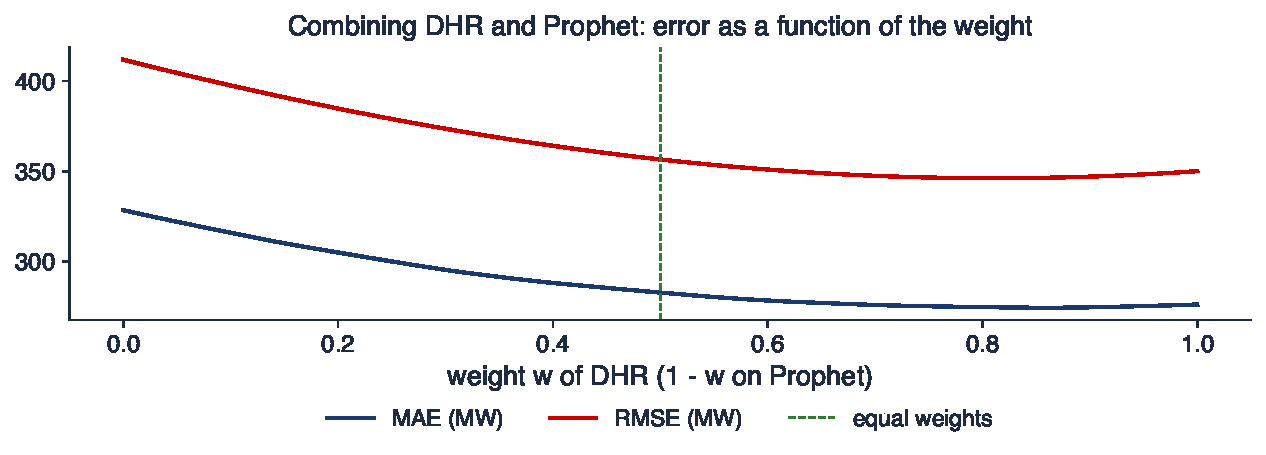
\includegraphics[width=0.97\textwidth,height=0.52\textheight,keepaspectratio]{tsa_ch4_combination.pdf}
\end{center}
\vspace{-0.25cm}
\begin{itemize}
    \item Erorile din validarea încrucișată pentru consumul zilnic; $w$ este ponderea DHR
\end{itemize}
\quantlet{TSA\_ch4\_evaluation}{\qlurl{TSA_ch4_evaluation}}
\end{frame}

\begin{frame}{Interpretarea combinării}
\itemsize{\footnotesize}
\begin{itemize}
    \item MAE: doar Prophet (w = 0) 328 MW, doar DHR (w = 1) 276 MW, ponderi egale 283 MW
    \begin{itemize}
        \item cea mai bună retrospectiv: $w = 0{,}86$, MAE 274 MW, un cîștig mic ales după ce am văzut datele de test
    \end{itemize}
    \item Erorile celor două metode sînt puternic corelate ($\rho = 0{,}75$): ambele ratează aceleași valuri de frig
    \item Media celor cinci modele (MAE 305) este a doua, după DHR, și mai bună decît patru dintre cele cinci componente: o asigurare ieftină cînd cîștigătorul nu este cunoscut dinainte
    \item În competiția M4 (\refMFour), cele mai multe dintre metodele de top au fost combinații; o sinteză: \refWangComb
\end{itemize}
\end{frame}


%=============================================================================
\section{Contribuția posibilă a AI}
%=============================================================================

\begin{frame}{Contribuția posibilă a AI}
\itemsize{\small}
\begin{itemize}
    \item \textbf{Cod}: o primă versiune a unei bucle cu origini mobile care reestimează SARIMA, DHR, TBATS și Prophet și păstrează erorile pe orizonturi
    \item \textbf{Calendare}: liste de sărbători și sărbători mobile pentru alte țări, care trebuie verificate cu sursele oficiale
    \item \textbf{Explicații}: o a doua deducere a ACF pentru modelul airline sau a funcției de prognoză pe termen lung
    \item Exemplu de prompt
    \begin{itemize}
        \item \aiprompt{Write Python code that forecasts daily electricity load 14 days ahead with a regression on annual Fourier terms, weekday dummies and Romanian public holidays (Orthodox Easter from dateutil) with ARMA errors, and evaluates it against SARIMA by rolling origins and a Diebold-Mariano test.}
    \end{itemize}
\end{itemize}
\end{frame}

\begin{frame}{Verificări necesare}
\itemsize{\small}
\begin{itemize}
    \item Data Paștelui: ortodox, nu occidental (\texttt{EASTER\_ORTHODOX}); în 2024 cele două diferă cu cinci săptămîni
    \item Fără informații din viitor: variabilele, ordinele modelelor și listele de sărbători trebuie să fie disponibile la fiecare origine
    \item Convențiile de semn pentru $\theta$ și $\Theta$ în program și gradele de libertate ale testului Ljung--Box
    \item Date ajustate sau neajustate: SARIMA pe NSA; ratele de creștere pe varianta potrivită
    \item Că testul DM folosește pierderile din aceleași ferestre pentru ambele metode și corecția HLN pentru $n$ mic
    \item Fiecare referință citată: trebuie să existe; verificați DOI-ul
\end{itemize}
\end{frame}


%=============================================================================
\section{Rezumat}
%=============================================================================

\begin{frame}{Idei de reținut}
\itemsize{\small}
\begin{itemize}
    \item Sezonalitatea se repetă cu o perioadă cunoscută; poate fi deterministă (variabile dummy, Fourier) sau stochastică ($\Delta_s$)
    \item SARIMA înmulțește polinoame obișnuite și sezoniere; modelul airline se potrivește multor serii, cu doi parametri
    \item Datele oficiale: SCA pentru creșterea pe termen scurt, NSA cu regresori de calendar pentru prognoza SARIMA
    \item Efectele de calendar (zile lucrătoare, Paștele ortodox, sărbători) sînt cunoscute dinainte și contează adesea mai mult decît clasa de modele
    \item Sezonalitatea multiplă: MSTL, DHR, TBATS, Prophet; pentru consumul zilnic din România, DHR cîștigă în afara eșantionului
    \item Judecați prognozele cu origini mobile, MASE și testul DM; combinați-le cînd cîștigătorul este incert
\end{itemize}
\end{frame}

\begin{frame}{Formule de reținut}
\itemsize{\small}
{\renewcommand{\arraystretch}{1.35}\begin{center}
\scriptsize
\begin{tabular}{ll}
\toprule
\textbf{Mărimea} & \textbf{Formula} \\
\midrule
Diferența sezonieră & $\Delta_sy_t = (1 - L^s)y_t$, \quad $\Delta\Delta_s = 1 - L - L^s + L^{s+1}$ \\
SARIMA & $\phi(L)\Phi(L^s)(1 - L)^d(1 - L^s)^Dy_t = \theta(L)\Theta(L^s)\varepsilon_t$ \\
Airline & $\rho_1 = \frac{\theta}{1 + \theta^2}$, \quad $\rho_s = \frac{\Theta}{1 + \Theta^2}$, \quad $\rho_{s \pm 1} = \rho_1\rho_s$ \\
Fourier & $\sum_{k=1}^{K}[\alpha_k\sin(2\pi kt/m) + \beta_k\cos(2\pi kt/m)]$ \\
Prophet & $y(t) = g(t) + s(t) + h(t) + \varepsilon_t$ \\
MASE & $\frac1h\sum|e_{T+j}| \,/\, \frac{1}{T - m}\sum|y_t - y_{t-m}|$ \\
DM & $\bar d/\sqrt{\hat V/n}$, \quad $d_t = L(e_{1t}) - L(e_{2t})$ \\
Combinarea & $w^* = \frac{\sigma_2^2 - \rho\sigma_1\sigma_2}{\sigma_1^2 + \sigma_2^2 - 2\rho\sigma_1\sigma_2}$ \\
\bottomrule
\end{tabular}
\end{center}
}
\end{frame}

\begin{frame}{Autoevaluare}
\itemsize{\footnotesize}
\begin{itemize}
    \item \textbf{Întrebare}: cîți parametri are SARIMA$(1,1,1)(0,1,1)_{12}$ și la ce laguri apare $\varepsilon$?
    \begin{itemize}
        \item \textbf{Răspuns}: $\phi, \theta, \Theta, \sigma^2$, patru; $\varepsilon$ la lagurile 0, 1, 12, 13 (ultimul cu coeficientul $\theta\Theta$)
    \end{itemize}
    \item \textbf{Întrebare}: PIB-ul neajustat scade cu 40\% din T4 în T1. Este o recesiune?
    \begin{itemize}
        \item \textbf{Răspuns}: nu; este tiparul sezonier; priviți seria SCA sau creșterea față de anul anterior
    \end{itemize}
    \item \textbf{Întrebare}: un test DM cu 26 de ferestre dă HLN $= -1{,}93$. Este prima prognoză semnificativ mai bună la 5\%?
    \begin{itemize}
        \item \textbf{Răspuns}: nu: $|-1{,}93| < t_{0{,}975}(25) = 2{,}06$; este mai bună în medie, dar nu semnificativ
    \end{itemize}
    \item \textbf{Idee de proiect}: prognozați consumul orar de electricitate din România cu o DHR (termeni Fourier zilnici, săptămînali și anuali, sărbători, temperatură), comparată cu TBATS, Prophet și o combinare, prin origini mobile și teste DM
    \begin{itemize}
        \item Urmează: \tsachlink{https://danpele.github.io/Time-Series-Analysis/RO/Cursuri/capitol5_volatilitate_conditionata_garch.pdf}{Capitolul 5}, volatilitatea condiționată: modelele ARCH și GARCH
    \end{itemize}
\end{itemize}
\end{frame}


%=============================================================================
\section{Bibliografie}
%=============================================================================

\begin{frame}{Bibliografie (1/2)}
\itemsize{\tiny}
\begin{itemize}
    \item Bandara, K., Hyndman, R. J., \& Bergmeir, C. (2025). MSTL: A seasonal-trend decomposition algorithm for time series with multiple seasonal patterns. \textit{International Journal of Operational Research}, 52(1), 79--98. \href{https://doi.org/10.1504/ijor.2025.143957}{doi:10.1504/ijor.2025.143957}
    \item Bates, J. M., \& Granger, C. W. J. (1969). The combination of forecasts. \textit{Journal of the Operational Research Society}, 20(4), 451--468. \href{https://doi.org/10.1057/jors.1969.103}{doi:10.1057/jors.1969.103}
    \item Bergmeir, C., Hyndman, R. J., \& Koo, B. (2018). A note on the validity of cross-validation for evaluating autoregressive time series prediction. \textit{Computational Statistics \& Data Analysis}, 120, 70--83. \href{https://doi.org/10.1016/j.csda.2017.11.003}{doi:10.1016/j.csda.2017.11.003}
    \item Box, G. E. P., \& Cox, D. R. (1964). An analysis of transformations. \textit{Journal of the Royal Statistical Society, Series B}, 26(2), 211--243. \href{https://doi.org/10.1111/j.2517-6161.1964.tb00553.x}{doi:10.1111/j.2517-6161.1964.tb00553.x}
    \item Box, G. E. P., Jenkins, G. M., \& Reinsel, G. C. (2008). \textit{Time Series Analysis: Forecasting and Control} (4th ed.). Wiley. \href{https://doi.org/10.1002/9781118619193}{doi:10.1002/9781118619193}
    \item Brockwell, P. J., \& Davis, R. A. (2016). \textit{Introduction to Time Series and Forecasting} (3rd ed.). Springer. \href{https://doi.org/10.1007/978-3-319-29854-2}{doi:10.1007/978-3-319-29854-2}
    \item Canova, F., \& Hansen, B. E. (1995). Are seasonal patterns constant over time? A test for seasonal stability. \textit{Journal of Business \& Economic Statistics}, 13(3), 237--252. \href{https://doi.org/10.1080/07350015.1995.10524598}{doi:10.1080/07350015.1995.10524598}
    \item Dagum, E. B., \& Bianconcini, S. (2016). \textit{Seasonal Adjustment Methods and Real Time Trend-Cycle Estimation}. Springer. \href{https://doi.org/10.1007/978-3-319-31822-6}{doi:10.1007/978-3-319-31822-6}
    \item De Livera, A. M., Hyndman, R. J., \& Snyder, R. D. (2011). Forecasting time series with complex seasonal patterns using exponential smoothing. \textit{Journal of the American Statistical Association}, 106(496), 1513--1527. \href{https://doi.org/10.1198/jasa.2011.tm09771}{doi:10.1198/jasa.2011.tm09771}
    \item Diebold, F. X., \& Mariano, R. S. (1995). Comparing predictive accuracy. \textit{Journal of Business \& Economic Statistics}, 13(3), 253--263. \href{https://doi.org/10.1080/07350015.1995.10524599}{doi:10.1080/07350015.1995.10524599}
    \item Eurostat (2024). \textit{ESS Guidelines on Seasonal Adjustment, 2024 edition}. Publications Office of the European Union. \href{https://ec.europa.eu/eurostat/web/products-manuals-and-guidelines/w/ks-gq-24-012}{ec.europa.eu/eurostat}
    \item Findley, D. F., Monsell, B. C., Bell, W. R., Otto, M. C., \& Chen, B.-C. (1998). New capabilities and methods of the X-12-ARIMA seasonal-adjustment program. \textit{Journal of Business \& Economic Statistics}, 16(2), 127--152. \href{https://doi.org/10.1080/07350015.1998.10524743}{doi:10.1080/07350015.1998.10524743}
    \item Harvey, D., Leybourne, S., \& Newbold, P. (1997). Testing the equality of prediction mean squared errors. \textit{International Journal of Forecasting}, 13(2), 281--291. \href{https://doi.org/10.1016/S0169-2070(96)00719-4}{doi:10.1016/S0169-2070(96)00719-4}
    \item Hong, T., Pinson, P., Fan, S., Zareipour, H., Troccoli, A., \& Hyndman, R. J. (2016). Probabilistic energy forecasting: Global Energy Forecasting Competition 2014 and beyond. \textit{International Journal of Forecasting}, 32(3), 896--913. \href{https://doi.org/10.1016/j.ijforecast.2016.02.001}{doi:10.1016/j.ijforecast.2016.02.001}
    \item Huang, C., \& Petukhina, A. (2022). \textit{Applied Time Series Analysis and Forecasting with Python}. Springer. \href{https://doi.org/10.1007/978-3-031-13584-2}{doi:10.1007/978-3-031-13584-2}
    \item Hylleberg, S., Engle, R. F., Granger, C. W. J., \& Yoo, B. S. (1990). Seasonal integration and cointegration. \textit{Journal of Econometrics}, 44(1--2), 215--238. \href{https://doi.org/10.1016/0304-4076(90)90080-D}{doi:10.1016/0304-4076(90)90080-D}
\end{itemize}
\end{frame}

\begin{frame}{Bibliografie (2/2)}
\itemsize{\tiny}
\begin{itemize}
    \item Hyndman, R. J., \& Athanasopoulos, G. (2021). \textit{Forecasting: Principles and Practice} (3rd ed.). OTexts. \href{https://otexts.com/fpp3/}{otexts.com/fpp3}
    \item Hyndman, R. J., \& Khandakar, Y. (2008). Automatic time series forecasting: The forecast package for R. \textit{Journal of Statistical Software}, 27(3), 1--22. \href{https://doi.org/10.18637/jss.v027.i03}{doi:10.18637/jss.v027.i03}
    \item Hyndman, R. J., \& Koehler, A. B. (2006). Another look at measures of forecast accuracy. \textit{International Journal of Forecasting}, 22(4), 679--688. \href{https://doi.org/10.1016/j.ijforecast.2006.03.001}{doi:10.1016/j.ijforecast.2006.03.001}
    \item Ladiray, D., \& Quenneville, B. (2001). \textit{Seasonal Adjustment with the X-11 Method}. Lecture Notes in Statistics 158. Springer. \href{https://doi.org/10.1007/978-1-4613-0175-2}{doi:10.1007/978-1-4613-0175-2}
    \item Ljung, G. M., \& Box, G. E. P. (1978). On a measure of lack of fit in time series models. \textit{Biometrika}, 65(2), 297--303. \href{https://doi.org/10.1093/biomet/65.2.297}{doi:10.1093/biomet/65.2.297}
    \item Makridakis, S., Spiliotis, E., \& Assimakopoulos, V. (2020). The M4 Competition: 100,000 time series and 61 forecasting methods. \textit{International Journal of Forecasting}, 36(1), 54--74. \href{https://doi.org/10.1016/j.ijforecast.2019.04.014}{doi:10.1016/j.ijforecast.2019.04.014}
    \item Osborn, D. R., Chui, A. P. L., Smith, J. P., \& Birchenhall, C. R. (1988). Seasonality and the order of integration for consumption. \textit{Oxford Bulletin of Economics and Statistics}, 50(4), 361--377. \href{https://doi.org/10.1111/j.1468-0084.1988.mp50004002.x}{doi:10.1111/j.1468-0084.1988.mp50004002.x}
    \item Petropoulos, F., et al. (2022). Forecasting: theory and practice. \textit{International Journal of Forecasting}, 38(3), 705--871. \href{https://doi.org/10.1016/j.ijforecast.2021.11.001}{doi:10.1016/j.ijforecast.2021.11.001}
    \item Smith, J., \& Wallis, K. F. (2009). A simple explanation of the forecast combination puzzle. \textit{Oxford Bulletin of Economics and Statistics}, 71(3), 331--355. \href{https://doi.org/10.1111/j.1468-0084.2008.00541.x}{doi:10.1111/j.1468-0084.2008.00541.x}
    \item Stock, J. H., \& Watson, M. W. (2004). Combination forecasts of output growth in a seven-country data set. \textit{Journal of Forecasting}, 23(6), 405--430. \href{https://doi.org/10.1002/for.928}{doi:10.1002/for.928}
    \item Tashman, L. J. (2000). Out-of-sample tests of forecasting accuracy: an analysis and review. \textit{International Journal of Forecasting}, 16(4), 437--450. \href{https://doi.org/10.1016/S0169-2070(00)00065-0}{doi:10.1016/S0169-2070(00)00065-0}
    \item Taylor, S. J., \& Letham, B. (2018). Forecasting at scale. \textit{The American Statistician}, 72(1), 37--45. \href{https://doi.org/10.1080/00031305.2017.1380080}{doi:10.1080/00031305.2017.1380080}
    \item Wang, X., Hyndman, R. J., Li, F., \& Kang, Y. (2023). Forecast combinations: An over 50-year review. \textit{International Journal of Forecasting}, 39(4), 1518--1547. \href{https://doi.org/10.1016/j.ijforecast.2022.11.005}{doi:10.1016/j.ijforecast.2022.11.005}
\end{itemize}
\end{frame}

\end{document}
